\chapter{圆}
在工农业生产和日常生活中,圆的应用相当广泛.过去
我们初步掌握了一些圆的知识,这一章我们将在复习这些知
识的基础上,把圆和直线形结合起来,进一步学习有关圆的
一些性质.

\section{圆的基本性质}
\subsection{圆的概念}
在一个平面上和某一定点的距离等于定长的点的集合叫
做\textbf{圆周},简称为\textbf{圆};其中定点叫做圆的\textbf{圆心},连结圆心与圆
上任一点的线段叫做\textbf{半径}.通常以点$O$为圆心的圆记作$\odot O$; 
以点$O$为圆心,半径长是$r$的圆记作$\odot(O,r)$.


显然,\textbf{同圆的半径都相等}(图4.1).而当一个圆的圆
心确定了,半径$r$的大小也确定了,这个圆的位置与大小也
就完全确定了.

圆上任意两点间的部分叫做\textbf{弧};连结圆上任意两点间的
线段叫做这个圆的弦;通过圆心的弦叫做圆的\textbf{直径}(图4.2).
显然,\textbf{一个圆的直径等于它的半径的二倍}.
\begin{figure}[htp]\centering
    \begin{minipage}[t]{0.48\textwidth}
    \centering
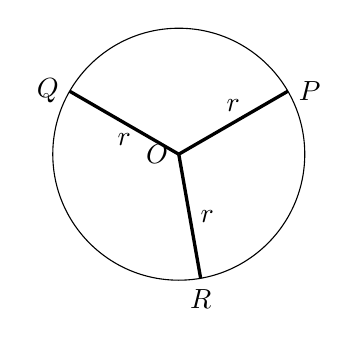
\begin{tikzpicture}[>=latex, scale=.8]
    \draw (0,0) circle (2);
\draw[very thick](0,0)node[left]{$O$}--node[above]{$r$}(30:2)node[right]{$P$};
\draw[very thick](0,0)--node[below]{$r$}(150:2)node[left]{$Q$};
\draw[very thick](0,0)--node[right]{$r$}(-80:2)node[below]{$R$};
    \end{tikzpicture}
    \caption{}
    \end{minipage}
    \begin{minipage}[t]{0.48\textwidth}
    \centering
    \begin{tikzpicture}[>=latex, scale=.8]
        \draw  (0,0) circle (2);
\draw[very thick] (60:2)--node[below]{弦}(135:2);
\draw[very thick] (-10:2)--node[below]{直径}(170:2);
\draw (-135:2) [fill=black]circle(1.5pt)node[left]{$E$};
\draw (-45:2) [fill=black]circle(1.5pt)node[right]{$F$};
\draw[very thick]  (-135:2) arc (-135:-45:2);
\node at (0,-2) [below=2pt]{弧};


    \end{tikzpicture}
    \caption{}
    \end{minipage}
    \end{figure}

从圆的定义,不难直接推知:
\begin{itemize}
    \item 两个圆能够重合的充要条件是两个圆的半径相等.
    \item 半径相等的圆叫做\textbf{等圆},\textbf{等圆的半径相等直径相等}.
\end{itemize}

从圆的定义,我们还可以看出,一个圆把它所在的平面
分为三部分(图4.3):
\begin{enumerate}
    \item 圆本身,即与圆心的距离等于半径的点所构成的集
合.其中任何一点都叫做圆上的点.
\item 圆的内部,与圆心的距离小于半径的点所构成的集
合.圆的内部又简称\textbf{圆内};其中任何一点都叫做圆内的点.
\item 圆的外部:与圆心的距离大于半径的点所构成的集
合;圆的外部又简称\textbf{圆外},其中任何一点都叫做圆外的点.
\end{enumerate}

\begin{figure}[htp]\centering
    \begin{minipage}[t]{0.48\textwidth}
    \centering
\begin{tikzpicture}[>=latex, scale=.8]
    \draw[pattern=north west lines] (0,0) circle (2);
    \draw[thick] (0,0)--node[left=3.5pt, fill=white]{$r$}(60:2);
    \end{tikzpicture}
    \caption{}
    \end{minipage}
    \begin{minipage}[t]{0.48\textwidth}
    \centering
    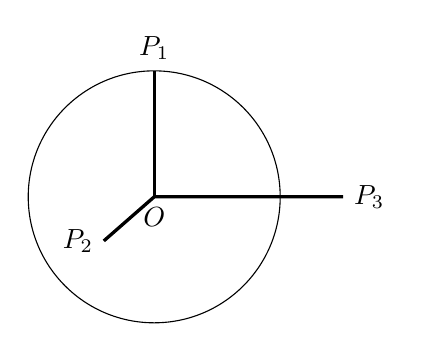
\begin{tikzpicture}[>=latex, scale=.8]
        \draw  (0,0) circle (2);
\draw[very thick](-.8,-.7)node[left]{$P_2$}--(0,0)node[below]{$O$}--(3,0)node[right]{$P_3$};
\draw[very thick](0,0)--(0,2)node[above]{$P_1$};

    \end{tikzpicture}
    \caption{}
    \end{minipage}
    \end{figure}

通常我们说的圆面,指的是由圆所围成的平面部分,也
就是与圆心的距离小于或等于半径的点所构成的集合.如图
4.3中阴影部分.

由上述定义可知,$\odot(O,r)$与平面上任一点P的位置关
系,有下述的性质(图4.4).
\begin{enumerate}
    \item 点$P$在$\odot(O,r)$上的充要条件是$\overline{OP}=r$;
    \item 点$P$在$\odot(O,r)$内的充要条件是$\overline{OP}<r$;
    \item 点$P$在$\odot(O,r)$外的充要条件是$\overline{OP}>r$.
\end{enumerate}

\begin{ex}
\begin{enumerate}
    \item 根据下述条件画圆
\begin{enumerate}
\item 已知定点$O$, 以$O$为圆心画一圆使半径等于2厘
米.
\item 已知两个定点$O$、$P$, 画$\odot(O,\overline{OP})$.
\item 先画一条$\overline{AB}$, 再画出以$\overline{AB}$
为直径的圆.
\end{enumerate}

\item 把以下命题写成“若一则”形式
\begin{enumerate}
\item 点$P$在$\odot(O,r)$上的充分条件是
$\overline{OP}=r$;
\item 点$P$在$\odot(O,r)$内的必要条件是
$\overline{OP}<r$;
\item 点$P$在$\odot(O,r)$外的充分条件是
$\overline{OP}>r$.
\end{enumerate}


\item 以点$O$为圆心,$r_1$、$r_2$为半径画两个圆.说出满足下列条
件的点$X$在平面上的位置范围.
\begin{multicols}{2}
\begin{enumerate}
    \item $\overline{OX} >r_2$
    \item $\overline{OX} \le r_1$
    \item $r_1<\overline{OX}<r_2 $
    \item $\overline{OX}=r_1 $
    \item $\overline{OX}<r_1 $
\end{enumerate}
\end{multicols}

\item 已知一个$\odot O$的直径长是4cm. 说出满足下列条件的$P$点
的可能位置:
\begin{multicols}{2}
    \begin{enumerate}
        \item $\overline{OP} >2$cm
        \item $\overline{OP} \ge 2$cm
        \item $\overline{OP} <2$cm
        \item $\overline{OP} =0$
    \end{enumerate}
    \end{multicols}

\item 求证一个圆的直径
是这个圆中最长的弦.

(提示:按图中所示证$\overline{AB}>\overline{CD}$).
\begin{center}
    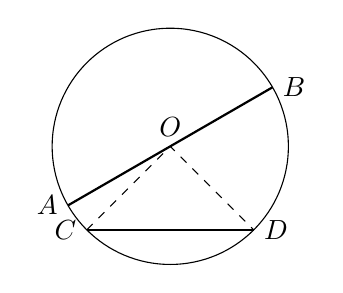
\begin{tikzpicture}
        \draw (0,0) circle (1.5);
\draw[thick] (-150:1.5)node[left]{$A$}--node[above]{$O$}(30:1.5)node[right]{$B$};
\draw[thick]  (-135:1.5)node[left]{$C$}--(-45:1.5)node[right]{$D$};
\draw[dashed](-135:1.5)--(0,0)--(-45:1.5);
    \end{tikzpicture}
\end{center}
\end{enumerate}
\end{ex}

\subsection{不共线的三点确定一圆}
我们已知,如果知道了圆心的位置和半径长,那么圆的
位置和大小也就确定了.现在我们来研究经过一个点;经过
两个点;经过三个点可分别作出几个圆?
    
已知一个点$A$, 很明显,以$A$点以外的任何点为圆心,
以这点到$A$点的距离为半径所作的圆都经过$A$点(图4.5).
因此,\textbf{经过一点可以作无数个圆}.
\begin{figure}[htp]\centering
	\begin{minipage}[t]{0.48\textwidth}
		\centering
		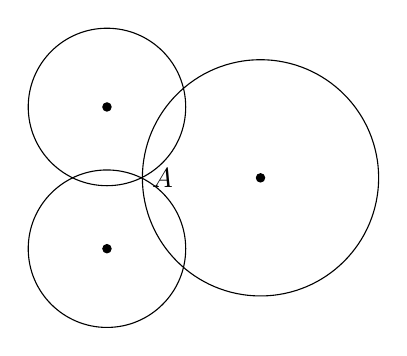
\begin{tikzpicture}[>=latex, scale=1]
\draw (0,.9) circle (1);
\draw (0,-.9) circle (1);
\draw (1.95,0) circle (1.5);
\foreach \x/\y in{0/.9, 0/-.9, 1.95/0}
{
    \draw (\x,\y)[fill=black]circle(1.5pt);
}
\node at (1.95-1.5,0)[right]{$A$};

		\end{tikzpicture}
		\caption{}
	\end{minipage}
	\begin{minipage}[t]{0.48\textwidth}
		\centering
		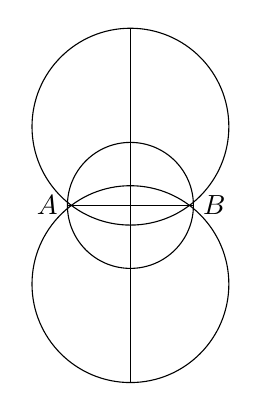
\begin{tikzpicture}[>=latex, scale=1]
	\draw (0,1) circle (1.25);
	\draw (0,-1) circle (1.25);
	\draw (0,0) circle (.8);	
	\draw (-.8,0)node[left]{$A$}--(.8,0)node[right]{$B$}   ;	
	\draw(0,2.25)--(0,-2.25);
		\end{tikzpicture}
		\caption{}
	\end{minipage}
\end{figure}

经过两个已知点$A$、$B$,可以作多少个圆呢(图4.6)?
由于经过$A$、$B$两点的圆的圆心到$A$点与$B$点的距离应相等,而
和$A$、$B$两点距离相等的点仅在$AB$的垂直平分线上,所以,
以$AB$的垂直平分线上任一点为圆心,以这点到$A$点(或$B$
点)的距离为半径所作的圆都经过$A$、$B$两点.因此,\textbf{经过
两点也可以作无数个圆,且圆心都在连结这两点的线段的垂
直平分线上}.

现在我们来研究,经过$A$、$B$、$C$三点可以作多少个圆的
问题?

\begin{figure}[htp]\centering
	\begin{minipage}[t]{0.48\textwidth}
		\centering
		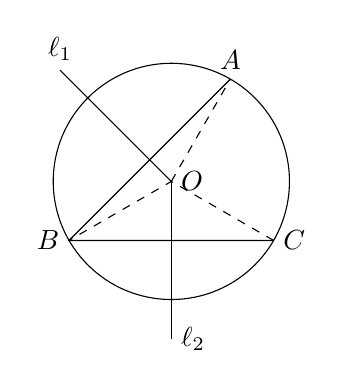
\begin{tikzpicture}[>=latex, scale=1]
\draw (0,0)node[right]{$O$} circle (1.5);
\draw[dashed] (-30:1.5)node[right]{$C$}--(0,0)--(-150:1.5)node[left]{$B$};
\draw (-30:1.5)--(-150:1.5)--(60:1.5);
\draw[dashed] (0,0)--(60:1.5)node[above]{$A$};
\draw (0,0)--(-90:2)node[right]{$\ell_2$};
\draw (0,0)--(135:2)node[above]{$\ell_1$};
		\end{tikzpicture}
		\caption{}
	\end{minipage}
	\begin{minipage}[t]{0.48\textwidth}
		\centering
		\begin{tikzpicture}[>=latex, scale=1]
\draw (0,0)--(5,0);
\foreach \x/\xtext in{1/A,2.5/B,4.5/C}
{
    \draw (\x,0)node[below]{$\xtext$}[fill=black] circle(1.5pt) ;
}
\draw[thick] (1.5,-1.5)--(1.5,1.5)node[above]{$\ell_1$};
\draw[thick] (4,-1.5)--(4,1.5)node[above]{$\ell_2$};
		\end{tikzpicture}
		\caption{}
	\end{minipage}
\end{figure}

我们知道,经过$A$、$B$两点的圆的圆心必定在$\overline{AB}$的垂
直平分线上(图4.7中的$\ell_1$),经过$B$、$C$两点的圆的圆心
又必定在$\overline{BC}$的垂直平分线上(图4.7中的$\ell_2$),因而经过
$A$、$B$、$C$三点的圆的圆心必定是直线$\ell_1$和$\ell_2$的交点$O$, 由
于$\overline{OA}=\overline{OB}=\overline{OC}$, 所以以$O$为圆心$\overline{OA}$为半径的圆经过
$A$、$B$、$C$三点.

这样一来,能不能说经过三个点就可作一个圆呢?我们
再来看图4.8中所示的三点$A$、$B$、$C$,它们是在同一条直线
上的,这时$\overline{AB}$和$\overline{BC}$的垂直平分线$\ell_1$和$\ell_2$都垂直于同一条直
线,于是$\ell_1\parallel \ell_2$, $\ell_1$和$\ell_2$便没有交点,这就说明了经过$A$、
$B$、$C$三点的圆的圆心根本不存在,所以也就没有圆都经过
$A$、$B$、$C$三点.因此,我们不能笼统地说经过三个点可作一
个圆.如果$A$、$B$、$C$三点在同一条直线上(叫做共线的点),
便没有圆经过这三点;如果$A$、$B$、$C$三点不在同一条直线
上(叫做不共线的点),那么$\overline{AB}$与
$\overline{BC}$的垂直平分线必相交
(为什么?),这时,就可作一个圆经过这三点,又由于
$\overline{AB}$和$\overline{BC}$的垂直平分线都只有一条,所以它们的交点也是唯
一的,从而$\overline{OA}$的长也是唯一的,所以经过$A$、$B$、$C$三点也
只能作一个圆.

于是,我们便得到确切的结论:

\begin{blk}{定理}
过不共线的三个点,可以作一个圆且只可以作一
个圆.    
\end{blk}
 
由上述讨论,我们还可看到一个圆的圆心到圆的任一条
弦的两个端点的距离相等,因而可得:

\begin{blk}{推论1}
圆的任一条弦的垂直平分线都通过圆心.
\end{blk}
 
由于任一个$\triangle ABC$的三个顶点不共线,因此经过$A$、$B$、
$C$三个顶点可以作一个圆,且只可以作一个圆$\odot O$(图4.9),这个圆叫做$\triangle ABC$的\textbf{外接圆},它的圆心$O$叫做$\triangle ABC$的\textbf{外心},而$\triangle ABC$叫做$O$的\textbf{内接三角形}.由于$\overline{OA}=\overline{OB}=\overline{OC}$, 
$O$点一定在三边的垂直平分线上,于是又可得:

\begin{figure}[htp]
    \centering
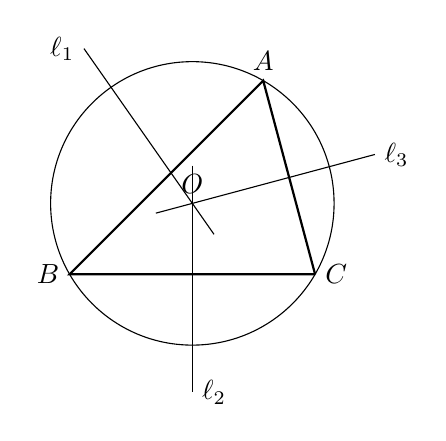
\begin{tikzpicture}[>=latex, scale=1.2]
\draw (0,0)node[above]{$O$} circle (1.5);
\draw[thick] (-30:1.5)node[right]{$C$}--(-150:1.5)node[left]{$B$}--(60:1.5)node[above]{$A$}--(-30:1.5);
\draw(0,.4)--(0,-2)node[right]{$\ell_2$};
\draw(15+180:.4)--(15:2)node[right]{$\ell_3$};
\draw(125-180:.4)--(125:2)node[left]{$\ell_1$};

    \end{tikzpicture}
    \caption{}
\end{figure}

\begin{blk}{推论2}
    三角形的三边的垂直平分线相交于一点,这个
点就是三角形的外心.
\end{blk}
 
由推论2我们又可得到:
 
\begin{blk}{推论3}
   三角形的三条高线相交于一点.
\end{blk}

已知:$AD$、$BE$、$CF$是$\triangle ABC$的三条高线(图4.10).
求证:$AD$、$BE$、$CF$相交于一点.

\begin{figure}[htp]
    \centering
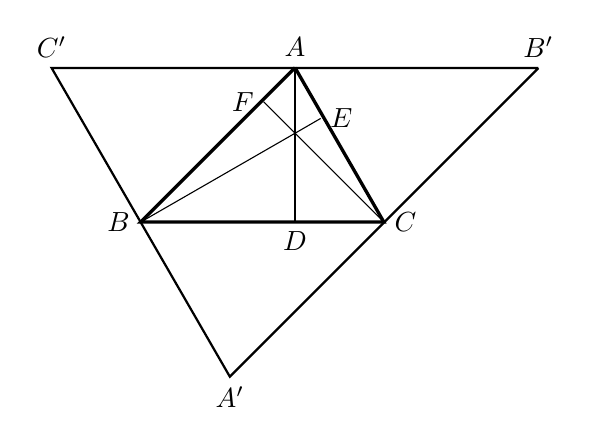
\begin{tikzpicture}[scale=.8]
\draw[thick] (15:4)node[above]{$B'$}--(180-15:4)node[above]{$C'$}--(-90-15:4)node[below]{$A'$}--(15:4);
\draw[very thick] (0,1.04)node[above]{$A$}--(-2.45,-1.41)node[left]{$B$}--(1.41,-1.41)node[right]{$C$}--(0,1.04);
\draw (0,1.04)--(0,-1.41)node[below]{$D$};
\draw (-2.45,-1.41)--(0,0)--(0.406,.235)node[right]{$E$};
\draw (1.41,-1.41)--(0,0)--(-.5,.5)node[left]{$F$};
\end{tikzpicture}
    \caption{}
\end{figure}

\begin{proof}
    经过$\triangle ABC$的各顶点$A$、$B$、$C$分别作对边的平
行线,设它们分别相交于$B'$、$C'$、$A'$各点,于是$AD\bot B'C'$,
$BE\bot C'A'$, $CF\bot A'B'$(为什么?),又因为四边形$BCAC'$和
$BCB'A$都是平行四边形(为什么?).

$\therefore\quad \overline{CA}=\overline{BC}=\overline{AB'}$, 于是$A$是$\overline{B'C'}$的中点.

同理,$B$是$\overline{A'C'}$的中点,$C$是$\overline{A'B'}$的中点,因此,$AD$、
$BE$、$CF$分别是$\triangle A'B'C'$的三边上的垂直平分线,由推论2
可知$AD$、$BE$和$CF$相交于一点.
\end{proof}


图4.10中,画出的是锐角三角形,如$\triangle ABC$是钝角三
角形,上述证明过程同样适用,同学可自己验证.

三角形的三条高线的交点叫做\textbf{三角形的垂心}.

\begin{example}
    求作一条已知弧的圆心.
\end{example}

已知$\wideparen{EF}$(图4.11).

求作:$\wideparen{EF}$所在圆的圆心.

作法
\begin{enumerate}
    \item 在$\wideparen{EF}$
    上任取三点$A$、$B$、$C$, 并且作$\overline{AB}$、$\overline{BC}$.
    \item 分别作$\overline{AB}$、$\overline{BC}$的垂直平分线$\ell_1$和$\ell_2$, 设它们
    的交点为$O$, $O$点就是所求作的圆心.
\end{enumerate}

\begin{proof}
    $\because\quad A$、$B$、$C$三点在$\wideparen{EF}$上(作法)

$\therefore\quad \wideparen{EF}$是经过$A$、$B$、$C$的圆的一部分.

又$\because\quad O$是经过$A$、$B$、$C$的圆的圆心,

$\therefore\quad O$是$\wideparen{EF}$所在圆的圆心.
\end{proof}

\begin{figure}[htp]\centering
    \begin{minipage}[t]{0.48\textwidth}
    \centering
  \begin{tikzpicture}[>=latex, scale=1]
\tkzDefPoint(150:2.5){A}
\tkzDefPoint(110:2.5){B}
\tkzDefPoint(40:2.5){C}
\tkzDefPoint(160:2.5){E}
\tkzDefPoint(20:2.5){F}
\tkzDrawSegments[very thick](A,B B,C)
\tkzDefPoints{0/0/O}
\tkzDefPointBy[projection = onto A--B](O)\tkzGetPoint{O'}
\tkzDefPointBy[projection = onto C--B](O)\tkzGetPoint{O''}
\tkzDrawLines[add=.3 and .7](O,O' O,O'')
\tkzAutoLabelPoints[center=O](A,B,C,E,F)
\tkzDrawArc[color=black, thick](O,F)(E)
\tkzLabelPoints[right](O)
\node at (-2,3){$\ell_1$};
\node at (1,3){$\ell_2$};
    \end{tikzpicture}
    \caption{}
    \end{minipage}
    \begin{minipage}[t]{0.48\textwidth}
    \centering
    \begin{tikzpicture}[>=latex, scale=1]
\tkzDefPoints{0/0/B, 4/0/C, 3/3/A}
\tkzDrawPolygon(A,B,C)
\tkzDefTriangleCenter[circum](A,B,C)  \tkzGetPoint{O}
\tkzDefTriangleCenter[ortho](A,B,C)  \tkzGetPoint{H}
\tkzDefPointBy[projection= onto B--C](O) \tkzGetPoint{L}
\tkzDefPointBy[projection= onto B--A](O) \tkzGetPoint{M}
\tkzInterLL(A,C)(B,H)\tkzGetPoint{B'}
\tkzInterLL(B,C)(A,H)\tkzGetPoint{D}
\tkzInterLL(A,B)(C,H)\tkzGetPoint{C'}
\tkzDefMidPoint(B,H) \tkzGetPoint{K}
\tkzDrawSegments(A,D C,C' B,B' O,M O,L M,K L,K)
\tkzLabelPoints[below](B,C,L,D)
\tkzLabelPoints[above](A,M)
\tkzLabelPoints[right](O)
\tkzLabelPoints[above right](H)
\tkzLabelPoints[above left](K)
\tkzDrawPoints(O,H,K)
    \end{tikzpicture}
    \caption{}
    \end{minipage}
    \end{figure}

\begin{example}
    已知$O$和$H$各是$\triangle ABC$的外心和垂心,$OL\bot \overline{BC}$
    于$L$(图4.12). 
    求证:$\overline{OL}=\frac{1}{2}\overline{AH}$
\end{example}

\begin{proof}
    已知$OL\bot \overline{BC}$于$L$点,作$OM\bot \overline{AB}$于$M$点,由
    于$O$是$\triangle ABC$的外心,所以$L$、$M$分别是$\overline{BC}$、$\overline{AB}$的中点.
    取$\overline{BH}$的中点$K$, 作$\overline{MK}$, $\overline{LK}$, 
 
$\because\quad     MK\parallel AH,\quad OL\parallel AH$,

$\therefore\quad MK\parallel OL$,

同理可证,$LK\parallel OM$,

$\therefore\quad OMKL$是平行四边形,

$\therefore\quad \overline{OL}=\overline{MK}=\frac{1}{2}\overline{AH}$
\end{proof}

\begin{ex}
\begin{enumerate}
    \item 分别作一个锐角三角形、一个直角三角形和一个钝角三
    角形的外接圆,并说出它们的外心的位置各有什么特点.
    \item 经过任意四点,可不可以作一个圆?试举例说明.
    \item 分别作出一个锐角三角形、一个直角三角形和一个钝角
    角形的套心,并说出它们的位置各有什么特点.
    \item 已知$H$是$\triangle ABC$的垂心,
    $D$、$E$、$F$是三高的垂足.试分别说出$\triangle HBC$、$\triangle HAC$、$\triangle HAB$的垂心各是图中哪一点.
\end{enumerate}
\end{ex}

\begin{figure}[htp]
    \centering
\begin{tikzpicture}
    \tkzDefPoints{0/0/B, 4/0/C, 1.8/2.5/A}
\tkzDrawPolygon(A,B,C)
\tkzDefTriangleCenter[ortho](A,B,C)  \tkzGetPoint{H}
\tkzInterLL(A,C)(B,H)\tkzGetPoint{E}
\tkzInterLL(B,C)(A,H)\tkzGetPoint{D}
\tkzInterLL(A,B)(C,H)\tkzGetPoint{F}
\tkzDrawSegments(A,D B,E C,F)
\tkzLabelPoints[below](B,C,D)
\tkzLabelPoints[left](F)
\tkzLabelPoints[right](E)
\tkzLabelPoints[above](A)
\tkzLabelPoints[below right](H)
\end{tikzpicture}
    \caption*{第4题}
\end{figure}

\subsection{圆的对称性}
已知$\odot O$(图4.13), 在$O$上任取一点$A$, 引直径$\overline{AA'}$, 
则$\overline{AA'}$被圆心$O$平分.这就是说$A'$是以点$O$为对称中心的
点$A$的对称点,如果在$\odot O$上再取$B,C,D,\ldots$, 并引直径
$\overline{BB'},\overline{CC'},\overline{DD'},\ldots$, 那么点$B',C',D',\ldots$ 也都分别是
以$O$为对称中心的点$B,C,D,\ldots$的对称点.这就说明
了$\odot O$上以$O$为对称中心的任何点的对称点都在$\odot O$上.由
此可知:\textbf{圆是中心对称形;圆心是它的对称中心}.

已知$\overline{AA'}$是$\odot O$的任一条直径(图4.14),作直径$\overline{BB'}\bot 
\overline{AA'}$, 把$\odot O$左边部分沿着直线$AA'$翻折过来,由于$\overline{BB'}\bot \overline{AA'}$, $\overline{OB'}=\overline{OB}$, 那么$B$点就与$B'$点重合,因为经过$A$、
$B'$、$A'$三点只可以作一个圆,所以以$A$、$A'$为端点,经过
$B'$点的弧只有一条,因此$\wideparen{ABA'}$与
$\wideparen{AB'A'}$重合.由此可知,
圆是轴对称图形,任一条通过圆心的直线都是它的对称轴.

\begin{figure}[htp]\centering
    \begin{minipage}[t]{0.48\textwidth}
    \centering
  \begin{tikzpicture}[>=latex, scale=1]
\tkzDefPoint(20:1.5){A'}
\tkzDefPoint(-30:1.5){B'}
\tkzDefPoint(200:1.5){A}
\tkzDefPoint(150:1.5){B}
\tkzDefPoint(90:1.5){C}
\tkzDefPoint(-90:1.5){C'}
\tkzDefPoint(0,0){O}
\tkzDrawCircle[very thick](O,A)
\tkzDrawSegments[thick](A,A' B,B' C,C')
\tkzAutoLabelPoints[center=O](A,A',B,B',C,C')
\tkzLabelPoints[above right](O)
    \end{tikzpicture}
    \caption{}
    \end{minipage}
    \begin{minipage}[t]{0.48\textwidth}
    \centering
    \begin{tikzpicture}[>=latex, scale=1]
      \tkzDefPoint(0:1.5){B'}
\tkzDefPoint(180:1.5){B}
\tkzDefPoint(90:1.5){A}
\tkzDefPoint(-90:1.5){A'}
\tkzDefPoint(0,0){O}
\tkzDrawCircle[very thick](O,A)
\tkzDrawSegments[thick](A,A' B,B')
\tkzAutoLabelPoints[center=O](B,B')
\draw[dashed](A)node[above right]{$A$}--(0,2.5);
\draw[dashed](A')node[below right]{$A'$}--(0,-2.5);
    \end{tikzpicture}
    \caption{}
    \end{minipage}
    \end{figure}

由上述圆的对称性,我们可推出许多圆的重要性质.

\begin{blk}
    {推论1} 圆被它的任何一条直径截出的两段弧相等.这两
段弧都叫做半圆.
\end{blk}

小于半圆的弧叫做\textbf{劣弧},大于半圆的弧叫做\textbf{优弧}.以后
说到弧,如不特别指明,一般都指的是劣弧.

\begin{blk}
    {推论2} 一圆的直径垂直于一条非直径的弦的充分必要
条件是这直径平分这条弦或平分这条弦所对的弧.
\end{blk}

我们来证必要性,充分性留给同学们自证.

已知:$\odot O$中,直径$\overline{CD}\bot $弦$\overline{AB}$于$E$点(图4.15).

求证:$\overline{AE}=\overline{BE}$, $\wideparen{AD}=\wideparen{BD}$, $\wideparen{AC}=\wideparen{BC}$.

\begin{proof}
$\because\quad \overline{CD}$是$\odot O$的直径

$\therefore\quad $直线$CD$是$\odot O$的对称轴.

又$\because\quad CD\bot AB$于$E$点

$\therefore\quad CD$也是等腰$\triangle OAB$的
对称轴.以$CD$为轴把图形翻
折叠合时,半圆$\wideparen{CAD}$与半圆$\wideparen{CBD}$重合,$\overline{AE}$与
$\overline{BE}$
重合.$A$点与$B$点重合,
$\wideparen{AD}$与$\wideparen{BD}$, $\wideparen{AC}$与
$\wideparen{BC}$都重合

$\therefore\quad \overline{AE}=\overline{BE},\quad 
\wideparen{AD}=\wideparen{BD},\quad 
\wideparen{AC}=\wideparen{BC}$.
\end{proof}

\begin{figure}[htp]\centering
    \begin{minipage}[t]{0.48\textwidth}
    \centering
  \begin{tikzpicture}[>=latex, scale=1]
\tkzDefPoints{0/0/O, 0/2/C, 0/-2/D}
\tkzDefPoint(-30:2){B}
\tkzDefPoint(-150:2){A}
\tkzAutoLabelPoints[center=O](A,B,C,D)
\tkzLabelPoints[above left](O)
\tkzInterLL(O,D)(A,B)\tkzGetPoint{E}
\tkzLabelPoints[above right](E)
\tkzDrawSegments(A,B C,D A,O B,O)
\tkzDrawCircle[thick](O,C)
    \end{tikzpicture}
    \caption{}
    \end{minipage}
    \begin{minipage}[t]{0.48\textwidth}
    \centering
    \begin{tikzpicture}[>=latex, scale=1]
\tkzDefPoints{0/0/O, 0/3.5/C, 0/-1/D, 0/2/E}
\tkzDefPoint(30:2){B}
\tkzDefPoint(150:2){A}
\tkzDrawLines[add=.1 and .1](C,D)
\tkzLabelPoints[right](C,D)
\tkzLabelPoints[below](A,B)
\tkzLabelPoints[below right](E)
\tkzDrawArc[thick, color=black](O,B)(A)
\tkzDrawSegments[thick](A,B)
\tkzCompasss(A,C B,C A,D B,D)


    \end{tikzpicture}
    \caption{}
    \end{minipage}
    \end{figure}



\begin{example}
    平分一条已知弧.

已知:$\wideparen{AB}$(图4.16).

求作:平分$\wideparen{AB}$的点.

作法
\begin{enumerate}
    \item 作$\overline{AB}$
    \item 作$\overline{AB}$的垂直平分线$CD$交$\wideparen{AB}$于$E$点.则$E$点就
是所求作的点.
\end{enumerate}
\end{example}

\begin{proof}
$\because\quad CD$是$\overline{AB}$的垂直平分线(作法).

$\therefore\quad CD$ 必通过圆心,

$\therefore\quad \wideparen{AE}=\wideparen{BE}$ (推论2).

$\therefore\quad E$点平分$\wideparen{AB}$.
\end{proof}

\begin{example}
    已知大小两圆有公共圆心$O$, 大圆的弦交小圆于
$C$、$D$ (图4.17).

求证:$\overline{AC}=\overline{BD}$.
\end{example}

\begin{proof}
    作$\overline{OM}\bot \overline{AB}$于$M$点,则$\overline{AM}=\overline{BM}$, $\overline{CM}=\overline{DM}$.

$\therefore\quad     \overline{AM}-\overline{CM}=\overline{BM}-\overline{DM}$.
    
$\therefore\quad \overline{AC}=\overline{BD}$
\end{proof}

\begin{figure}[htp]\centering
    \begin{minipage}[t]{0.48\textwidth}
    \centering
  \begin{tikzpicture}[>=latex, scale=1]
\tkzDefPoints{0/0/O, 0/-1/M, -1.5/-1/A, 1.5/-1/B, -1/-1/C, 1/-1/D}
\tkzDrawCircle[thick](O,C)
\tkzDrawCircle[thick](O,A)
\tkzDrawSegments[thick](A,B O,M)
\tkzLabelPoints[below](A,B,C,D,M)
\tkzLabelPoints[above](O)

    \end{tikzpicture}
    \caption{}
    \end{minipage}
    \begin{minipage}[t]{0.48\textwidth}
    \centering
    \begin{tikzpicture}[>=latex, scale=1]
\tkzDefPoints{0/0/O}
\tkzDefPoint(45:1.8){B}
\tkzDefPoint(135:1.8){A}
\tkzDefPoint(-30:1.8){D}
\tkzDefPoint(-150:1.8){C}
\tkzDefMidPoint(A,B)\tkzGetPoint{E}
\tkzDefMidPoint(C,D)\tkzGetPoint{F}
\tkzAutoLabelPoints[center=O](A,B,C,D)
\tkzLabelPoints[above](E)
\tkzLabelPoints[below](F)
\tkzDrawSegments(A,O C,O A,B C,D E,F)
\tkzLabelPoints[right](O)
\tkzDrawCircle[thick](O,A)
    \end{tikzpicture}
    \caption{}
    \end{minipage}
    \end{figure}

    
\begin{example}
    已知$\odot O$的两条平行弦$\overline{AB}=6$cm, $\overline{CD}=8$cm
    且
    $AB$和$CD$间的距离是7cm, 求$\odot O$的半径长(图4.18).
\end{example}

\begin{solution}
    作$OE\bot \overline{AB}$
于$E$点,延长$\overline{EO}$交$\overline{CD}$于$F$点.

$\because\quad AB\parallel CD$,

$\therefore\quad OF\bot CD$,

$\therefore\quad \overline{EF}$为$\overline{AB}$和$\overline{CD}$的公垂线段,且$\overline{EF}=7$cm,
$\overline{AE}=\frac{1}{2}\overline{AB}=3$cm, $\overline{CF}=
\frac{1}{2}\overline{CD}=4$cm.

设$\overline{OA}=\overline{OC}=x$, $\overline{OE}=y$, 则由勾股定理可得方程组:
\[\begin{cases}
    x^2=3^2+y^2\\
    x^2=(7-y)^2+4^2
\end{cases}\]
解这个方程组,舍去不合理的根得:
\[\begin{cases}
    x=5\\y=4
\end{cases}\]

答:$\odot O$的半径是5cm.
\end{solution}

\begin{ex}
\begin{enumerate}
    \item 把本节推论2用“若一则”
    形式写出互逆的定理.
    \item 作出图中圆的圆心.
    \item 已知$\odot(0,5{\rm cm})$, 它的一条弦$\overline{AB}=8$cm, 点$M$是
    $\overline{AB}$的
    中点,求$\overline{OM}$的长.
    \item 已知一圆的半径是25cm, 一弧所对的弦长是48cm, 求这
    弧的一半所对的弦长.
    \item 求证圆中的非直径的两弦必不能互相平分
    (提示:用反证法).
\end{enumerate}
\end{ex}

\begin{figure}[htp]
    \centering
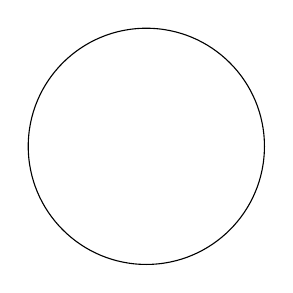
\begin{tikzpicture}
    \draw(0,0) circle (1.5);
\end{tikzpicture}
    \caption*{第2题}
\end{figure}

\subsection{弧、弦和弦心距之间的关系}
圆的圆心到一条弦的距离,叫做这条弦的弦心距,例如
在图4.19中,$\overline{AB}$是$\odot O$的一条弦,$\overline{OE}\bot \overline{AB}$于$E$点,$\overline{OE}$
的长就是弦
$\overline{AB}$的弦心距.下面我们来学习弧、弦和弦心距
之间的关系.

\begin{blk}
    {定理} 在同圆或等圆中,两条弧相等的充要条件是它们
所对的弦相等,或它们所对的弦的弦心距相等.
\end{blk}

\begin{figure}[htp]
    \centering
    \begin{tikzpicture}[>=latex]
 \tkzDefPoints{0/0/O}
\tkzDefPoint(-60:2){B}
\tkzDefPoint(-120:2){A}
\tkzDefPoint(0:2){C}
\tkzDefPoint(60:2){D}
\tkzDefMidPoint(A,B)\tkzGetPoint{E}
\tkzDefMidPoint(C,D)\tkzGetPoint{F}
\tkzDrawSegments[very thick](A,B C,D)
\tkzDrawSegments(O,A O,B O,C O,D O,E O,F)
\tkzLabelPoints[above left](O)
\tkzAutoLabelPoints[center=O](A,B,C,D)
\tkzLabelPoints[above right](E)
\tkzLabelPoints[left](F)
\tkzDrawCircle[thick](O,A)       

\draw[->](-50:1.2) arc (-50:-10:1.2);
    \end{tikzpicture}
    \caption{}
\end{figure}

我们来证条件的必要性,充分性由同学们自证:

已知:在$\odot O$中,$\wideparen{AB}=\wideparen{CD}$, 
$OE\bot  AB$于$E$点,$OF\bot CD$于
$F$点(图4.19).

求证:$\overline{AB}=\overline{CD}$, $\overline{OE}=\overline{OF}$.

\begin{proof}
    作半径$\overline{OA}$、$\overline{OB}$、$\overline{OC}$、$\overline{OD}$. 把$\wideparen{AB}$连同经过
两端的半径绕着$O$点,依箭头所指的方向旋转,使半径$\overline{OA}$
和半径$\overline{OC}$重合.

$\because\quad \wideparen{AB}=\wideparen{CD}$.

$\therefore\quad \wideparen{AB}$与$\wideparen{CD}$重合,弦$\overline{AB}$与弦$\overline{CD}$重合.

又$\because\quad $从一点到一条直线只可以作一条垂线,

$\therefore\quad \overline{OE}$与$\overline{OF}$
也重合

$\therefore\quad \overline{AB}=\overline{CD},\quad \overline{OE}=\overline{OF}$.
\end{proof}

对于等圆情况的证明,只要使两圆重合就可以了.

这个定理告诉我们,在同圆或等圆中,“弧相等”、
“弦相等”、“弦心距相等”它们当中只要有一个是对的,
其它两个也一定是对的.这就是说:

\begin{blk}{}
   “弧相等”$\Longleftrightarrow$“弦相等”$\Longleftrightarrow$“弦心距相等” 
\end{blk}

\begin{example}
    已知(图4.20),$\overline{OE}$是$\odot O$中的半径,$F$是$\overline{OE}$上任一
点,$\overline{AB}$和$\overline{CD}$为过$F$点的弦且$\angle AFO=\angle DFO$.

求证:$\overline{AB}=\overline{CD}$
\end{example}

\begin{figure}[htp]
    \centering
\begin{tikzpicture}
\tkzDefPoints{0/0/O, 2/0/E}
\tkzDefPoint(70:2){A}
\tkzDefPoint(-70:2){D}
\tkzDefPoint(-20:2){B}
\tkzDefPoint(20:2){C}
\tkzDefMidPoint(A,B)\tkzGetPoint{M}
\tkzDefMidPoint(C,D)\tkzGetPoint{N}
\tkzInterLL(O,E)(A,B)\tkzGetPoint{F}
\tkzLabelPoints[left](O)
\tkzAutoLabelPoints[center=O](A,B,C,D,E)
\tkzDrawSegments[thick](O,M O,N A,B C,D O,E)
\tkzDrawCircle[very thick](O,A)
\tkzLabelPoints[above](F)
\tkzLabelPoints[above](M)
\tkzLabelPoints[below](N)


\end{tikzpicture}
    \caption{}
\end{figure}


\begin{proof}
作$\overline{OM}\bot \overline{AB}$于$M$点,$\overline{ON}\bot \overline{CD}$ 于$N$点,在直角
$\triangle OMF$与直角$\triangle ONF$中,

$\because\quad \angle MFO=\angle NFO,\quad \overline{OF}=\overline{OF}$.

$\therefore\quad \triangle OMF\cong \triangle ONF$

$\therefore\quad \overline{OM}=\overline{ON}$.

$\therefore\quad \overline{AB}=\overline{CD}$.
\end{proof}

\begin{ex}
\begin{enumerate}
    \item 把本节定理用“若—则”形式写出互逆的定理.
    \item 以$\angle A$的平分线上任一点$O$为圆心,大于$O$点到边的距
    离之长为半径作一个圆,那么这圆在$A$的两边上截出
    的两条弦相等.
    \item 在$\odot O$中,已知$\overline{AB}$是一条直径,$\overline{AC}$和$\overline{AD}$是分属于
    $\overline{AB}$两侧的两条相等的弦,
    求证:$AB$平分$\angle CAD$
    \item 如图,$\odot O$内相等的两弦
    $\overline{AB}$、$\overline{CD}$相交于$E$点,
    求证
    \begin{enumerate}
        \item $\wideparen{AC}=\wideparen{BD}$
        \item $\overline{AE}=\overline{DE}$
        \item $\overline{BE}=\overline{CE}$
    \end{enumerate}
\end{enumerate}
\end{ex}

\begin{figure}[htp]
    \centering
\begin{tikzpicture}[scale=.8]
\tkzDefPoints{0/0/O}
\tkzDefPoint(30:2){A}
\tkzDefPoint(-140:2){D}
\tkzDefPoint(-90:2){B}
\tkzDefPoint(-20:2){C}
\tkzInterLL(C,D)(A,B)\tkzGetPoint{E}
\tkzAutoLabelPoints[center=O](A,B,C,D)
\tkzLabelPoints[above left](E)
\tkzDrawSegments[thick](A,B C,D)
\tkzDrawCircle[very thick](O,A)
\end{tikzpicture}
    \caption*{第4题}
\end{figure}

\subsection{两圆的位置关系}
不重合的两圆,它们的位置关系,有以下五种情况:
\begin{enumerate}
\item 一圆在另一圆的外部,这种位置关系叫做\textbf{两圆相
离},如图4.21(1).这时,两圆没有公共点.
\item 两圆只有一个公共点且其中一圆上的其它各点都
在另一圆的外部,这种位置关系叫做\textbf{两圆外切},如图
4.21(2). 这个公共点叫做两圆的\textbf{切点}.
\item 两圆有两个公共点,这种位置关系叫做两圆\textbf{相交}.
两个公共点叫做两圆的\textbf{交点},如图4.21(3). 连结两个交点的
线段叫做两圆的\textbf{公共弦}.
\item 两圆只有一个公共点且其中一圆上的其它各点都
在另一圆的内部,这种位置关系叫做两圆\textbf{内切},这个公共点
叫做两圆的\textbf{切点},如图4.21(4).
\item 一圆在另一圆的内部,这种位置关系叫做两圆内
含,如图4.21(5). 这时两圆没有公共点.如果这两圆的圆心
重合,这两个圆叫做\textbf{同心圆},如图4.21(6).
\end{enumerate}

\begin{figure}[htp]
    \centering
  \begin{tikzpicture}[scale=1.3]
  \begin{scope}
    \tkzDefPoints{0/0/O_1, 1.6/0/O_2, .5/0/a, .8/0/b}
  \tkzDrawCircles[thick](O_1,a O_2,b)
  \tkzDrawSegments[thick](O_1,O_2)
    \tkzDrawPoints(O_1,O_2)
    \tkzLabelPoints[below](O_1,O_2)
    \node at (1,-1){(1)};
  \end{scope}
  \begin{scope}[xshift=3.5cm]
    \tkzDefPoints{0/0/O_1, 1.3/0/O_2, .5/0/a}
  \tkzDrawCircles[thick](O_1,a O_2,a)
  \tkzDrawSegments[thick](O_1,O_2)
    \tkzDrawPoints(O_1,O_2)
    \node at (.7,-1){(2)};
    \tkzLabelPoints[below](O_1,O_2)
  \end{scope}
  \begin{scope}[xshift=7cm]
    \tkzDefPoints{0/0/O_1, 1.1/0/O_2, .5/0/a, .3/0/b}
    \tkzDrawCircles[thick](O_1,a O_2,b)
    \tkzDrawSegments[thick](O_1,O_2)
    \tkzLabelPoints[below](O_1,O_2)
    \tkzDrawPoints(O_1,O_2)
  \tkzInterCC(O_1,a)(O_2,b) \tkzGetPoints{A}{B}
  \tkzLabelPoints[above](A)
  \tkzLabelPoints[below](B)
    \node at (.5,-1){(3)};
    \tkzDrawSegments[dashed](O_1,A O_2,A)
  \tkzDrawSegments[thick](A,B)
  \end{scope}
  \begin{scope}[yshift=-2.5cm, xshift=1cm]
    \tkzDefPoints{0/0/O_1, .6/0/O_2, -.5/0/a}
    \tkzDrawCircles[thick](O_1,a O_2,a)
    \tkzDrawSegments[thick](a,O_2)
      \tkzDrawPoints(O_1,O_2)
      \tkzLabelPoints[below](O_1,O_2)
      \node at (.6,-1.5){(4)};
  \end{scope}
  \begin{scope}[yshift=-2.5cm, xshift=4cm]
    \tkzDefPoints{0.2/0/O_1, .6/0/O_2, -.5/0/a, -.4/0/b}
    \tkzDrawCircles[thick](O_1,b O_2,a)
    \tkzDrawSegments[thick](O_1,O_2)
      \tkzDrawPoints(O_1,O_2)
      \tkzLabelPoints[below](O_1,O_2)
      \node at (.6,-1.5){(5)};
  \end{scope}
  \begin{scope}[yshift=-2.5cm, xshift=7.5cm]
    \tkzDefPoints{0/0/O, 1/0/a, .7/0/b}
    \tkzDrawCircles[thick](O,b O,a)
      \tkzDrawPoints(O)
      \tkzLabelPoint[below](O){$O_1(O_2)$}
      \node at (0,-1.5){(6)};
  \end{scope}
  \end{tikzpicture}
    \caption{}
  \end{figure}

经过两个圆的圆心的直线,叫做\textbf{两圆的连心线},两个圆
心之间的距离叫做圆心距.如图4.21, $\overline{O_1O_2}$所在的直线就是$\odot O_1$和$\odot O_2$的连心线,$\overline{O_1O_2}$的长就是两圆的圆心距.

由圆的轴对称性可知,两圆的连心线是两圆的对称轴,
并且\textbf{两圆相切}(外切或内切)时,它们的\textbf{切点在连心线上}(要不然,两圆就将有两个公共点).



如果用$r_1$和$r_2$($r_1>r_2$)表示两圆的半径长,用$d$表示圆心距,从图4.21可以看出:
\begin{enumerate}
\item 若两圆相离时,则$d>r_1+r_2$;
\item 若两圆外切时,则$d=r_1+r_2$;
\item 若两圆相交时,则$r_1-r_2<d<r_1+r_2$;
\item 若两圆内切时,则$d=r_1-r_2$;
\item 若两圆内含时,则$d<r_1-r_2$; 特殊情况,若两圆
是同心圆时,则$d=0$.
\end{enumerate}

同学们不难用反证法证明上述各命题的逆命题也是正确的,即:
\begin{enumerate}
  \item 若$d>r_1+r_2$,则两圆相离;
\item 若$d=r_1+r_2$,则两圆外切;
\item 若$r_1-r_2<d<r_1+r_2$,则两圆
相交;
\item  若$d=r_1-r_2$,则两圆内切;
\item 若$d<r_1-r_2$,则两圆内含;特殊情况,若$d=0$,则两圆是同心圆.
\end{enumerate}

\begin{example}
已知$\odot A$、$\odot B$、$\odot C$
  两两外切,它们的圆心距分别是5cm、6cm、7cm,求这三个圆的半径.
\end{example}

\begin{figure}[htp]
  \centering
\begin{tikzpicture}[scale=.7]
\tkzDefPoints{0/0/C, 3.5/0/B, 2/0/a, 2.15/-2.1/A, 2.15/-1.09/b}
\tkzDrawCircles[thick](C,a B,a A,b)
\tkzLabelPoints[left](C)
\tkzLabelPoints[right](B)
\tkzLabelPoints[below](A)
\tkzDrawPolygon(A,B,C)
\tkzLabelSegment[above](C,a){$z$}
\tkzLabelSegment[above](B,a){$y$}
\tkzInterCC(C,a)(A,b)  \tkzGetPoints{T1}{T2}
\tkzInterCC(B,a)(A,b)  \tkzGetPoints{T3}{T4}
\tkzLabelSegment[left](C,T1){$z$}
\tkzLabelSegment[left](T1,A){$x$}
\tkzLabelSegment[right](A,T3){$x$}
\tkzLabelSegment[right](T3,B){$y$}
\end{tikzpicture}
  \caption{}
\end{figure}


\begin{solution}
设$\odot A$、$\odot B$、$\odot C$的半径分别为$x$、$y$、$z$,因为$\odot A$、$\odot B$、$\odot C$两两外切,于是有方程组
\[\begin{cases}
  x+y=5\\
  y+z=7\\
  x+z=6
\end{cases}\]
解之得:
\[x=2,\qquad y=3,\qquad z=4\]

答:$\odot A$、$\odot B$、$\odot C$的半径分别是2cm、3cm、4cm.
\end{solution}


\begin{example}
如果两圆相交,则连心线垂直平分两圆的公共弦.

已知:$\odot O_1$、$\odot O_2$相交于$A$、$B$两点(图4.23).

求证:直线$O_1O_2$垂直平分$\overline{AB}$.
\end{example}

\begin{proof}
$\because\quad  O_1$、$O_2$各与$A$、$B$两点的距离相等,

$\therefore\quad \overline{O_1O_2}$是$\overline{AB}$的垂直平分线.即$O_1O_2$垂直平分$\overline{AB}$.
\end{proof}

\begin{figure}[htp]
  \centering
  \begin{minipage}[t]{0.48\textwidth}
  \centering
  \begin{tikzpicture}[>=latex, scale=1]
\tkzDefPoints{0/0/O_1, 1/-1/O_2}
\tkzDefPointWith[linear, K=.6](O_1,O_2)\tkzGetPoint{a}
\tkzDefPointWith[linear, K=.2](O_1,O_2)\tkzGetPoint{b}
\tkzDrawCircles[thick](O_1,a O_2,b)
\tkzDrawLines[add=1 and 1, thick](O_1,O_2)
\tkzDrawPoints(O_1,O_2)
\tkzInterCC(O_1,a)(O_2,b) \tkzGetPoints{A}{B}
\tkzLabelPoints[above](O_1,O_2)
\tkzLabelPoints[above right](A)
\tkzLabelPoints[below left](B)
\tkzDrawSegments[thick](B,A)
  \end{tikzpicture}
  \caption{}
  \end{minipage}
  \begin{minipage}[t]{0.48\textwidth}
  \centering
  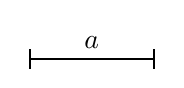
\begin{tikzpicture}[>=latex, scale=1]
\tkzDefPoints{0/0/O, 2.6/0/O', 1/0/P}
\tkzDrawCircles[thick](O,P O',P)
\tkzDrawSegments[thick](O,O')
\tkzLabelPoints[above right](P)
\tkzLabelPoints[below](O,O')
\tkzDrawPoints(O,O')
\draw[|-|, thick](-.6,1.8)--node[above]{$a$}(1,1.8);
  \end{tikzpicture}
  \caption{}
  \end{minipage}
\end{figure}

\begin{example}
已知:$\odot(O,r)$上一点$P$,和线段$a$(图4.24).

求作:一圆使它的半径等于$a$,且与$\odot(O,r)$在$P$点外切.

作法
\begin{enumerate}
\item 作半径$\overline{OP}$,
\item 在射线$OP$上截$\overline{PO'}=a$,
\item 以$O'$为圆心.为半径长,画$\odot O'$,则$\odot O'$为所
求作的圆.
\end{enumerate}
\end{example}

\begin{proof}
  根据作法可知:
\[\overline{OO'}=\overline{OP}+\overline{PO'}=r+a\]

$\therefore\quad \odot O$与$\odot O'$在$P$点外切.
\end{proof}

\begin{ex}
\begin{enumerate}
\item 把本节互逆的两个正确的命题,用“充要”逻辑语句合
写成一个定理.
\item 试说出下列各题中两圆的位置关系:$r$、$r'$分别为两圆的
半径,$d$表示圆心距.
\begin{enumerate}
\item $d=$6cm,\quad $r=$4cm,\quad $r'=$2cm;
\item $d=$2cm,\quad $r=5$cm,\quad $r'=$3cm;
\item $d=$7cm,\quad $r=3$cm,\quad $r'=$2cm;
\item $d=$1cm,\quad $r=6$cm,\quad $ r'=$3cm.
\end{enumerate}

\item 已知两圆外切时,圆心距为12cm,内切时圆心距是4cm,
求两圆的半径的长.
\item 两圆的半径的比是5:3,当两圆外切时,圆心距为24cm,
求这两圆内切时的圆心距.
\item 两个等圆外切,并且它们都内切于另一个大圆,已知这
三个圆的圆心所构成的三角形周长为20cm,求大圆的半
径.
\item 求作一圆,使圆的半径是4cm,并且与已知$\odot (0,2{\rm cm})$
外切于已知点$A$.
\item 求作一圆使圆的半径是2cm,并且与已知$\odot (0,1{\rm cm})$内
切于已知点$P$.
\item 设$\triangle ABC$的三边长分别为7cm,8cm,9cm,试分别以
三顶点为圈心作三个圆两两外切(提示:先计算出三个
圆的半径).
\end{enumerate}
\end{ex}

\subsection{圆与圆的位似}
已知$\odot (O,r)$和一点$S$(图4.25),我们来研究怎样求作$\odot O$的以$S$为位似中心,位似比为常数$k$的位似形.

设$k>0$,由位似变换的定义,我们先作出以$S$点为顺位似中心,$k$为位似比的点$O$的对应点$O'$(图4.25,取$k=\frac{5}{2}$),则
\[\frac{\overline{SO'}}{\overline{SO}}=k\]
\begin{figure}[htp]
  \centering
\begin{tikzpicture}
\tkzDefPoints{0/0/S, 2/0/O, 5/0/O', 2.5/.5/A}
\tkzDefPointWith[linear, K=2.5](S,A)\tkzGetPoint{A'}
\tkzDrawCircles(O,A O',A')
\tkzDrawSegments[thick](O,A O',A')
\tkzDrawLines[add=0 and .15,  thick](S,A')
\tkzDrawLines[add=0 and .5,  thick](S,O')
\tkzLabelPoints[below](O,O')
\tkzLabelPoints[above right](A,A')
\tkzLabelPoints[left](S)
\end{tikzpicture}
  \caption{}
\end{figure}

设$A$是$\odot (O,r)$上任一点,同样可作出$A$的对应点$A'$, 
使$\frac{\overline{SA'}}{\overline{SA}}=k$, 于是
\[\frac{\overline{SO'}}{\overline{SO}}=\frac{\overline{SA'}}{\overline{SA}},\qquad O'A'\parallel OA\]

$\therefore\quad \triangle SO'A'\backsim \triangle SOA$.

\[\frac{\overline{O'A'}}{\overline{OA}}=\frac{\overline{SO'}}{\overline{SO}}=k,\qquad \overline{O'A'}=k\overline{OA}=k\cdot r\]

$\therefore \quad A'$在$\odot (O',kr)$上.

这样,$\odot O$上的每一点,以$S$为顺位似中心,$k$为位似比
的位似点都在$\odot (O',kr)$上.

反过来,如果$A'$点是$\odot (O',kr)$上任一点,我们可求
作一点$A$使$\frac{\overline{SA'}}{\overline{SA}}=k$. 这时$\triangle SO'A'\backsim \triangle SOA$,

$\therefore \quad \frac{\overline{O'A'}}{\overline{OA}}=k$

又$\because\quad \overline{O'A'}=kr$

$\therefore\quad \overline{OA}=r$

$A$点必在$\odot (0,r)$上.

这样,$\odot (O',kr)$上的所有点,又都是以$S$为顺位似
中心,$k$为位似比$\odot (O,r)$上的点的位似点.

由上述正反两方面的说明,$\odot (O,r)$的以$S$为位似中
心,$k$为位似比的位似形是$\odot (O',kr)$.

如给出的常数$k<0$, 与$k>0$的情况类似,我们可作出
已知$\odot (O,r)$的逆位似形(图4.26),这时变换的方向是相
反的,即$O$点的逆位似点$O'$在射线$SO$的反向延长线上,
$A$点的逆位似点在射线$SA$的反向延长线上,$\odot (O',|k|r)$就
是$\odot (O,r)$的逆位似形.

\begin{figure}[htp]
    \centering
  \begin{tikzpicture}[scale=.8]
  \tkzDefPoints{2/0/S, 0/0/O, 5/0/O', 6/2/A'}
  \tkzDefPointsBy[translation= from O' to A'](O){A''}
  \tkzInterLL(O,A'')(A',S)\tkzGetPoint{A}
  \tkzDrawSegments[thick](O,A O',A' A,A')
  \tkzDrawLines[add=.5 and .7, thick](O,O')
  \tkzDrawCircles(O,A O',A')
  \tkzLabelPoints[below](O',A)
  \tkzLabelPoints[above](O,A',S)
  \end{tikzpicture}
    \caption{}
  \end{figure}



综合以上讨论,我们得到:
\begin{blk}{}
    圆的位似形仍是圆.
\end{blk}

进一步我们还可证明:

\begin{blk}{}
任何两个不等的圆,都是位似形,它们即可看作顺位似
形,又可看作逆位似形,它们有两个位似中心.
\end{blk}

已知$\odot (O,r)$和$\odot (O',r')$且$r<r'$(图4.25),我们作
两圆的半径$\overline{OA}$和$\overline{O'A'}$, 且使射线$OA$与$O'A'$的方向相
同,设直线$AA'$与连心线$OO'$交于一点$S$, 这时$S$点在$\overline{O'O}$
的延长线上,于是,
\[\frac{\overline{SO'}}{\overline{SO}}=\frac{r'}{r}\]

由于圆的位似形仍是圆,我们以$S$为位似中心,$\frac{r'}{r}$
为
位似比作$\odot (O,r)$的位似圆$\odot (O',r'')$,则
\[\frac{r''}{r}=\frac{r'}{r}\quad \Rightarrow\quad r''=r'\]
$\odot (O',r'')$就是$\odot (O',r')$.

这就证明了$\odot (O',r')$与$\odot (O,r)$为顺位似形,且位似
比等于它们的半径的比,并且位似中心在它们的连心线上.
如果作两圆的半径$\overline{O'A'}$和$\overline{OA}$, 且使射线$O'A'$与$OA$
的方向相反(图4.26).设$\overline{AA'}$与$\overline{OO'}$相交于$S$, 用同样的方
法也可以证明$\odot (O,r)$与$\odot (O',r')$是以$S$点为逆位似中
心的逆位似图形.

从上述证明过程,我们还可看出,如果两圆相等且不同
心,它们只能看作逆位似图形.

由于凡位似形都是相似形,这样我们也就证明了\textbf{任何两
个圆都是相似形}.

\begin{ex}
\begin{enumerate}
    \item 在图中$S$为$\odot O$和$\odot O'$的顺位似中心,试在$O'$上找
    出以$S$为中心的$A$、$B$、$C$、$D$、$E$、$F$各点的顺位似点.
    \item 求作相离、相交的两个不等的圆的顺位似中心.
    \item 求作相交两圆的逆位似中心.
    \item 求证:如果两圆外切,切点是两圆的逆位似中心;如果
    两圆内切,切点是两圆的顺位似中心.
    \item 两个同心圆的顺位似中心是那一点,逆位似中心呢?
\end{enumerate}
\end{ex}

\begin{figure}[htp]
    \centering
\begin{tikzpicture}[scale=.9]
\tkzDefPoints{-1/0/S, 2/0/a, 3/0/O, 5/0/b, 7/0/O'}
\tkzDrawCircles[thick](O,a O',b)
\tkzDrawLines[add=0 and .3](S,O')
\tkzDefPoint(20:1){c}
\tkzDefPoint(8:1){d}
\tkzDefPoint(-20:1){e}
\tkzInterLC(S,c)(O,a)  \tkzGetPoints{A}{B}
\tkzInterLC(S,c)(O',b)  \tkzGetPoints{P}{Q}
\tkzInterLC(S,d)(O,a)  \tkzGetPoints{C}{D}
\tkzInterLC(S,d)(O',b)  \tkzGetPoints{R}{S'}
\tkzInterLC(S,e)(O,a)  \tkzGetPoints{F}{E}
\tkzInterLC(S,e)(O',b)  \tkzGetPoints{H}{G}
\tkzAutoLabelPoints[center=O](C,D)
\tkzAutoLabelPoints[center=O'](R,S')
\tkzLabelPoints[below](O,O',E,F,G,H)
\tkzLabelPoints[left](S)
\tkzDrawSegments(S,Q S,S' S,H)
\tkzLabelPoints[above](A,B,P,Q)
\tkzDrawPoints(O,O')
\end{tikzpicture}
    \caption*{第1题}
\end{figure}

\section*{习题4.1}
\addcontentsline{toc}{subsection}{习题4.1}
\begin{enumerate}
\item 以$\odot O$的半径$\overline{OA}$为一边作正方形$OABC$, 求证$B$点在
圆外,$C$点在圆上,两条对角线的交点$D$在$\odot O$内.
\item 已知$O$是矩形$ABCD$的对角线的交点,求证$A$、$B$、
$C$、$D$四个顶点在以$O$为圆心,以$OA$为半径的圆上.
\item 已知$AB$、$CD$是$\odot O$中互相垂直的弦,并且$\overline{AB}$把$\overline{CD}$分
成3cm和7cm的两部分,求弦$\overline{AB}$的长和它的弦心距.
\item 经过圆内一个已知点作一条弦,使这条弦被这点所平
分.
\item 已知$\overline{AB}$是$\odot O$的直径,$\overline{CD}$是$\odot O$的弦,$AE\bot $直线$CD$
于$E$点,$BF\bot $直线$CD$于$F$点,求证:$\overline{EC}=\overline{DF}$.
\item 已知$\overline{AB}$是$\odot O$的直径,$\wideparen{AC}$与
$\wideparen{AD}$
位于$\wideparen{AB}$的两侧且
$\wideparen{AC}=\wideparen{AD}$. 求证:$AB$平分$\angle CAD$.
\item 已知$\odot O_1$和$\odot O_2$是相离的两个等圆,一条与连心线$O_1O_2$
平行的直线顺次与$\odot O_1$、$\odot O_2$相交于$A$、$B$、$C$、$D$各
点.求证:$\overline{AB}=\overline{CD}$, $\overline{AB}=\overline{CD}$.
\item 已知$\odot O_1$和$\odot O_2$是相离的两个等圆,过$\overline{O_1O_2}$的中点,作直线顺次与$\odot O_1$、$\odot O_2$相交于$C$、$D$、$E$、$F$各点,求证:
$\wideparen{CD}=\wideparen{EF}$.
\item 在第7题、第8题中,如果条件是相交的两个等圆,结
论是否都还成立.
\item 已知两圆相交,经过它们的一个交点有一条和公共弦垂
直的直线,和两圆相交于另外两点,求证这两点间的
长等于圆心距的2倍.
\end{enumerate}

\section{圆与直线的位置关系}
\subsection{圆与直线的位置关系}
在图4.27中,如果直线$AB$和$\odot O$的圆心$O$的距离$\overline{OD}$大
于半径$\overline{OC}$, 那么$D$点在圆外;在直线${AB}$上再任取一点$M$, 
那么$\overline{OM}>\overline{OD}>\overline{OC}$, 那么$M$点也一定在圆外,所以直线
$AB$上任何一点都在圆外,于是$\odot O$和直线$AB$便没有公共
点.

如果一条直线和一个圆没有公共点,我们就说这条直线
和这个圆\textbf{相离}.

\begin{figure}[htp]\centering
    \begin{minipage}[t]{0.48\textwidth}
    \centering
  \begin{tikzpicture}[>=latex, scale=1]
\tkzDefPoints{-2/0/A, -1/0/M, 0/0/D, 1/0/B, 0/2/O, 0/.5/C}
\tkzDrawLines[add=0 and .3, thick](A,B)
\tkzDrawCircle[thick](O,C)
\tkzDrawSegments[thick](O,M O,D)
\tkzMarkRightAngles[size=.2](O,D,M)
\tkzLabelPoints[below](A,B,D,M)
\tkzLabelPoints[above](O)
\tkzLabelPoints[above right](C)
\tkzDrawPoints(A,B,D,M,O,C)
    \end{tikzpicture}
    \caption{}
    \end{minipage}
    \begin{minipage}[t]{0.48\textwidth}
    \centering
    \begin{tikzpicture}[>=latex, scale=1]
\tkzDefPoints{0/0/O, .5/2.5/a, 2/-1.5/b}
\tkzDefPointBy[projection = onto a--b](O)\tkzGetPoint{A}
\tkzDrawCircle[thick](O,A)
\tkzDefPointWith[linear, K=.8](a,b) \tkzGetPoint{P}
\tkzDefPointWith[linear, K=.95](a,b) \tkzGetPoint{B}
\tkzDrawSegments[thick](a,b O,A O,P)
\tkzMarkRightAngles[size=.2](O,A,a)
\tkzLabelPoints[right](A,P,B)
\tkzLabelPoints[left](O)

    \end{tikzpicture}
    \caption{}
    \end{minipage}
    \end{figure}

在图4.28中,过$\odot (O,r)$的任一条半径$\overline{OA}$的端点$A$作直
线$AB\bot \overline{OA}$于$A$点,$P$为直线$AB$上除$A$点外的任一点,则
$\overline{OP}>\overline{OA}$, 于是$P$就在圆外,这就是说,在直线$AB$上,除$A$点外其它的点都在圆外.这时直线$AB$和$\odot O$只有一个公共
点$A$.

如果一条直线和一个圆只有一个公共点,我们就说这条
直线和这个圆\textbf{相切},这条直线叫做圆的\textbf{切线},这个公共点叫
做它们的切点.

\begin{blk}
    {切线判定定理} 经过圆的半径外端,并且垂直这条半径
的直线是这圆的切线.
\end{blk}

这就是说,“一条直线经过半径外端且垂直于半径”为
这条直线是圆的切线的充分条件,反过来可证条件也是必要
的.

\begin{blk}
    {切线性质定理} 圆的切线垂直于经过切点的半径.
\end{blk}

已知:直线$AB$与$\odot O$相
切于$C$点(图4.29).

求证:$AB\bot \overline{OC}$.

\begin{proof}
    假设$AB$和$\overline{OC}$不垂
直,自圆心$O$引$\overline{OD}\bot AB$于$D$
点,在$AB$上取$\overline{DC'}=\overline{DC}$, 且
使$D$点在$C$与$C'$之间,于是
$OD$垂直平分$\overline{CC'}$, $\overline{OC'}=\overline{OC}$.

$\because\quad C$点是切点,$\overline{OC}$是$O$的半径.

$\therefore\quad \overline{OC'}$是$O$的半径,$C'$点也在$\odot O$上.

这就是说,直线$AB$和$\odot O$有了两个公共点$C$和$C'$,但
这与$AB$是圆的切线,即$AB$和$\odot O$只有一个公共点相矛
盾,

$\therefore\quad AB\bot \overline{OC}$.
\end{proof}

\begin{figure}[htp]\centering
    \begin{minipage}[t]{0.48\textwidth}
    \centering
  \begin{tikzpicture}[>=latex, scale=1]
\tkzDefPoints{-1/0/A, 1.5/0/C, 2/0/D, 3/0/C', 4/0/B, 1.5/1.5/O}
\tkzDrawCircle[thick](O,C)
\tkzDrawSegments[thick](A,B C,O C',O D,O)
\tkzLabelPoints[above](O)
\tkzLabelPoints[below](A,B,C,D,C')
    \end{tikzpicture}
    \caption{}
    \end{minipage}
    \begin{minipage}[t]{0.48\textwidth}
    \centering
    \begin{tikzpicture}[>=latex, scale=1.2]
\tkzDefPoints{-2/0/a, -1/0/A, 1/0/A', 2/0/B, 0/1/O, 0/0/D}
\tkzDrawCircle[thick](O,A)
\tkzDrawSegments[thick](B,a O,D)
\tkzLabelPoints[below](A,A',B,D)
\tkzLabelPoints[above](O)
\tkzMarkRightAngles[size=.2](O,D,A')
    \end{tikzpicture}
    \caption{}
    \end{minipage}
    \end{figure}


在图4.30中,经过半径$\overline{OA}$的端点$A$, 作与$\overline{OA}$不垂直
的任一条直线$AB$, 由上面的证明可知:这条直线和圆不能
只有一个公共点,还必须有另一个交点$A'$. 这就是说,直
线$AB$和$\odot O$有了两个公共点.

如果一条直线和一个圆有
两个公共点,我们就说,这条
直线和这个圆相交,这条直线叫做这个圆的\textbf{割线},这两个公
共点叫做它们的\textbf{交点}.

一条直线和一个圆如果有公共点,那么,它们的公共点
是不能多于两个的,因此,\textbf{直线和圆的位置关
系只能有相离、相切和相交三种关系}.





\begin{example}
    求证连结圆的两条平切线的切点间的弦必是圆
的直径.

已知:直线$\ell_1$和直线$\ell_2$分别与$\odot O$切于$A$、$B$两点,且$\ell_1\parallel \ell_2$.

求证:$\overline{AB}$是$\odot O$的直径.
\end{example}

\begin{figure}[htp]
    \centering
\begin{tikzpicture}
\tkzDefPoints{-2/0/a, 2/0/b, -2/1/a', -2/-1/a'', 0/0/O, 1/0/o}
\tkzDefPointsBy[translation= from a to b](a',a''){b',b''}
\tkzDrawSegments[thick](a,b a',b' a'',b'')
\tkzLabelPoint[right](b'){$\ell_1$}
\tkzLabelPoint[right](b''){$\ell_2$}
\tkzLabelPoint[right](b){$\ell_3$}
\tkzDrawCircle[thick](O,o)
\tkzLabelPoints[below right](O)
\tkzDefPoints{0/1/A,0/-1/B}
\tkzDrawSegments[thick](A,B)
\tkzLabelPoints[above](A)
\tkzLabelPoints[below](B)
\tkzLabelPoint[above left](O){1}
\tkzLabelPoint[below left](O){2}


\end{tikzpicture}
    \caption{}
\end{figure}

\begin{proof}
    作$\overline{OA}$、$\overline{OB}$, 过$O$
点作直线$\ell_3\parallel \ell_2$

$\because\quad \ell_1\parallel \ell_2$

$\therefore\quad \ell_3\parallel \ell_1$

$\because\quad \ell_1$是$\odot O$的切线,

$\therefore\quad \overline{OA}\bot \ell_1,\quad \overline{OA}\bot \ell_3,\quad \angle 1=90^{\circ}$
同理可证:$\angle 2=90^{\circ}$.

$\therefore\quad \angle 1+\angle 2=180^{\circ}$.

$\therefore\quad A$、$O$、$B$三点共线.即$\overline{AB}$通过圆心$O$, $\overline{AB}$是$\odot O$的
直径.
\end{proof}


利用例4.10所证原理,早在公元九年,我国就已发明出一
种可以测量圆形工件直径的卡尺.这种卡尺是青铜制的,由
两支丁字形具有刻度的尺子所组成(图4.32),这是世界上
最早的卡尺.由于当时是王莽称帝时代(公元9—23年,王莽
称帝,国号新)后人多把这种卡尺叫做《王莽卡尺》.
\begin{figure}[htp]
    \centering
\includegraphics[scale=.7]{fig/4-32.png}
    \caption{}
\end{figure}

\begin{example}
    已知:$P$点在已知$\odot O$外(图4.33).

求作:经过$P$点的$\odot O$的切线.

作法
\begin{enumerate}
    \item 作$\overline{OP}$
    \item 以$\overline{OP}$的中点$C$为圆
心,以$\overline{CO}$为半径作$\odot C$交$\odot O$于$A$、$B$两点;
\item 作直线$PA$、$PB$, 则$PA$、$PB$就是所求作的切线.
\end{enumerate}
\end{example}

\begin{figure}[htp]
    \centering
\begin{tikzpicture}[scale=.8]
\tkzDefPoints{0/0/O, 5/0/P, 1.5/0/a}
\tkzDefMidPoint(O,P)\tkzGetPoint{C}
\tkzDrawCircle[thick](O,a)
\tkzDrawCircle[dashed](C,O)
\tkzInterCC(O,a)(C,O)  \tkzGetPoints{A}{B}
\tkzDrawLines[very thick](A,P B,P)
\tkzLabelPoints[above](A)
\tkzLabelPoints[above right](P)
\tkzLabelPoints[below](B,C)
\tkzLabelPoints[left](O)
\tkzDrawSegments[dashed](O,P A,C A,O)
\tkzLabelAngle[pos=1.5](C,A,P){1}
\tkzLabelAngle[pos=1.5](A,P,C){2}
\tkzLabelAngle[pos=.5](O,A,C){3}
\tkzLabelAngle[pos=.5](C,O,A){4}

\end{tikzpicture}
    \caption{}
\end{figure}



\begin{proof}
  作$\overline{OA}$、$\overline{CA}$.

$\because\quad  \overline{CA}=\overline{CO}=\overline{CP}$,

$\therefore\quad \angle 1=\angle 2,\quad \angle 3=\angle 4,\quad \angle 1+\angle 3=\angle 2+\angle 4$.

$\because\quad \angle 1+\angle 3+\angle 2+\angle 4=180^{\circ}$,

$\therefore\quad \angle 1+\angle 3=90^{\circ}$, 即$OA\bot PA$,
$PA$是$\odot O$的切线(切线判定定理).

同理可证$PB$也是所求作的切线.

另外,在直角$\triangle POA$和直角$\triangle POB$中,

$\because\quad \overline{OA}=\overline{OB},\quad \overline{PO}=\overline{PO}$.

$\therefore\quad \triangle POA\cong \triangle POB,\quad 
\overline{PA}=\overline{PB}$.  
\end{proof}

如果$\overline{PA}$, $\overline{PB}$的长叫做$P$点到圆的切线长,那么我们就可得到下面的定理:

\begin{blk}
    {切线长定理}
从圆外一个已知点到圆的两条切线的长相
等.
\end{blk}

以$\triangle POA\cong \triangle POB$, 还可推出$\angle APO=\angle BPO$, 因此又
可得出:

\begin{blk}
    {定理} 连结圆外一个已知点和圆心的直线,平分从这点
向圆所作的两条切线所夹的角.
\end{blk}

\begin{ex}
\begin{enumerate}
    \item 回答如下问题.
\begin{enumerate}
    \item 设$\odot (O,r)$的圆心$O$点和直线$\ell$的距离为$d$, 试分
    别说出$d>r$, $d=r$, $d<r$时,直线$\ell$和$\odot (O,r)$的位置关系.
    \item 凡是和圆的一条半径垂直的直线,都是圆的切线
    吗?凡是经过半径外端的直线都是圆的切线吗?
\end{enumerate}
    \item 过圆上一点作圆的切线.
    \item 作一圆与已知直线相切于直线上已知点,这样的圆可作
    多少?这些圆的圆心组成什么图形?
    \item $PA$、$PB$都是$\odot O$的切线,$A$、$B$是切点,求证:
    $\angle AOB+\angle APB=180^{\circ}$.
    \item 求证经过圆的直径两端的两条切线互相平行.
    \item 在已知圆内画两条互相垂直的直径,经过各直径的端点
    画圆的切线;问这四条切线相交成什么四边形?为什
    么?
    \item 从圆外一点向圆作两条切线.求证;连结这点和圆心的
    直线垂直平分连结两切点的线段.
\end{enumerate}
\end{ex}

\subsection{三角形的内切圆}
如果一个多边形的各边都和一个圆相切(图4.34),这
个多边形叫做\textbf{圆的外切多边形},这个圆叫做多边形的\textbf{内切
圆},内切圆的圆心又叫做外切多边形的\textbf{内心}.如图4.34所
示,$ABCD$是$\odot O$的外切四边形,$ABCDE$是$\odot P$的外切五
边形等,$O$、$P$分别是四边形$ABCD$与五边形$ABCDE$
的内心.

\begin{figure}[htp]
    \centering
  \begin{tikzpicture}[scale=.8]
    \begin{scope}
  \tkzDefPoints{0/0/O,1.5/0/a}
  \tkzDefPoint(80:1.5){b}
  \tkzDefPoint(170:1.5){c}
  \tkzDefPoint(-90:1.5){d}
  \tkzDrawCircle[thick](O,a)
  \tkzLabelPoints[below](O)
  \tkzDrawPoints(O)
  \tkzDefTangent[at=a](O) \tkzGetPoint{a'}
  \tkzDefTangent[at=b](O) \tkzGetPoint{b'}
  \tkzDefTangent[at=c](O) \tkzGetPoint{c'}
  \tkzDefTangent[at=d](O) \tkzGetPoint{d'}
  \tkzInterLL(a,a')(b,b')\tkzGetPoint{C}
  \tkzInterLL(c,c')(b,b')\tkzGetPoint{D}
  \tkzInterLL(c,c')(d,d')\tkzGetPoint{A}
  \tkzInterLL(a,a')(d,d')\tkzGetPoint{B}
  \tkzDrawPolygon[thick](A,B,C,D)
  \tkzAutoLabelPoints[center=O](A,B,C,D)
    \end{scope}
    \begin{scope}[xshift=5cm]
    \tkzDefPoints{0/0/P}
  \tkzDefPoint(0:1.5){a}
  \tkzDefPoint(70:1.5){b}
  \tkzDefPoint(150:1.5){c}
  \tkzDefPoint(-145:1.5){d}
  \tkzDefPoint(-80:1.5){e}
  \tkzDrawCircle[thick](P,a)
  \tkzLabelPoints[below](P)
  \tkzDrawPoints(P)
  \tkzDefTangent[at=a](P) \tkzGetPoint{a'}
  \tkzDefTangent[at=b](P) \tkzGetPoint{b'}
  \tkzDefTangent[at=c](P) \tkzGetPoint{c'}
  \tkzDefTangent[at=d](P) \tkzGetPoint{d'}
  \tkzDefTangent[at=e](P) \tkzGetPoint{e'}
  \tkzInterLL(a,a')(b,b')\tkzGetPoint{C}
  \tkzInterLL(c,c')(b,b')\tkzGetPoint{D}
  \tkzInterLL(c,c')(d,d')\tkzGetPoint{E}
  \tkzInterLL(e,e')(d,d')\tkzGetPoint{A}
  \tkzInterLL(a,a')(e,e')\tkzGetPoint{B}
  \tkzDrawPolygon[thick](A,B,C,D,E)
  \tkzAutoLabelPoints[center=P](A,B,C,D,E)
    \end{scope}
    \begin{scope}[xshift=10cm]
    \tkzDefPoints{0/0/Q,1.5/0/a}
  \tkzDefPoint(58:1.5){b}
  \tkzDefPoint(125:1.5){c}
  \tkzDefPoint(170:1.5){d}
  \tkzDefPoint(-125:1.5){e}
  \tkzDefPoint(-68:1.5){f}
  \tkzDrawCircle[thick](Q,a)
  \tkzLabelPoints[below](Q)
  \tkzDrawPoints(Q)
  \tkzDefTangent[at=a](Q) \tkzGetPoint{a'}
  \tkzDefTangent[at=b](Q) \tkzGetPoint{b'}
  \tkzDefTangent[at=c](Q) \tkzGetPoint{c'}
  \tkzDefTangent[at=d](Q) \tkzGetPoint{d'}
  \tkzDefTangent[at=e](Q) \tkzGetPoint{e'}
  \tkzDefTangent[at=f](Q) \tkzGetPoint{f'}
  \tkzInterLL(a,a')(b,b')\tkzGetPoint{C}
  \tkzInterLL(c,c')(b,b')\tkzGetPoint{D}
  \tkzInterLL(c,c')(d,d')\tkzGetPoint{E}
  \tkzInterLL(e,e')(d,d')\tkzGetPoint{F}
  \tkzInterLL(e,e')(f,f')\tkzGetPoint{A}
  \tkzInterLL(a,a')(f,f')\tkzGetPoint{B}
  \tkzDrawPolygon[thick](A,B,C,D,E,F)
  \tkzAutoLabelPoints[center=Q](A,B,C,D,E,F)
    \end{scope}
  \end{tikzpicture}
    \caption{}
  \end{figure}

已知$\odot I$, 过这圆上$D$、
$E$、$F$三点作它的三条切线交成
$\triangle ABC$(图4.35), 于是$\odot I$
便是$\triangle ABC$的内切圆.由于切
线垂直于过切点的半径,则内
心$I$到三边的距离相等,$I$在
$\triangle ABC$的三个内角的平分线上.


  \begin{figure}[htp]\centering
    \begin{minipage}[t]{0.48\textwidth}
    \centering
  \begin{tikzpicture}[>=latex, scale=.7]
\tkzDefPoints{0/0/I}
  \tkzDefPoint(15:1.5){E}
  \tkzDefPoint(135:1.5){F}
  \tkzDefPoint(-90:1.5){D}
  \tkzLabelPoints[above](I)
  \tkzDefTangent[at=E](I) \tkzGetPoint{a'}
  \tkzDefTangent[at=F](I) \tkzGetPoint{b'}
  \tkzDefTangent[at=D](I) \tkzGetPoint{c'}
  \tkzInterLL(E,a')(F,b')\tkzGetPoint{A}
  \tkzInterLL(D,c')(F,b')\tkzGetPoint{B}
  \tkzInterLL(D,c')(E,a')\tkzGetPoint{C}
  \tkzLabelPoints[below](B,D,C)
  \tkzLabelPoints[above](A)
  \tkzLabelPoints[left](F)
  \tkzLabelPoints[right](E)
  \tkzDrawPolygon[thick](A,B,C)
  \tkzDrawSegments[dashed](B,I C,I A,I)
  \tkzDrawSegments[thick](I,F I,D I,E)
  \tkzDrawCircle[thick](I,E)
    \end{tikzpicture}
    \caption{}
    \end{minipage}
    \begin{minipage}[t]{0.48\textwidth}
    \centering
    \begin{tikzpicture}[>=latex, scale=.8]
\tkzDefPoints{0/0/B, .8/1.5/A, 2/-.1/C}
    \tkzDefSpcTriangle[excentral,name=I](A,B,C){_1,_2,_3}
    \tkzDefSpcTriangle[extouch,name=T](A,B,C){_1,_2,_3}
    \tkzDrawPolygon[thick](I_1,I_2,I_3)
    \tkzLabelPoints[above](A)
    \tkzLabelPoints[below left](B)
    \tkzLabelPoints[below right](C)
    \tkzLabelPoints[above right](I_2)
    \tkzLabelPoints[below](I_1)
    \tkzLabelPoints[above left](I_3)
    \tkzDrawCircles(I_1,T_1 I_2,T_2 I_3,T_3)
  
  \tkzDrawLines[add=1.3 and 1.3, thick](A,C B,C A,B)
  \tkzDrawSegments(A,I_1 B,I_2 C,I_3)
  \tkzInterLL(A,I_1)(B,I_2)\tkzGetPoint{I}
    \tkzLabelPoints[above right](I)
    \end{tikzpicture}
    \caption{}
    \end{minipage}
    \end{figure}


  仿此,我们还可证明:
  三角形一内角平分线和其余两内角的外角平分线交于一点,这一点叫做三角形的\textbf{旁心}(图4.36),以旁心为圆心可作一圆和一边及其它两边的延长线相切、所作的圆叫做三角形的\textbf{旁切圆},一个三角形有三个旁心,三个旁切圆,如图4.36所示,$\odot I_1$、$\odot I_2$、$\odot I_3$是$\triangle ABC$的三个旁切圆.
  
  \begin{example}
  已知$\triangle ABC$,$\overline{BC}=a$、$\overline{AC}=b$,$\overline{AB}=c$,求三个顶点到内切圆的切线长(图4.37).
  \end{example}
  
  \begin{solution}
    设$\triangle ABC$的三边、$\overline{BC}$、$\overline{CA}$、$\overline{AB}$分别与内切圆$I$
  相切于$D$、$E$、$F$三点,由于从圆外一点引圆的两条切线长相等,
  
  $\therefore\quad \overline{AE}=\overline{AF},\quad \overline{BF}=\overline{BD},\quad \overline{CD}=\overline{CE}$. 
  
  设$\overline{AE}=x$、$\overline{BF}=y$,$\overline{CD}=z$,则可得到,
  \[\begin{cases}
    x+y=c\\
    y+z=a\\
    z+x=b
  \end{cases}\]
  解之得:
  \[x=\frac{b+c-a}{2},\quad y=\frac{a+c-b}{2},\quad z=\frac{a+b-c}{2}\]
  
  答:三个顶点$A$、$B$、$C$到内切圆的切线长分别为
  \[\frac{b+c-a}{2},\qquad \frac{a+c-b}{2},\qquad \frac{a+b-c}{2}\]
  \end{solution}
  
  \begin{figure}[htp]
    \centering
    \begin{minipage}[t]{0.48\textwidth}
    \centering
    \begin{tikzpicture}[>=latex, scale=.7]
  \tkzDefPoints{0/0/I}\tkzDrawPoints(I)
  \tkzDefPoint(15:1.5){E}
  \tkzDefPoint(135:1.5){F}
  \tkzDefPoint(-90:1.5){D}
  \tkzLabelPoints[right](I)
  \tkzDefTangent[at=E](I) \tkzGetPoint{a'}
  \tkzDefTangent[at=F](I) \tkzGetPoint{b'}
  \tkzDefTangent[at=D](I) \tkzGetPoint{c'}
  \tkzInterLL(E,a')(F,b')\tkzGetPoint{A}
  \tkzInterLL(D,c')(F,b')\tkzGetPoint{B}
  \tkzInterLL(D,c')(E,a')\tkzGetPoint{C}
  \tkzLabelPoints[below](B,D,C)
  \tkzLabelPoints[above](A)
  \tkzLabelPoints[left](F)
  \tkzLabelPoints[right](E)
  \tkzDrawPolygon[thick](A,B,C)
  \tkzDrawCircle[thick](I,E)
  \tkzLabelSegment[below](B,D){$y$}
  \tkzLabelSegment[below](C,D){$z$}
  \tkzLabelSegment[left](B,F){$y$}
  \tkzLabelSegment[left](A,F){$x$}
  \tkzLabelSegment[right](A,E){$x$}
  \tkzLabelSegment[right](E,C){$z$}
  
  
    \end{tikzpicture}
    \caption{}
    \end{minipage}
    \begin{minipage}[t]{0.48\textwidth}
    \centering
    \begin{tikzpicture}[>=latex, scale=1]
  \tkzDefPoints{0/0/I}
  \tkzDefPoint(0:1){E}
  \tkzDefPoint(135:1){F}
  \tkzDefPoint(-90:1){D}
  \tkzLabelPoints[above](I)
  \tkzDefTangent[at=E](I) \tkzGetPoint{a'}
  \tkzDefTangent[at=F](I) \tkzGetPoint{b'}
  \tkzDefTangent[at=D](I) \tkzGetPoint{c'}
  \tkzInterLL(E,a')(F,b')\tkzGetPoint{A}
  \tkzInterLL(D,c')(F,b')\tkzGetPoint{B}
  \tkzInterLL(D,c')(E,a')\tkzGetPoint{C}
  \tkzLabelPoints[below](B,C)
  \tkzLabelPoints[above](A)
  \tkzDrawPolygon[thick](A,B,C)
  \tkzDrawCircle[thick](I,E)
  \tkzDrawSegments[thick](I,E I,F I,D)
  \tkzDrawSegments[dashed](A,I B,I C,I)
  \tkzLabelSegment[above](I,E){$r$}
  \tkzLabelSegment[below](I,F){$r$}
  \tkzLabelSegment[right](I,D){$r$}
  
    \end{tikzpicture}
    \caption{}
    \end{minipage}
  \end{figure}
  
  \begin{example}
  在直角$\triangle ABC$中,$\angle C=90^{\circ}$, $\overline{AB}=3$cm, $\overline{AC}=2$cm.
  
  求:直角三角形内切圆半径长(图4.38).
  \end{example}
  
  \begin{solution}
    设$\odot I$为$\triangle ABC$的内切圆,半径为$r$.
  
  $\because\quad \triangle AIB$的面积$+\triangle BIC$的面积$+\triangle AIC$的面积$=\triangle ABC$的面积
  
  $\therefore\quad r\x \overline{AB}+r\x \overline{BC}+r\x \overline{AC}=\overline{AC}\x \overline{BC}$
  
  又知:$\overline{AB}=3,\quad \overline{AC}=2,\quad \overline{BC}=\sqrt{3^2-2^2}=\sqrt{5}$
  
  $\therefore\quad r\x 3+r\x \sqrt{5}+r\x 2=2\x \sqrt{5}$
  
  \[r=\frac{2\sqrt{5}}{5+\sqrt{5}}=\frac{10\sqrt{5}-10}{20}=\frac{\sqrt{5}-1}{2}\]
  
  答:内切圆半径等于$\frac{\sqrt{5}-1}{2}$cm.
  \end{solution}

\begin{ex}
\begin{enumerate}
    \item 求作一个三角形的内切圆.
    \item 求作一个三角形的三个旁切圆.
    \item 在$\triangle ABC$中,$\overline{BC}=28$cm, $\overline{AC}=18$cm, $\overline{AB}=26$cm, 它的内
    切圆分别和$\overline{BC}$, $\overline{AC}$, $\overline{AB}$
    相切于$D$、$E$、$F$, 求$\overline{AF}$、$\overline{BD}$
    和$\overline{CE}$的长.
    \item 已知$\triangle ABC$, $\overline{BC}=a$, $\overline{AC}=b$, $\overline{AB}=c$, 面积是$s$, 求它的
    内切圆半径.
    \item 已知直角三角形的两直角边分别是$a$、$b$, 求这个直角三
    角形的内切圆半径$r$.
\end{enumerate}
\end{ex}

\subsection{圆的外切四边形}

我们已经知道,每一个三角形都有一个内切圆,现在要
问,是不是每个四边形也都有
一个内切圆呢?如果四边形有
一个内切圆,那么,这个四边
形的四个角的平分线应相交于
一点,显然,这个性质并不是
每个四边形都能具备的.下面
先让我们来寻求四边形有内切
圆的必要条件.

\begin{figure}[htp]
    \centering
\begin{tikzpicture}
\tkzDefPoints{0/0/I, 0/-1.5/Q}
\tkzDefPoint(10:1.5){R}
\tkzDefPoint(165:1.5){P}
\tkzDefPoint(75:1.5){S}
\tkzDefTangent[at=R](I) \tkzGetPoint{a}
\tkzDefTangent[at=S](I) \tkzGetPoint{b}
\tkzDefTangent[at=P](I) \tkzGetPoint{c}
\tkzDefTangent[at=Q](I) \tkzGetPoint{d}
\tkzInterLL(R,a)(S,b)\tkzGetPoint{C}
\tkzInterLL(S,b)(P,c)\tkzGetPoint{D}
\tkzInterLL(P,c)(Q,d)\tkzGetPoint{A}
\tkzInterLL(R,a)(Q,d)\tkzGetPoint{B}
\tkzDrawPolygon[thick](A,B,C,D)
\tkzDrawCircle[thick](I,Q)
\tkzLabelPoints[below](A,Q,B)
\tkzLabelPoints[left](D,P)
\tkzLabelPoints[right](C,R,I)
\tkzLabelPoints[above](S)
\tkzDrawPoints(I)
\end{tikzpicture}
    \caption{}
\end{figure}


已知$\odot I$, 过圆上四点$P$、$Q$、$R$、$S$分别作$\odot I$的切线交
成四边形$ABCD$(图4.39). 于是有,
\begin{equation*}
    \overline{AP}=\overline{AQ},\quad \overline{BR}=\overline{BQ},\quad \overline{CR}=\overline{CS},\quad 
\overline{DP}=\overline{DS}\tag{切线长定理}
\end{equation*}
将四个等式左右各相加得:
\[\overline{AP}+\overline{BR}+\overline{CR}+\overline{DP}=\overline{AQ}+\overline{BQ}+\overline{CS}+\overline{DS}\]
即:$\overline{AD}+\overline{BC}=\overline{AB}+\overline{CD}$.

这就说“对边的和相等”是圆外切四边形的一个必要条
件.于是我们得到:

\begin{blk}
    {定理}圆的外切四边形的每双对边的和相等.
\end{blk}

现在要问,“对边的和相等”是不是一个四边形有内切
圆的充分条件呢?答案也是肯定的.

\begin{blk}
    {定理}如果四边形的每双对边的和此相等,则它必有
内切圆.
\end{blk}

已知:在四边形$ABCD$中(图4.40), $\overline{AB}+\overline{CD}=\overline{AD}+\overline{BC}$.

求证:四边形$ABCD$有内切圆.

\begin{figure}[htp]
    \centering
\begin{tikzpicture}
\tkzDefPoint(-90:1.5){E}
\tkzDefPoint(0:1.5){F}
\tkzDefPoint(60:1.5){G}
\tkzDefPoint(150:1.5){H}
\tkzDefPoint(0,0){I}
\tkzDefTangent[at=E](I) \tkzGetPoint{a}
\tkzDefTangent[at=F](I) \tkzGetPoint{b}
\tkzDefTangent[at=G](I) \tkzGetPoint{c}
\tkzDefTangent[at=H](I) \tkzGetPoint{d}
\tkzInterLL(E,a)(F,b)\tkzGetPoint{B}
\tkzInterLL(F,b)(G,c)\tkzGetPoint{C}
\tkzInterLL(G,c)(H,d)\tkzGetPoint{D}
\tkzInterLL(E,a)(H,d)\tkzGetPoint{A}
\tkzDrawPolygon[thick](A,B,C,D)
\tkzDrawCircle[thick](I,E)
\tkzDrawSegments[dashed](I,E I,F I,G I,H I,D A,C B,I)
\tkzAutoLabelPoints[center=I](E,F,G,H,A,B,C,D)
\tkzInterLC(A,B)(B,C)  \tkzGetPoints{M}{M'}
\tkzInterLC(A,D)(D,C)  \tkzGetPoints{N}{N'}
\tkzDrawSegments[thick](M,N)
\tkzLabelPoints[below](M)
\tkzLabelPoints[left](N)
\tkzLabelPoints[above right](I)
\tkzDrawSegments[dashed](C,N C,M)
\end{tikzpicture}
    \caption{}
\end{figure}


\begin{proof}
    假定$\overline{AB}>\overline{BC}$, 则根据已知条件$\overline{AB}+\overline{CD}=\overline{AD}+
    \overline{BC}$, 可知$\overline{AD}>\overline{CD}$. 故在$\overline{AB}$及$\overline{AD}$上,可以截取线段
    $\overline{BM}=\overline{BC}$, $\overline{DN}=\overline{DC}$, 从而,
\[\overline{AM}=\overline{AB}-\overline{BC},\quad \overline{AN}=\overline{AD}-\overline{CD}\]

但根据已知条件$\overline{AB}-\overline{BC}=\overline{AD}-\overline{CD}$, 

$\therefore\quad \overline{AM}=\overline{AN}$.

连结$\overline{MN}$、$\overline{CM}$、$\overline{CN}$, 于是$\triangle AMN$、$\triangle BCM$、$\triangle DCN$都是等
腰三角形,因此它们的顶角$\angle A$、$\angle B$、$\angle C$的平分线,必然
是底边$\overline{MN}$、$\overline{CM}$、$\overline{CN}$的垂直平分线,这样一来,这三条角
平分线也是$\triangle CMN$的边$\overline{MN}$、$\overline{CM}$、$\overline{CN}$的垂直平分线.所
以这三条角平分线一定相交于一点$I$. 自$I$点分别作$\overline{AB}$、$\overline{BC}$、$\overline{CD}$、$\overline{DA}$的垂线,垂足分别是$E$、$F$、$G$、$H$. 于是得
\[\overline{IE}=\overline{IF}=\overline{IG}=\overline{IH}\]

因此,以$I$为圆心,$\overline{IE}$为半径的圆与四边形$ABCD$的
各边分别相切于$E$、$F$、$G$、$H$四点、即四边形有内切圆
$\odot I$. 
\end{proof}

\begin{rmk}
    在证明本定理时,假定了$\overline{AB}>\overline{BC}$, 如果$\overline{AB}<\overline{BC}$, 
证明方法完全一样,如果$\overline{AB}=\overline{BC}$, 那么,证法就更简单了,
请同学们想一想为什么?
\end{rmk}

\begin{ex}
\begin{enumerate}
    \item 一个菱形有内切圆吗?一个正方形呢?如果有,就分别
    作出一个菱形和一个正方形的内切圆.
    \item 作一等边三角形的内切圆和外接圆,内心和外心重合吗?
    \item 果一个四边形的每双对边和不相等,你能否判定这个
    四边形有没有内切圆?为什么?
    \item 如果四边形的各边的比顺次地如下列各数的比
\begin{multicols}{3}
\begin{enumerate}
    \item $2:2:3:3$
    \item $2:5:3:4$
    \item $3:5:3:1$
\end{enumerate}
\end{multicols}
这些四边形是否有内切圆?
\end{enumerate}
\end{ex}

\subsection{两圆的公切线}
如图4.41所示,一条直线与两圆都相切,这条直线就叫
做两圆的公切线.如果两圆的圆心都在公切线的同侧,这条
公切线就叫做两圆的\textbf{外公切线};如果两圆的圆心分别在公切
线的两侧,这条公切线就叫做两圆的\textbf{内公切线}.显然,如果
两圆相交,两圆只有外公切线而无内公切线(图4.41(2)).

\begin{figure}[htp]
    \centering
\begin{tikzpicture}
\begin{scope}
\tkzDefPoints{0/0/O, 1/0/a, 3/0/O', 3-1.2/0/b}
\tkzDrawCircles[thick](O,a O',b)
\tkzDrawPoints(O,O')
\tkzDefPoint(93.82:1){M}
\tkzDefPoint(-93.82:1){M'}
\tkzDefPointsBy[translation= from O to O'](M,M'){N,N'}
\tkzDefTangent[at=M](O) \tkzGetPoint{a}
\tkzDefTangent[at=M'](O) \tkzGetPoint{b}
\tkzInterLL(O',N)(M,a) \tkzGetPoint{P}
\tkzInterLL(O',N')(M',b) \tkzGetPoint{P'}
\tkzDrawLines[add=.5 and .5, thick](M,P M',P')
\tkzDefPoints{1.36/0/T}
\tkzDefPoint(42.67:1){R}
\tkzDefPoint(-42.67:1){R'}
\tkzDrawLines[add=2.5 and 1, thick](T,R T,R')
\node at (1.5,-1.7){(1)};
\end{scope}
\begin{scope}[xshift=7cm]
    \tkzDefPoints{0/0/O, 1/0/a, 1.5/0/O', 1.5-1.2/0/b}
\tkzDrawPoints(O,O')
\tkzDrawCircles[thick](O,a O',b) 
\tkzDefPoint(97.66:1){M}
\tkzDefPoint(-97.66:1){M'}
\tkzDefPointsBy[translation= from O to O'](M,M'){N,N'}
\tkzDefTangent[at=M](O) \tkzGetPoint{a}
\tkzDefTangent[at=M'](O) \tkzGetPoint{b}
\tkzInterLL(O',N)(M,a) \tkzGetPoint{P}
\tkzInterLL(O',N')(M',b) \tkzGetPoint{P'}
\tkzDrawLines[add=1 and 1, thick](M,P M',P')
\node at (.75,-1.7){(2)};

\end{scope}
\end{tikzpicture}
    \caption{}
\end{figure}



一条公切线上两切点间线段的长,叫做两圆的公切线的
长.

在实践中,要画两圆的公切线时,可将直尺渐渐移动使
靠近两圆直至和两圆各只有一个接触点时,然后沿着直尺的
边缘,就可画出两圆的公切线.

下面我们来研究只用圆规和直尺两圆外公切线的方
法.

\subsubsection{作两个圆的外公切线}

已知:$\odot(O,r)$和$\odot (O',r')$且$r>r'$.

求作:$\odot O$和$\odot O'$的外公切线.

\begin{figure}[htp]
  \centering
\begin{tikzpicture}[scale=.8]
\tkzDefPoints{0/2/A, 5/2/B, 0/.8/E, 5/.8/O', 0/0/O}
\tkzDrawCircles(O,E O,A O',B)
\tkzDrawLines[thick](A,B)
\tkzDrawLines[thick, add=0 and .2](O',E)
\tkzLabelPoints[above](A,B)
\tkzDrawSegments[thick](B,O')
\tkzLabelPoints[below](O,O')
\tkzDrawSegments(A,O)
\tkzLabelPoints[above right](E)
\end{tikzpicture}
  \caption{}
\end{figure}


\begin{analyze}
  假设$AB$是所求作的$\odot O$和$\odot O$的外公切线(图4.42),$A$和$B$是切点,分别作半径$\overline{OA}$,$\overline{O'B}$,由于$\overline{OA}$,$\overline{O'B}$都垂直于$AB$,所以$OA\parallel O'B$,作$O'E\parallel AB$交$\overline{OA}$于$E$点,则$O'E\bot OA$,且$\overline{OE}=r-r'$,这时$O'E$与$\odot (O,r-r')$相切于$E$点.$\odot (O,r-r')$可作,过$O'$也可作$\odot (O,r-r')$的切线.故切点$E$可定,于是$AB$可作.
\end{analyze}

作法(图4.43).
\begin{enumerate}
\item 作$\odot (O,r-r')$;
\item 从$O'$点作$\odot (O,r-r')$的切线$O'E$,$E$为切点;
\item 作$\overline{OE}$,并延长交$\odot O$于$A$点;
\item 过$O'$点作$O'B\parallel OA$交$\odot O'$于$B$点;
\item 过$A$、$B$作直线$AB$,则直线$AB$为所求的公切线.
\end{enumerate}

\begin{proof}
  (略)
\end{proof}

讨论:
\begin{enumerate}
  \item 如果两圆相离、外切、或相交,那么$\overline{OO'}>r-r'$,从$O'$向$\odot(O,r-r')$作切线可作两条切线,这时所求作的外公切线有两条,如图4.43中的$AB$和$CD$.

\begin{figure}[htp]
  \centering
  \begin{minipage}[t]{0.48\textwidth}
  \centering
  \begin{tikzpicture}[>=latex, scale=.8]
\tkzDefPoints{0/0/O, 4/0/O', 1/0/a, 2/0/b, 5/0/c}
\tkzDefMidPoint(O,O')\tkzGetPoint{O''}
\tkzDrawCircles(O,a O,b O',c)
\tkzDefPoint(75.52:1){E}
\tkzDefPoint(75.52:2){A}
\tkzDefPoint(-75.52:1){F}
\tkzDefPoint(-75.52:2){C}
\tkzDefPointsBy[translation = from O to O'](A,C){A',C'}
\tkzDefTangent[at=A](O)  \tkzGetPoint{A''}
\tkzDefTangent[at=C](O)  \tkzGetPoint{C''}
\tkzInterLL(A,A'')(O',A') \tkzGetPoint{B}
\tkzInterLL(C,C'')(O',C')\tkzGetPoint{D}
\tkzLabelPoints[above](A,B)
\tkzLabelPoints[below](C,D)
\tkzLabelPoints[left](O)
\tkzLabelPoints[above left](E)
\tkzLabelPoints[below left](F)
\tkzLabelPoints[right](O')
\tkzDrawSegments(A,O C,O B,O' D,O' O,O')
\tkzDrawSegments[dashed](E,O' F,O')
\tkzDrawCircles[dashed](O'',O)
\tkzDrawLines[thick](A,B C,D)

  \end{tikzpicture}
  \caption{}
  \end{minipage}
  \begin{minipage}[t]{0.48\textwidth}
  \centering
  \begin{tikzpicture}[>=latex, scale=.7]
\tkzDefPoints{0/0/A, -1.5/0/O', -2.2/0/O}
\tkzDrawCircles[thick](O,A O,O' O',A)
\draw(0,3)--(0,-3);
\draw[dashed](-1.5,3)--(-1.5,-3);
\tkzLabelPoints[below](O)
\tkzLabelPoints[below right](O')
\tkzDrawPoints(O,O')
\draw[dashed](O)--(-4.4,0);
\draw(O)--(0,0)node[right]{$A$};

  \end{tikzpicture}
  \caption{}
  \end{minipage}
\end{figure}  

  \item 如果两圆内切于$A$点(图4.44),那么$O'$正好在
  $\odot(O,r-r')$上,过$O'$点作$\odot(O,r-r')$的切线只能作一条,
这时两圆的公切线只能作出一条,它就是过两圆的切点$A$,
并垂直于连心线的直线.
\item 如果两圆内含时,那么$O'$点在$\odot(O,r-r')$内,
这时,过$O'$点作不出$\odot(O,r-r')$的切线则作图题无解.
\end{enumerate}

\subsubsection{作两圆的内公切线}
已知:$\odot(O,r)$,$\odot(O',r')$.

求作:$\odot(O,r)$和$\odot(O',r')$的内公切线.

\begin{analyze}
如图4.45,设$AB$为所求的内公切线,$A$和$B$为切点,作$\overline{OA}$,$\overline{O'B}$,因为这两条半径都垂直于公切线$AB$,所以互相平行,再从$O'$点引$O'C\parallel BA$交$\overline{OA}$的延长线于$C$,所以$O'C$和以$O$为圆心,$\overline{OC}$为半径的圆相切,但这圆的半径$\overline{OC}$等于$\overline{OA}+\overline{AC}$,也等于$\overline{OA}+\overline{O'B}$,就是等于$r+r'$,而它的圆心就是已知圆的圆心$O$,所以这个圆可作.
\end{analyze}

\begin{figure}[htp]
    \centering
  \begin{tikzpicture}
    \tkzDefPoints{0/0/O, 4/0/O'}
    \tkzDefMidPoint(O,O')\tkzGetPoint{O''}
  \tkzDefPoint(60:1.2){A}
  \tkzDefPoint(60:2){C}
  \tkzDefPoint(-60:1.2){A'}
  \tkzDefPoint(-60:2){C'}
  \tkzDefPointsBy[translation = from C to O'](A){B}
  \tkzDefPointsBy[translation = from C' to A'](O'){B'}
  \tkzDrawCircles[thick](O,A O,C O',B)
  \tkzDrawLines[add=0 and .2, thick](O',C O',C')
  \tkzDrawLines[add=.2 and .2, thick](A',B' A,B)
  \tkzLabelPoints[above](B',C,A)
  \tkzLabelPoints[below](B,C',A')
  \tkzLabelPoints[left](O)
  \tkzLabelPoints[right](O')
  \tkzDrawCircles[dashed](O'',O)
  \tkzDrawSegments(O,O' O,C O,C' O',B O',B')
  
  \end{tikzpicture}
    \caption{}
  \end{figure}

作法(图4.45).
\begin{enumerate}
\item 以$O$为圆心,$r+r'$为半径画圆;
\item 从$O'$作该圆的切线$O'C$,切点为$C$;
\item 作$\overline{OC}$交$\odot O$于$A$点;
\item 过$A$作$AB\parallel CO'$,切$\odot O$于$B$点,$AB$即为所求作的内公切线.
\end{enumerate}


\begin{figure}[htp]
    \centering
  \begin{tikzpicture}[scale=.8]
  \tkzDefPoints{-2/0/O, 1/0/O', -.3/0/A}
  \tkzDrawCircles[thick](O,A O',A)
  \tkzLabelPoints[below](O,O')
  \tkzLabelPoints[above left](A)
  \tkzDrawPoints(O,O')
  \tkzDrawLines[add=1 and 1](O,O')
  \draw(-.3,2)--(-.3,-2)node[right]{$B$};
  
  \end{tikzpicture}
    \caption{}
  \end{figure}

\begin{proof}
  略.
\end{proof}

讨论:
\begin{enumerate}
\item 如果两圆相离,可作出两条内公切线.
\item 如果两圆外切,只能作一条内公切线,这条内公
切线就是过切点并且垂直于连心线的直线(图4.46).
\item 如果两圆相交或内含作图题无解.
\end{enumerate}



\begin{ex}
\begin{enumerate}
    \item 已知$\odot(A,4{\rm cm})$, $\odot(B,3{\rm cm})$, 圆心距分别如下,求
    作公切线(要求只作出图形).
\begin{multicols}{2}
    \begin{enumerate}
        \item 7cm;
        \item 1cm.
    \end{enumerate}
\end{multicols}
    \item 已知两圆的半径分别是7cm和1cm, 连心线的长是10cm, 
    求这两圆的外公切线和内公切线长.
    \item $\odot O$和$\odot O'$相外切,直线$BC$是它们的一条外公切线,
    切点是$B$和$C$, 已知切线$BC$和连心线的交角是$30^{\circ}$, 
    连心线长是2cm, 求这两圆的半径和外公切线的长.
    \item 如果两圆外切,那么内公切线平分两圆的外公切线(两
    切点间的线段).
\end{enumerate}
\end{ex}

\section*{习题4.2}
\addcontentsline{toc}{subsection}{习题4.2}
\begin{enumerate}
    \item 已知$\odot(O,r)$,圆心$O$到直线$\ell$的距离是$d$, 说出下列
    情况$\ell$和$\odot O$的位置关系.
\begin{multicols}{3}
    \begin{enumerate}
        \item $r<d$,
        \item $r=d$,
        \item $r>d$.
    \end{enumerate}
\end{multicols}

    \item 已知直线$\ell$和$\odot O$相切于$P$点,$\overline{AB}$是$\odot O$的一条直径,
    并且$A$、$B$两点到$\ell$的距离各为2.3cm和1.5cm, 求
    $\odot O$的直径长.
    \item 从$\odot O$外一点$P$作圆的两条切线,和$\odot O$分别相切于
$A$、$B$. 作半径$\overline{OB}$, 延长到$C$, 使$\overline{BC}=\overline{OB}$, 
求证:$\angle APC=3\angle BPC$.
\item 在第3题中,能否通过作出$\triangle POC$的方法,过$P$点作
出$\odot O$的切线.
\item 以直角三角形$ABC$的直角边$\overline{AC}$为直径作圆,交斜边
$\overline{AB}$于$D$点,由$D$点作这圆的切线,求证这条切线平分
另一条直角边$\overline{BC}$.
\item 已知$AB$和$CD$是$\odot O$的两条平行的切线,$A$、$C$是切
点,$\odot O$的另一切线与$AB$、$CD$分别相交于$B$、$D$两
点.
求证:$BO\bot OD$.
\item 两圆外切于$A$, 它们的一条外公切线切一个圆于$B$点,
切另一个圆于$C$点,它们的内公切线交$\overline{BC}$于$D$, 求证:
\begin{multicols}{2}
    \begin{enumerate}
        \item $\overline{BD}=\overline{DC}$
        \item $\angle BAC$是直角
    \end{enumerate}
\end{multicols}

\item 求证:直角三角形的内切的直径的长等于两条直角边
的长的和减去斜边的长.
\item 求证:两圆的两条外公切线的交点是两圆的顺位似中
心,两圆的两条内公切线的交点是两圆的逆位似中心,
\item 已知$\odot (O,r)$与$\odot (O',r')$外切,从$O$点引$\odot O'$的切
线$OA$, $A$是切点,再从$A$引$\odot O$的切线$AB$, 切点是
$B$, 求$\overline{AB}$长.
\end{enumerate}

\section{与圆有关的角}
\subsection{圆心角、圆周角}
顶点在圆心的角叫做圆心角.如图4.7中的$\angle AOB$, 就
是一个圆心角,它的两边与$\odot O$的交点为$A$、$B$. $\wideparen{AB}$叫做
$\angle AOB$所对的弧,$\angle AOB$叫做$\wideparen{AB}$所对的圆心角.

圆心角与它所对的弧之间
有如下关系.

\begin{blk}
    {定理} 在同圆或等圆中,
弧相等的充要条件是它们所对
的圆心角相等.
\end{blk}

我们来证充分性,必要性由同学们自证.

已知:$\angle AOB$和$\angle A'OB'$都是$\odot O$的圆心角(图4.47),
它们所对的弧分别是$\wideparen{AB}$和$\wideparen{A'B'}$, 且$\angle AOB=\angle A'OB'$.

求证:$\wideparen{AB}=\wideparen{A'B'}$.

\begin{proof}
    把圆心角$\angle AOB$, 连同它所对的弧依图中箭头所
示的方向旋转,使$\overline{OA}$与$\overline{OA'}$重合,因$\angle AOB=\angle A'OB'$, 
$\overline{OB}=\overline{OB'}$, 所以$\overline{OB}$可与$\overline{OB'}$重合,$B$与$B'$重合,因此$\wideparen{AB}$与
$\wideparen{A'B'}$重合,所以$\wideparen{AB}=\wideparen{A'B'}$. 
\end{proof}


\begin{figure}[htp]\centering
    \begin{minipage}[t]{0.48\textwidth}
    \centering
  \begin{tikzpicture}[>=latex, scale=1]
\tkzDefPoint(80:1.5){A'}
\tkzDefPoint(150:1.5){B'}
\tkzDefPoint(-130:1.5){A}
\tkzDefPoint(-60:1.5){B}
\tkzDefPoint(0,0){O}
\tkzDrawCircle[thick](O,A)
\tkzDrawSegments[thick](O,A O,A' O,B O,B')
\tkzAutoLabelPoints[center=O](A,B,A',B')
\tkzLabelPoints[right](O)
\tkzMarkAngles[mark=none, size=.3](A,O,B)
\draw[->](-30:.8) arc (-30:45:.8);

    \end{tikzpicture}
    \caption{}
    \end{minipage}
    \begin{minipage}[t]{0.48\textwidth}
    \centering
    \begin{tikzpicture}[>=latex, scale=1]
\tkzDefPoint(10:1.5){C}
\tkzDefPoint(170:1.5){A}
\tkzDefPoint(60:1.5){B}
\tkzDefPoint(0,0){O}
\tkzDrawCircle[thick](O,A)
\tkzAutoLabelPoints[center=O](A,B,C)
\tkzDrawSegments[thick](A,B A,C)
\tkzDrawPoints(O)
\tkzLabelPoints[below](O)
\tkzMarkAngles[mark=none, size=.5](C,A,B)
    \end{tikzpicture}
    \caption{}
    \end{minipage}
    \end{figure}


如果把顶点在圆心的周角分成360等份,这时,整个圆
周也被分成360等份.我们把每一份叫做$1^{\circ}$弧.由此可知$1^{\circ}$
的圆心角所对的弧是$1^{\circ}$弧,
$1^{\circ}$的弧所对的圆心角是$1^{\circ}$的角,
于是$n^{\circ}$的圆心角所对的弧也是$n^{\circ}$. 因此有:

\begin{blk}{}
    圆心角的度数等于它所对的弧的度数.
\end{blk}

顶点在圆周上,并且两边都与圆相交的角,叫做\textbf{圆周
角}.

如图4.48, $\angle BAC$就是$\odot O$的一个
圆周角,它的顶点$A$在$\odot O$上,它的两
边分别交$\odot O$于$B$、$C$, 这时,$\wideparen{BC}$叫做
$\angle BAC$所对的弧,$\angle BAC$叫做
$\wideparen{BC}$所对
的圆周角,圆周角与它所对弧之间有如下关系:

\begin{blk}
    {圆周角定理}
圆周角的度数等于它所对弧的度数的一半.
\end{blk}

已知:$\angle BAC$是$\odot O$的圆周角,$\wideparen{BC}$是它所对的弧(图4.49).

求证:$\angle BAC$的度数=$\frac{1}{2}\wideparen{BC}$的度数.

\begin{figure}[htp]
    \centering
\begin{tikzpicture}
\begin{scope}
    \tkzDefPoints{0/0/O}
    \tkzDefPoint(70:1.5){A}
    \tkzDefPoint(-110:1.5){B}
    \tkzDefPoint(-30:1.5){C}
\tkzDrawCircle[thick](O,A)
\tkzDrawSegments[thick](A,B A,C)
\tkzDrawSegments[dashed](O,C)
\tkzAutoLabelPoints[center=O](A,B,C)
\tkzDrawPoints(O)
\tkzLabelPoints[left](O)
\node at (0,-2.3){(1)};
\tkzMarkAngles[mark=none, size=.4](B,O,C B,A,C A,C,O)

\end{scope}
\begin{scope}[xshift=4.5cm]
    \tkzDefPoints{0/0/O}
    \tkzDefPoint(70:1.5){A}
    \tkzDefPoint(-150:1.5){B}
    \tkzDefPoint(-110:1.5){D}
    \tkzDefPoint(-30:1.5){C}
\tkzDrawCircle[thick](O,A)
\tkzDrawSegments[thick](A,B A,C)
\tkzDrawSegments[dashed](A,D)
\tkzAutoLabelPoints[center=O](A,B,C,D)
\node at (0,-2.3){(2)};
\tkzLabelPoints[right](O)
\tkzDrawPoints(O)
\end{scope}
\begin{scope}[xshift=9cm]
    \tkzDefPoints{0/0/O}
    \tkzDefPoint(90:1.5){A}
    \tkzDefPoint(180:1.5){B}
    \tkzDefPoint(-90:1.5){D}
    \tkzDefPoint(-135:1.5){C}
\tkzDrawCircle[thick](O,A)
\tkzDrawSegments[thick](A,B A,C)
\tkzDrawSegments[dashed](A,D)
\tkzAutoLabelPoints[center=O](A,B,C,D)
\node at (0,-2.3){(3)};
\tkzDrawPoints(O)
\tkzLabelPoints[right](O)
\end{scope}

\end{tikzpicture}
    \caption{}
\end{figure}


\begin{proof}
分三种情况来证明
\begin{enumerate}
\item 圆心$O$在$\angle BAC$的一边上,如图4.49(1), $O$在
$AB$边上,作半径$\overline{OC}$, 在$\triangle AOC$中,

$\because \quad \overline{OA}=\overline{OC}$,

$\therefore\quad \angle C=\angle BAC$.

又$\because\quad \angle BOC$是$\triangle OAC$的外角,

$\therefore\quad \angle BOC=\angle BAC+\angle C=2\angle BAC,\quad \angle BAC=\frac{1}{2}\angle BOC$.

又$\because\quad \angle BOC$的度数$=\wideparen{BC}$的度数.

$\therefore\quad \angle BAC$的度数$=\frac{1}{2}\wideparen{BC}$的度数.

\item 圆心$O$在$\angle BAC$内,如图4.49(2), 
作直径$AD$, 从1可以知道:
\[\angle BAC\text{的度数}=\frac{1}{2}\wideparen{BC}\text{的度数},\quad \angle DAC\text{的度数}=\frac{1}{2}\wideparen{DC}\text{的度数}\]

$\because\quad \angle BAC=\angle BAD+\angle DAC$

$\therefore\quad \angle BAC\text{的度数}=\frac{1}{2}\wideparen{BD}\text{的度数}+\frac{1}{2}\wideparen{DC}\text{的度数}=\frac{1}{2}\wideparen{BC}\text{的度数}$

\item 圆心$O$在$\angle BAC$的外部,如图4.49(3), 作直
径$AD$, 从1可以知道,
\[\angle BAD\text{的度数}=\frac{1}{2}\wideparen{BD}\text{的度数},\quad \angle CAD\text{的度数}=\frac{1}{2}\wideparen{DC}\text{的度数}\]

$\because\quad \angle BAC=\angle BAD-\angle CAD$,

$\therefore\quad \angle BAC\text{的度数}=\frac{1}{2}\wideparen{BD}\text{的度数}-\frac{1}{2}\wideparen{CD}\text{的度数}=\frac{1}{2}\wideparen{BC}\text{的度数}$
\end{enumerate}
\end{proof}

根据圆周角定理,请同学们自证下列的推论.

\begin{blk}{推论1} 
同弧(或等弧)所对的圆周角相等(图4.50).
\end{blk}

\begin{figure}[htp]\centering
    \begin{minipage}[t]{0.48\textwidth}
    \centering
  \begin{tikzpicture}[>=latex, scale=1.2]
\tkzDefPoints{0/0/O, 0/1.5/Q}
\tkzDefPoint(200:1.5){A}
\tkzDefPoint(-20:1.5){B}
\tkzDefPoint(45:1.5){P}
\tkzDefPoint(140:1.5){R}
\tkzDrawCircle[thick](O,A)
\tkzDrawSegments[thick](A,R R,B A,Q Q,B A,P P,B)
\tkzAutoLabelPoints[center=O](A,B,P,R,Q)
    \end{tikzpicture}
    \caption{}
    \end{minipage}
    \begin{minipage}[t]{0.48\textwidth}
    \centering
    \begin{tikzpicture}[>=latex, scale=1.2]
\tkzDefPoints{0/0/O}
\tkzDefPoint(180:1.5){A}
\tkzDefPoint(0:1.5){B}
\tkzDefPoint(60:1.5){C}
\tkzDefPoint(125:1.5){D}
\tkzDrawCircle[thick](O,A)
\tkzDrawSegments[thick](A,D D,B A,C C,B A,B)
\tkzAutoLabelPoints[center=O](A,B,C,D)      
\tkzLabelPoints[below](O)
\tkzDrawPoints(O)
\tkzMarkRightAngles[size=.2](A,D,B A,C,B)
    \end{tikzpicture}
    \caption{}
    \end{minipage}
    \end{figure}

\begin{blk}
    {推论2} 半圆上的圆周角都是直角(图4.51).
\end{blk}

\begin{blk}
    {推论3}
等于直角的圆周角所对的弦是圆的直径(图4.51).
\end{blk}

\begin{example}
已知:$\odot O$的两弦$\overline{AB}$、$\overline{CD}$相交于圆内一点$P$.

求证:$\angle APC$的度数$=\frac{1}{2}\left(\wideparen{AC}+\wideparen{BD}\right)$的度数(图4.52).
\end{example}

\begin{proof}
作弦$\overline{AD}$, 则
$\angle APC=\angle A+\angle D$

$\therefore\quad \angle APC$的度数=$(\angle A+\angle D)$的度数
$=\frac{1}{2}\left(\wideparen{BD}+\wideparen{AC}\right)$的度数(圆周
角定理).
\end{proof}

\begin{figure}[htp]\centering
    \begin{minipage}[t]{0.48\textwidth}
    \centering
  \begin{tikzpicture}[>=latex, scale=1.3]
    \tkzDefPoints{0/0/O}
    \tkzDefPoint(170:1.5){A}
    \tkzDefPoint(10:1.5){D}
    \tkzDefPoint(120:1.5){C}
    \tkzDefPoint(80:1.5){B}
    \tkzDrawCircle[thick](O,A)
    \tkzDrawSegments[thick](A,B C,D)
 \tkzDrawSegments[dashed](A,D)
\tkzInterLL(A,B)(C,D)\tkzGetPoint{P}
\tkzAutoLabelPoints[center=O](A,B,C,D)
\tkzLabelPoints[above](P)
\tkzMarkAngles[mark=none, size=.4](C,D,A D,A,B)
\tkzMarkAngles[mark=none, size=.3](C,P,A)
\tkzDrawPoints(O)

   \end{tikzpicture}
    \caption{}
    \end{minipage}
    \begin{minipage}[t]{0.48\textwidth}
    \centering
    \begin{tikzpicture}[>=latex, scale=1.2]
\tkzDefPoints{-2/0/A, 2/0/B, 0/0/O}
\tkzDefPoint(80:2){P}
\tkzDefPoints{-1.5/1/Q, 2.3/1.5/R}
\tkzInterLC(A,Q)(O,A) \tkzGetPoints{T1}{C}
\tkzInterLC(A,R)(O,A) \tkzGetPoints{T3}{D}
\tkzDrawSegments[dashed](Q,C C,B D,B)
\tkzDrawSegments[thick](A,Q Q,B A,P P,B A,R B,R A,B)
\tkzDrawArc[thick, color=black](O,B)(A)
\tkzDrawPoints(O)

\tkzAutoLabelPoints[center=O](A,B,C,P,Q)
\tkzLabelPoints[above](D,R)

    \end{tikzpicture}
    \caption{}
    \end{minipage}
    \end{figure}

\begin{example}
    已知:如图4.53, 
$\wideparen{AB}$, $P$、$Q$、$R$三点都在弦$\overline{AB}$的同侧,且$P$在$\wideparen{AB}$上,$Q$
在$\wideparen{AB}$所在的圆内,$R$在$\wideparen{AB}$所在的圆外.

求证:$\angle AQB>\angle APB>\angle ARB$.

\end{example}

\begin{proof}
延长$\overline{AQ}$交$\wideparen{AB}$于$C$点,设$\overline{AR}$与$\wideparen{AB}$交于$D$点,作
$\overline{BC}$、$\overline{BD}$则有:
\[\angle AQB>\angle ACB,\qquad \angle ADB>\angle ARB\]

$\because\quad \angle ACB=\angle APB=\angle ADB$ (推论1).

$\therefore\quad \angle AQB>\angle APB>\angle ARB$.
\end{proof}
    
\begin{example}
    已知:$\triangle ABC$内接于$\odot O$(图4.54), $\overline{CE}$是$O$的直
径,$\overline{CD}$是$\overline{AB}$边上的高,$\overline{BC}$、$\overline{AC}$、$\overline{CE}$、$\overline{CD}$分别用$a$、$b$、$d$、$h$
表示.

求证:$ab=hd$
\end{example}

\begin{figure}[htp]
    \centering
\begin{tikzpicture}[scale=1.2]
    \tkzDefPoints{0/0/O}
    \tkzDefPoint(-170:1.5){A}
    \tkzDefPoint(-10:1.5){B}
    \tkzDefPoint(60:1.5){C}
    \tkzDefPoint(-120:1.5){E}
    \tkzDrawCircle[thick](O,A)
\tkzAutoLabelPoints[center=O](A,B,C,E)
\tkzDrawPolygon[thick](A,B,C)
\tkzDrawSegments[dashed](B,E)
\tkzDrawSegments[thick](C,E)
\tkzDefPointBy[projection= onto A--B](C)\tkzGetPoint{D}
\tkzLabelPoints[below](D)
\tkzLabelPoints[left](O)\tkzDrawPoints(O)
\tkzLabelSegment[left](A,C){$b$}
\tkzLabelSegment[right](E,C){$d$}
\tkzLabelSegment[right](C,D){$h$}
\tkzLabelSegment[right](B,C){$a$}
\tkzDrawSegments[thick](C,D)

\end{tikzpicture}
    \caption{}
\end{figure}

\begin{proof}
在$\triangle ACD$与$\triangle ECB$中,

$\because\quad CD\bot AB$,

$\therefore\quad \angle ADC$是直角.

$\because\quad \overline{CE}$是$O$的直径,

$\therefore\quad \angle EBC$也是直角(推论2).

又$\because\quad \angle A=\angle E$(推论1),

$\therefore\quad \triangle ACD\backsim \triangle ECB$.

$\therefore\quad \frac{b}{d}=\frac{h}{a},\quad 
ab=hd$.
\end{proof}

\begin{figure}[htp]\centering
    \begin{minipage}[t]{0.48\textwidth}
    \centering
  \begin{tikzpicture}[>=latex, scale=1]
    \tkzDefPoints{0/0/O}
    \tkzDefPoint(-110:1.5){A}
    \tkzDefPoint(-70:1.5){E}
    \tkzDefPoint(170:1.5){B}
    \tkzDefPoint(90:1.5){C}
    \tkzDefPoint(10:1.5){D}
\tkzAutoLabelPoints[center=O](A,B,C,D,E)
\tkzDrawSegments[thick](A,B B,C C,D D,E)
\tkzDrawCircle[thick](O,A)
\tkzMarkAngles[mark=none, size=.3](A,B,C C,D,E)
    \end{tikzpicture}
    \caption*{第2题}
    \end{minipage}
    \begin{minipage}[t]{0.48\textwidth}
    \centering
    \begin{tikzpicture}[>=latex, scale=1]
    \tkzDefPoints{0/0/O}
    \tkzDefPoint(-100:1.5){A}
    \tkzDefPoint(-60:1.5){F}
    \tkzDefPoint(20:1.5){E}
    \tkzDefPoint(-170:1.5){B}
    \tkzDefPoint(110:1.5){C}
    \tkzDefPoint(90:1.5){D}
\tkzAutoLabelPoints[center=O](A,B,C,D,E,F)
\tkzDrawSegments[thick](A,B B,C D,E E,F)
\tkzDrawCircle[thick](O,A)
\tkzMarkAngles[mark=none, size=.3](A,B,C D,E,F)
    \end{tikzpicture}
    \caption*{第3题}
    \end{minipage}
    \end{figure}



\begin{ex}
\begin{enumerate}
    \item 已知$\odot O$的圆周角$\angle ABC=40^{\circ}$, 求$\angle AOC$的度数.
    \item 已知图中$\wideparen{AE}$的度数$=40^{\circ}$, 求$\angle B+\angle D$.
    \item 已知图中,$\wideparen{CD}$的度数$=20^{\circ}$, $\wideparen{AF}$
    的度数$=40^{\circ}$, 求$\angle B+\angle E$.
    \item 已知图中,$\wideparen{SP}$
    的度数$=50^{\circ}$, 求$\angle R+\angle Q$.
    \item 求证两条平行的弦所夹的弧相等.
    \item 已知圆内接四边形的四个顶点分圆成四条弧的度数的比
    是$3:4:5:6$, 求四边形四个内角的度数.
    \item 已知四边形$ABCD$内接于$\odot O$, 且$\wideparen{AB}=\wideparen{BC}=\wideparen{CD}=\wideparen{DA}$.
    求证$ABCD$是正方形.
\item 由$\odot O$外一点引$\odot O$的两
条割线,一条与$\odot O$相交
于$A$、$B$两点,另一条与
$\odot O$相交于$C$、$D$两点,求
证:$\angle P$的度数$=\frac{1}{2}\left(\wideparen{BD}-\wideparen{AC}\right)$的度数.
\item 假设$\triangle ABC$内接于$\odot O$, 过$\wideparen{AC}$的中点$M$作弦$\overline{MN}\parallel AB$交
$\overline{BC}$于$D$点,求证:$\wideparen{MCN}=\wideparen{BNC}$, $\overline{DM}=\overline{DB}$.
\item 两等圆$\odot O_1$和$\odot O_2$相交于$A$、$B$两点,过$A$点作直线且
与$\odot O_1$和$\odot O_2$分别相交于$C$、$D$两点,求证$\triangle BCD$是等
腰三角形.
\item 已知$\triangle ABC$中,$\angle A$的平分线$AD$交$\triangle ABC$的外接圆于
$E$点,求证:$\overline{BE}^2=\overline{AE}\cdot \overline{DE}$.
\item 设$\triangle ABC$的内心是$I$, $\overline{AI}$的延长线与这个三角形的外
接圆的交点是$D$, 求证:$\overline{DI}=\overline{DB}=\overline{DC}$.
\end{enumerate}
\end{ex}

    
\begin{figure}[htp]\centering
    \begin{minipage}[t]{0.48\textwidth}
    \centering
  \begin{tikzpicture}[>=latex, scale=1]
    \tkzDefPoints{0/0/O}
    \tkzDefPoint(5:1.5){S}
    \tkzDefPoint(-45:1.5){P}
    \tkzDefPoint(80:1.5){Q}
    \tkzDefPoint(-90:1.5){R}
    \tkzDefPoint(180:1.5){T}
\tkzAutoLabelPoints[center=O](S,P,R,Q)
\tkzDrawSegments[thick](P,Q Q,T T,R R,S)
\tkzDrawCircle[thick](O,P)
    \end{tikzpicture}
    \caption*{第4题}
    \end{minipage}
    \begin{minipage}[t]{0.48\textwidth}
    \centering
    \begin{tikzpicture}[>=latex, scale=1]
       \tkzDefPoints{0/0/O}
    \tkzDefPoint(160:1.5){A}
    \tkzDefPoint(60:1.5){B}
    \tkzDefPoint(-150:1.5){C}
    \tkzDefPoint(-70:1.5){D}
\tkzLabelPoints[right](O)\tkzDrawPoints(O)
\tkzInterLL(A,B)(C,D)\tkzGetPoint{P}
\tkzDrawCircle[thick](O,A)
\tkzDrawSegments[thick](P,B P,D)
\tkzAutoLabelPoints[center=O](A,B,C,D)
\tkzLabelPoints[left](P)
    \end{tikzpicture}
    \caption*{第8题}
    \end{minipage}
    \end{figure}


\subsection{弦切角}
顶点在圆上,一边和圆相交,另一边和圆相切的角叫做
\textbf{弦切角}.

如图4.55, $\angle ABC$就是弦切角,顶点$B$在圆上,一边
$BC$与圆相切于$B$点,另一边还与圆相交于$A$点,$\wideparen{AmB}$叫做
弦切角$\angle ABC$所夹的弧.

\begin{blk}
  {弦切角定理} 弦切角的度
数等于它所夹的弧的度数的一
半.  
\end{blk}

已知:$\angle ABC$是$\odot O$的弦
切角(图4.55). 边$\overline{BC}$与$\odot O$相
切,边$\overline{BA}$与$\odot O$相交于$A$点.

求证:$\angle ABC$的度数$=\frac{1}{2}\wideparen{AmB}$的度数.

\begin{figure}[htp]
    \centering
  \begin{tikzpicture}
  \tkzDefPoints{0/0/O, 0/-1.5/B, 2/-1.5/C, 0/1.5/D}
  \tkzDefPoint(20:1.5){A}
  \tkzLabelPoints[left](O)
  \tkzLabelPoints[right](C)
  \tkzDrawPoints(O)
  \tkzAutoLabelPoints[center=O](A,B,D)
  \tkzDrawSegments[dashed](A,D D,B)
  \tkzDrawSegments[thick](A,B C,B)
  \node at (1.5,-.75){$m$};
  \tkzDrawCircle[thick](O,A)
  \tkzMarkAngle[mark=none, size=.3](C,B,A)
  \end{tikzpicture}
    \caption{}
  \end{figure}
  
  \begin{proof}
  过$B$点作$\odot O$的直径$\overline{BD}$,作弦$\overline{AD}$.由于直径上的圆周角是直角,
  
  $\therefore\quad \angle BAD=90^{\circ},\quad \angle ADB=90^{\circ}-\angle ABD$
  
  $\because\quad BC$是$\odot O$的切线,
  
  $\therefore\quad \overline{OB}\bot BC,\quad \angle ABC=90^{\circ}-\angle ABD,\quad \angle ABC=\angle ADB$
  
  $\because\quad \angle ADB$的度数$=\frac{1}{2}\wideparen{AmB}$的度数(圆周角定理)
  
  $\therefore\quad \angle ABC$的度数$=\frac{1}{2}\wideparen{AmB}$的度数.
  \end{proof}
  
    由弦切角定理与圆周角定理又可得到:
    
  \begin{blk}
    {推论} 弦切角等于它所夹弧上的圆周角.
  \end{blk}
  
  \begin{example}
    已知:如图4.56,$\overline{AB}$是$\odot O$的一条弦,$AC$是一条
    射线,且$\angle BAC=\frac{1}{2}\wideparen{AB}$的度数.
  
    求证:AC切$\odot O$于$A$.
  \end{example}
  
  \begin{proof}
  作直径$\overline{AD}$. 由于:
  \begin{align*}
    \angle BAC=\frac{1}{2}\wideparen{AB}\text{的度数}\tag{已知}\\
    \angle ADB=\frac{1}{2}\wideparen{AB}\text{的度数}\tag{圆周角定理}
  \end{align*}
  
  $\therefore\quad \angle BAC = \angle ADB$.
  
  $\because\quad \angle ABD=90^{\circ}$(圆周角定理推论2)
  
  $\therefore\quad \angle ADB+\angle BAD=90^{\circ},\quad \angle BAC+\angle BAD=90^{\circ}$
  
  于是,$AC\bot AD$于$A$点,
  
  $\therefore\quad AC$切$\odot O$于$A$点(切线判定定理).  
  \end{proof}
  
  \begin{figure}[htp]
    \centering
    \begin{minipage}[t]{0.48\textwidth}
    \centering
    \begin{tikzpicture}[>=latex, scale=1]
      \tkzDefPoints{0/0/O, 0/-1.5/A, 2/-1.5/C, 0/1.5/D}
      \tkzDefPoint(20:1.5){B}
      \tkzLabelPoints[left](O)
      \tkzLabelPoints[right](C)
      \tkzDrawPoints(O)
      \tkzAutoLabelPoints[center=O](A,B,D)
      \tkzDrawSegments[dashed](A,D D,B)
      \tkzDrawSegments[thick](A,B C,A)
      \tkzDrawCircle[thick](O,A)
      \tkzMarkAngle[mark=none, size=.3](C,A,B)
    \end{tikzpicture}
    \caption{}
    \end{minipage}
    \begin{minipage}[t]{0.48\textwidth}
    \centering
    \begin{tikzpicture}[>=latex, scale=1]
  \begin{scope}
  \tkzDefPoints{0/0/O, 1.5/0/A}
  \tkzDefPoint(60:1.5){B}
  \tkzDrawSegments[thick](O,A O,B)
  \tkzMarkAngle[mark=none, size=.4](A,O,B)
  \tkzLabelAngle[pos=.6](A,O,B){$\alpha$}
  \end{scope}
  \begin{scope}[xshift=4cm]
    \tkzDefPoints{0/0/O, 0/.5/E}
  \tkzDefPoint(-30:1.5){B}
  \tkzDefPoint(-150:1.5){A}
  \tkzDrawArc[thick, color=black](O,B)(A)
  \tkzDrawArc[dashed, color=black](O,A)(B)
  \tkzDefMidPoint(A,B)\tkzGetPoint{D}
  \tkzDefPointWith[linear, K=1.4](A,O)
  \tkzGetPoint{F}
  \tkzAutoLabelPoints[center=O](A,B,E)
  \tkzDrawSegments[thick](A,B)
  \tkzLabelPoints[below right](O)
  \tkzDrawSegments[dashed](A,F D,E)
  \tkzLabelPoints[right](F)
  \tkzLabelPoints[below](D)
  \tkzDrawPoints(O)
  \tkzDefTangent[at=A](O)
    \tkzGetPoint{C}
  \tkzDrawSegments[dashed](A,C)
  \tkzLabelPoints[below](C)
  \tkzMarkAngle[mark=none, size=.3](C,A,B)
  \tkzLabelPoint[above](0,1.5){$m$}
  \end{scope}
    \end{tikzpicture}
    \caption{}
    \end{minipage}
  \end{figure}
  
  
  例4.17所证结论说明了:弦切角定理的逆定理是成立的.这就是说,一个角的顶点在圆周上且等于它所夹弧的度数的一半,不仅是这个角为弦切角的必要条件,同时也是这个角为弦切角的充分条件.
  
  \begin{example}
  在已知线段上,作含有已知圆周角的弧:
  
  已知:$\overline{AB}$和$\angle \alpha$(图4.57).
  
  求作:以$A$、$B$两点为端点的弧,使它所含的圆周角等于$\angle \alpha$.
  \end{example}
  
  \begin{analyze}
  假定$\wideparen{AmB}$是所求作的弧(图4.57),作切线${AC}$,就有$\angle BAC=\angle \alpha$,因为圆心$O$在$\overline{AB}$的垂直平分线$DE$上,又在$AC$的垂线$AF$上,所以圆心$O$是$DE$和$AF$的交点.于是得作法如下:
  \begin{enumerate}
    \item 作$\angle BAC=\angle \alpha$,
    \item 作$\overline{AB}$的垂直平分线$DE$,
    \item 作$AF\bot AC$交$DE$于$O$,
    \item 以$O$为圆心,$OA$为半径画$\wideparen{AmB}$,使$\wideparen{AmB}$和$AC$在
    $\overline{AB}$的两旁,$\wideparen{AmB}$就是所求作的弧.
  \end{enumerate}
  \end{analyze}
  
  \begin{proof}
  $\because\quad AC\bot OA$于$A$点,
  
  $\therefore\quad AC$是$\odot O$的切线,$\angle BAC$是弦切角.
  
  $\wideparen{AmB}$所含的圆周角$=\angle BAC=\angle \alpha$(弦切角定理的推论).
  
  因此,$\wideparen{AmB}$就是所求作的弧.
  
  讨论:图4.57中所作的$\wideparen{AmB}$在$\overline{AB}$的上方,我们还可以在$\overline{AB}$的下方作出另一条$\wideparen{Am'B}$(图4.58),使$\wideparen{Am'B}$所含的圆周角也等于$\angle \alpha$. 因此,所求作的弧有两条.
  \end{proof}
  
  \begin{figure}[htp]
    \centering
    \begin{minipage}[t]{0.48\textwidth}
    \centering
    \begin{tikzpicture}[>=latex, scale=1]
  \tkzDefPoints{-1/0/A, 1/0/B, 0/.75/O, 0/-.75/O'}
  \tkzDrawArc[thick, color=black](O,B)(A)
  \tkzDrawArc[thick, color=black](O',A)(B)
  \tkzDefPoints{-.3/1.95/m, -.7/-1.75/m'}
  \tkzDrawPolygon[thick](A,B,m)
  \tkzDrawPolygon[thick](A,B,m')
  \tkzLabelPoints[above](m)
  \tkzLabelPoints[below](m')
  \tkzLabelPoints[left](A)
  \tkzLabelPoints[right](B)
  \tkzMarkAngles[size=.4, mark=none](A,m,B B,m',A)
  \tkzLabelAngle[pos=.6](A,m,B){$\alpha$}
  \tkzLabelAngle[pos=.6](B,m',A){$\alpha$}
  \end{tikzpicture}
    \caption{}
    \end{minipage}
    \begin{minipage}[t]{0.48\textwidth}
    \centering
    \begin{tikzpicture}[>=latex, scale=1.2]
  \tkzDefPoints{0/0/O, 1.2/0/A, 2.2/0/O', 1.2/1.5/M, 1.2/-1.5/N}
  \tkzDrawCircles[thick](O,A O',A)
  \tkzDrawSegments[thick](M,N)
  \tkzDefPoint(110:1.2){C}
  \tkzDefPoint(-80:1.2){E}
  \tkzInterLC(C,A)(O',A)\tkzGetPoints{D}{t1}
  \tkzInterLC(E,A)(O',A)\tkzGetPoints{t2}{F}
  \tkzDrawPolygon[thick](C,E,A,F,D)
  \tkzAutoLabelPoints[center=O](C,E)
  \tkzAutoLabelPoints[center=O'](F,D)
  \tkzLabelPoints[above](M)
  \tkzLabelPoints[right](A)
  \tkzLabelPoints[below](N)
  \tkzMarkAngles[mark=none, size=.4](E,C,A F,A,M E,A,N F,D,A)
  
    \end{tikzpicture}
    \caption{}
    \end{minipage}
  \end{figure}
  
  \begin{example}
  已知:两圆外切于$A$点,过$A$作二条直线,一条与两圆相交于$C$、$D$两点,另一条与两圆相交于$E$、$F$两点(图4.59).
  
  求证:$CE\parallel FD$.
  \end{example}
  
  \begin{proof}
  过$A$引两圆的公切线$MN$,
  
  $\because\quad \angle ACE=\angle EAN,\quad 
  \angle FDA=\angle FAM$(弦切角定理的推论),
  
  又$\because\quad \angle EAN=\angle FAM$,
  
  $\therefore\quad \angle ACE=\angle FDA,\quad CE\parallel FD$
  \end{proof}
    
  \begin{figure}[htp]
    \centering
    \begin{minipage}[t]{0.48\textwidth}
    \centering
    \begin{tikzpicture}[>=latex, scale=1]
  \tkzDefPoints{0/0/O, 0/-1.5/A, 2/-1.5/B}
  \tkzDefPoint(10:1.5){C}
  \tkzDrawCircle[thick](O,A)
  \tkzDrawSegments[thick](O,C A,C O,A A,B)
  \tkzAutoLabelPoints[center=O](A,C)
  \tkzLabelPoints[right](B)
  \tkzLabelPoints[left](O)
  \tkzMarkAngles[mark=none, size=.3](A,O,C)
  
    \end{tikzpicture}
    \caption*{第1题}
    \end{minipage}
    \begin{minipage}[t]{0.48\textwidth}
    \centering
    \begin{tikzpicture}[>=latex, scale=1]
  \tkzDefPoints{0/0/O, 0/-1.5/A, 2/-1.5/C}
  \tkzDefPoint(30:1.5){B}
  \tkzDefPoint(-30:1.5){M}
  \tkzDrawCircle[thick](O,A)
  \tkzDrawSegments[thick](B,A A,C)
  \tkzAutoLabelPoints[center=O](A,B,M)
  \tkzLabelPoints[right](C)
  \tkzLabelPoints[left](O)
  \tkzDrawPoints(O,M)
  
    \end{tikzpicture}
    \caption*{第2题}
    \end{minipage}
  \end{figure}
  
  
  \begin{ex}
  \begin{enumerate}
    \item 如图,$\angle BAC$是$\odot O$的弦切角,已知$\angle BAC=37^{\circ}30'$,
    求$\angle AOC$的度数.
    \item  已知$\overline{AB}$是$\odot O$的弦,$AC$是$\odot O$的切线,$A$是切点,$M$
    是$\wideparen{AB}$的中点,求证$M$到$AB$和$AC$的距离相等.
    \item  如图,直线$DE$切$\odot O$于$B$点,$\angle CBE=67^{\circ}$,$\angle C=50^{\circ}$,求$\angle ABC$的度数.
    \item  以3cm长的线段为弦求作一条弧,使它所含的圆周角是$52^{\circ}$(只要求画出图形).
    \item  两圆内切于$A$,从$A$作二条直线,一条与两圆分别交于$C$、$D$,另一条与两圆分别交于$E$、$F$,求证:$CE\parallel DF$.
    \item  两圆外切于$A$点,过$A$点作一条直线分别交两圆于$C$、$D$,过$C$、$D$分别作两圆的切线$CP$和$DQ$,求证$CP\parallel DQ$.
  \end{enumerate}
  \end{ex}
  
  \begin{figure}[htp]
    \centering
    \begin{minipage}[t]{0.48\textwidth}
    \centering
    \begin{tikzpicture}[>=latex, scale=1]
  \tkzDefPoints{0/0/O, -2/-1.5/D, 2/-1.5/E, 0/-1.5/B}
  \tkzDefPoint(45:1.5){C}
  \tkzDefPoint(-170:1.5){A}
  \tkzDrawCircle[thick](O,A)
  \tkzDrawPolygon[thick](A,B,C)
  \tkzDrawSegments[thick](D,E)
  \tkzLabelPoints[below](B,D,E)
  \tkzAutoLabelPoints[center=O](A,C)
  \tkzMarkAngles[mark=none, size=.3](C,B,A)
    \end{tikzpicture}
    \caption*{第3题}
    \end{minipage}
    \begin{minipage}[t]{0.48\textwidth}
    \centering
    \begin{tikzpicture}[>=latex, scale=1.2]
  \tkzDefPoints{0/0/O}
  \tkzDefPoint(80:1.5){A}
  \tkzDefPoint(-140:1.5){D}
  \tkzDefPoint(-40:1.5){F}
  \tkzDefPointWith[linear,K=.7](A,D)\tkzGetPoint{C}
  \tkzDefPointWith[linear,K=.7](A,F)\tkzGetPoint{E}
  \tkzDefPointWith[linear,K=.7](A,O)\tkzGetPoint{O'}
  \tkzDrawCircles[thick](O,A O',A)
  \tkzDrawPolygon[thick](A,D,F)
  \tkzDrawSegments[thick](C,E)
  \tkzAutoLabelPoints[center=O](A,D,F)
  \tkzLabelPoints[left](C)
  \tkzLabelPoints[right](E)
    \end{tikzpicture}
    \caption*{第5题}
    \end{minipage}
  \end{figure}
  
  \subsection{圆幂定理}
  \begin{blk}
    {切割线定理} 过圆外一点作圆的切线和割线,这点到割线两交点间的距离的乘积等于这点到切点的距离的平方.
  \end{blk}
  
  已知:$P$为$\odot O$外一点,直线$PT$与$\odot O$相切于$T$点,割线$PAB$与$\odot O$相交于$A$、$B$两点(图4.60).
  
  求证:$\overline{PA}\cdot \overline{PB}=\overline{PT}^2$.
  
  \begin{proof}
    作弦$\overline{AT}$、$\overline{BT}$,在$\triangle PAT$和$\triangle PTB$中,
    
  $\because\quad \angle P$是公共角,
  $\angle ATP=\angle TBP$(弦切角定理的推论),
  
  $\therefore\quad \triangle PAT\backsim \triangle PTB,\quad \frac{\overline{PA}}{\overline{PT}}=\frac{\overline{PT}}{\overline{PB}}$
  
  $\therefore\quad \overline{PA}\cdot \overline{PB}=\overline{PT}^2$.
  \end{proof}
  
  \begin{figure}[htp]
    \centering
    \begin{minipage}[t]{0.48\textwidth}
    \centering
    \begin{tikzpicture}[>=latex, scale=1]
  \tkzDefPoints{0/0/O}
  \tkzDefPoint(10:1.5){B}
  \tkzDefPoint(170:1.5){A}
  \tkzDefPoint(120:1.5){T}
  \tkzDefTangent[at=T](O) \tkzGetPoint{T'}
  \tkzInterLL(T,T')(A,B)\tkzGetPoint{P}
  \tkzDrawSegments[thick](P,B)
  \tkzDrawSegments[dashed](A,T B,T)
  \tkzDrawLines[add=0 and 1, thick](P,T)
  \tkzLabelPoints[above](T)
  \tkzLabelPoints[right](B)
  \tkzLabelPoints[below left](A)
  \tkzLabelPoints[left](P)
  \tkzDrawCircle[thick](O,A)
    \end{tikzpicture}
    \caption{}
    \end{minipage}
    \begin{minipage}[t]{0.48\textwidth}
    \centering
    \begin{tikzpicture}[>=latex, scale=1]
  \tkzDefPoints{0/0/O}
  \tkzDefPoint(5:1.5){C}
  \tkzDefPoint(70:1.5){B}
  \tkzDefPoint(120:1.5){D}
  \tkzDefPoint(170:1.5){A}
  \tkzDrawPoints(O)
  \tkzInterLL(A,B)(C,D)\tkzGetPoint{P}
  \tkzAutoLabelPoints[center=O](A,B,C,D)
  \tkzLabelPoints[below](P)
  \tkzDrawCircles[thick](O,A)
  \tkzDrawSegments[thick](A,B C,D)
    \end{tikzpicture}
    \caption{}
    \end{minipage}
  \end{figure}
  
  
  \begin{blk}
    {相交弦定理} 圆内两条相交弦中,每条弦被交点分成的两条线段的乘积相等.
  \end{blk}
  
  如图4.61,$\odot O$的两条弦$\overline{AB}$、$\overline{CD}$相交于$P$,则$\overline{PA}\cdot \overline{PB}=\overline{PC}\cdot \overline{PD}$(请同学自己完成证明).
  
  \begin{figure}[htp]
    \centering
    \begin{minipage}[t]{0.48\textwidth}
    \centering
    \begin{tikzpicture}[>=latex, scale=1]
  \tkzDefPoints{0/0/O}
  \tkzDefPoint(70:1.5){B}
  \tkzDefPoint(30:1.5){C}
  \tkzDefPoint(160:1.5){A}
  \tkzDefPointWith[linear, K=1.8](B,A)\tkzGetPoint{P}
  \tkzDrawCircle[thick](O,A)
  \tkzDrawSegments[thick](P,B P,C P,O)
  \tkzDefTangent[from = P](O,A)  \tkzGetPoints{T}{T'}
  \tkzDrawLines[add=0 and .5](P,T)
  \tkzAutoLabelPoints[center=O](A,B,T)
  \tkzLabelPoints[left](P)
  \tkzLabelPoints[right](O)
  \tkzDrawSegments[thick](O,T)
  \tkzLabelSegment[right](O,T){$r$}
    \end{tikzpicture}
    \caption{}
    \end{minipage}
    \begin{minipage}[t]{0.48\textwidth}
    \centering
    \begin{tikzpicture}[>=latex, scale=1.2]
  \tkzDefPoints{0/0/O}
  \tkzDefPoint(150:1.5){E}
  \tkzDefPoint(30:1.5){F}
  \tkzDefPoint(110:1.5){A}
  \tkzDefPoint(60:1.5){C}
  \tkzDefMidPoint(E,F)\tkzGetPoint{P}
  \tkzInterLC(C,P)(O,A)  \tkzGetPoints{D}{t1}
  \tkzInterLC(A,P)(O,A)  \tkzGetPoints{t2}{B}
  \tkzDrawCircle[thick](O,A)
  \tkzDrawSegments[thick](P,O E,F A,B C,D E,O)
  \tkzAutoLabelPoints[center=O](A,B,C,D,E,F)
  \tkzLabelPoints[above](P)
  \tkzLabelPoints[below](O)
  \tkzLabelSegment[left](O,E){$r$}
    
    \end{tikzpicture}
    \caption{}
    \end{minipage}
  \end{figure}
  
  让我们观察图4.62与图4.63,由切割线定理和相交弦定理,不难看出不论$P$点在圆内或圆外,通过它的任一条圆的割线交圆于$A$、$B$两点,只要$P$点的位置定了,则乘积
  $\overline{PA}\cdot \overline{PB}$都是定值.
  
  设定值为$k$,当$P$点在圆外时(图4.62),由切割线定理知.
  \[k=\overline{PA}\cdot \overline{PB}=\overline{PT}^2=\overline{PO}^2-r^2\quad \text{($r$是$\odot O$的半径)}\]
  
  当$P$点在圆内时(图4.63),过$P$点作弦$\overline{EF}\bot OP$,则:
  \[k=\overline{PE}\cdot \overline{PF}=\overline{PE}^2=r^2-\overline{OP}^2\]
  $k$叫做点$P$对于圆的\textbf{幂},$P$点若在圆上,显然$k=0$,总结以上讨论,我们可以得到:
  
  \begin{blk}
    {圆幂定理} 已知$\odot(O,r)$,通过一定点$P$,作任一条圆的割线交圆于$A$、$B$两点,则
   \[ \overline{PA}\cdot \overline{PB}=k\]
   其中:$k$为定值.
  \begin{enumerate}
  \item   当$P$点在圆外时,$k=\overline{PO}^2-r^2$,
  \item  当$P$点在圆内时,$k=r^2-\overline{PO}^2$,
  \item  当$P$点在圆上时,$k=0$.
  \end{enumerate}
  \end{blk}
  
  \begin{example}
    求证:相交两圆的公共弦的延长线上一点,到两圆的切线长相等.
  
  已知:如图4.64,$\odot O$与$\odot O'$相交于$A$、$B$,$P$是$\overline{BA}$延长线上任一点,$PC$,$PC'$分别和$\odot O$和$\odot O'$相切于$C$、$C'$.
  
  求证:$\overline{PC}=\overline{PC'}$
  \end{example}
  
  \begin{proof}
  $\because\quad PC$和$\odot O$相切于$C$点,$PAB$是$\odot O$的割线
  
  $\therefore\quad \overline{PC}^2=\overline{PA}\cdot \overline{PB}$(切割线定理).
  
  同理,$\overline{P{C'}^2}=\overline{PA}\cdot \overline{PB}$
  
  $\therefore\quad \overline{PC}^2=\overline{P{C'}}^2,\quad \overline{PC}=\overline{PC'}$.
  \end{proof}
  
  \begin{figure}[htp]
    \centering
    \begin{minipage}[t]{0.48\textwidth}
    \centering
    \begin{tikzpicture}[>=latex, scale=1]
  \tkzDefPoints{0/0/O, 1.5/0/O', 1.2/0/a, .5/0/b}
  \tkzDrawCircles[thick](O,a O',b)
  \tkzDrawPoints(O,O')
  \tkzLabelPoints[right](O,O')
  \tkzInterCC(O,a)(O',b) \tkzGetPoints{A}{B}
  \tkzLabelPoints[above right](A)
  \tkzLabelPoints[below](B)
  \tkzDefPointWith[linear, K=2.4](B,A)\tkzGetPoint{P}
  \tkzDefTangent[from = P](O,a)\tkzGetPoints{C}{t1}
  \tkzDefTangent[from = P](O',b)\tkzGetPoints{t2}{C'}
  \tkzLabelPoints[right](C')
  \tkzLabelPoints[left](C)
  \tkzLabelPoints[above](P)
  
  \tkzDrawLines[add=0 and .4, thick](P,C P,C')
  \tkzDrawSegments[thick](P,B)
  
  
    \end{tikzpicture}
    \caption{}
    \end{minipage}
    \begin{minipage}[t]{0.48\textwidth}
    \centering
    \begin{tikzpicture}[>=latex, scale=1.3]
  \tkzDefPoints{0/0/O, 0/1.5/C, 0/-1.5/E}
  \tkzDefPoint(150:1.5){A}
  \tkzDefPoint(30:1.5){B}
  \tkzDefPointBy[projection=onto A--B](C)\tkzGetPoint{D}
  \tkzDrawCircle[thick](O,A)
  \tkzDrawSegments[thick](A,B D,C)
  \tkzDrawSegments[dashed](D,E)
  \tkzAutoLabelPoints[center=O](A,B,C,E)
  \tkzLabelPoints[below right](D)
  \tkzLabelPoints[right](O)
  \tkzDrawPoints(O)
    \end{tikzpicture}
    \caption{}
    \end{minipage}
  \end{figure}
  
  
  \begin{example}
    如图4.65.$\overline{AB}$是$\odot O$的弦,$D$是$\overline{AB}$的中点,$CD\bot \overline{AB}$和$\odot O$相交于$C$,已知$\overline{AB}=12$cm,$\overline{CD}=3$cm,求$\odot O$的半径$r$.
  \end{example}
  
  \begin{solution}
  延长$CD$交$\odot O$于$E$,则$\overline{CE}$为$\odot O$的直径,由相交弦定理有:
  \[\overline{DA}\cdot \overline{DB}=\overline{DC}\cdot \overline{DE}\]
  
  $\because\quad \overline{DC}=3{\rm cm},\quad  \overline{DE}=(2r-3){\rm cm},\quad \overline{DA}=\overline{DB}=6{\rm cm}$,
  
  $\therefore\quad 6\x6=3(2r-3)$.
  
  解方程,得$r=4\frac{1}{2}$.
  
  答:$\odot O$的半径等于4.5cm.
  \end{solution}
  
  \begin{example}
    已知两条线段$a$、$b$, 求作一条线段$x$, 使$x$为$a$、
$b$的比例中项,即$x^2=a\cdot b$.
\end{example}

作法(图4.66)
\begin{enumerate}
    \item 作$\overline{AP}=a$,
    \item 延长$\overline{AP}$到$B$, 使$\overline{PB}=b$.
    \item 以$\overline{AB}$为直径作半圆.
    \item 过$P$点作$\overline{AB}$的垂线$PC$交半圆于$C$点,则$\overline{PC}$就是所求作的线段$x$.
\end{enumerate}

\begin{figure}[htp]
    \centering
\begin{tikzpicture}[scale=1.3]
\begin{scope}
    \draw(0,0)--node[above]{$b$}(1.5,0);
    \draw(0,1)--node[above]{$a$}(1,1);

\end{scope}
\begin{scope}[xshift=3cm]
\tkzDefPoints{0/0/A, 1.5/0/P, 2.5/0/B, 1.5/1.5/P'}
\tkzDefMidPoint(A,B)\tkzGetPoint{O}
\tkzInterLC(P,P')(O,A)\tkzGetPoints{C}{T}
\tkzDrawArc[thick, color=black](O,B)(A)
\tkzDrawSegments[thick](A,B C,P)
\tkzLabelPoints[below](A,B,P,O)
\tkzDrawPoints(O)
\tkzLabelPoints[above](C)
\tkzMarkRightAngles[size=.15](C,P,B)
\tkzLabelSegment[below](A,P){$a$}
\tkzLabelSegment[below](B,P){$b$}

\end{scope}
\end{tikzpicture}
    \caption{}
\end{figure}


\begin{proof}
    由圆幂定理有:
\[    \overline{PA}\cdot \overline{PB}=\overline{OC}^2-\overline{OP}^2=\overline{PC}^2\]

$\because\quad \overline{PA}=a,\quad \overline{PB}=b$(作图)

$\therefore\quad \overline{PC}^2=a\cdot b$,$\overline{PC}$就是所求作的线段$x$.
\end{proof}

\begin{ex}
\begin{enumerate}
  \item 如图,$PAB$, $PCD$都是
$\odot O$的割线,已知,$\overline{PC}=6$cm, 
  $\overline{PD}=12$cm, $\overline{PA}=4$cm, 求
  $\odot O$的切线$\overline{PT}$的长,和弦
  $\overline{AB}$的长.
  \item 已知,$\odot O_1$与$\odot O_2$外切于一点$A$, $P$点是两圆内公切线
  上任一点,过$P$点分别引两圆的割线与$\odot O_1$相交于$A$、
  $B$两点,与$\odot O_2$相交于$C$、$D$两点,求证:$\overline{PA}\cdot \overline{PB}=
  \overline{PC}\cdot\overline{PD}$.
  \item 如果两圆相交,则公弦的延长线等分外公切线两切点间
  的线段.
  \item 求作线段$x=\sqrt{15}$单位长(提示$15=3\x5$).
  \item 已知$\odot (O,3{\rm cm})$, $\overline{OP_1}=2$cm, $\overline{OP_2}=3$cm, $\overline{OP_3}=4$cm, 分
  别求$P_1$、$P_2$、$P_3$三点对$\odot O$的幂.
  \item $PT$、$PU$是$P$点分别到两个同心圆的切线.$U$点是大圆
  的切点,$T$是小圆上的切点,如果$\overline{PT}$的延长线交大圆于$Q$点,求证
  $\overline{PT}^2-\overline{PU}^2=\overline{TQ}^2$.
\end{enumerate}
\end{ex}

\begin{figure}[htp]
  \centering
    \begin{tikzpicture}[>=latex, scale=1]
  \tkzDefPoints{0/0/O}
  \tkzDefPoint(-5:1.5){B}
  \tkzDefPoint(-60:1.5){D}
  \tkzDefPoint(-160:1.5){A}
  \tkzDefPointWith[linear, K=1.6](B,A)\tkzGetPoint{P}
  \tkzDrawCircle[thick](O,A)
  \tkzDrawSegments[thick](P,B P,D)
  \tkzDefTangent[from = P](O,A)  \tkzGetPoints{T'}{T}
  \tkzDrawSegments(P,T)
  \tkzInterLC(P,D)(O,A) \tkzGetPoints{T''}{C}
  \tkzAutoLabelPoints[center=O](A,B,C,D,T)
  \tkzLabelPoints[left](P)
  \tkzLabelPoints[right](O)
\tkzDrawPoints(O)
    \end{tikzpicture}
  \caption*{第1题}
\end{figure}
    
\subsection{圆的内接四边形}
我们知道,每一个三角形都有一个外接圆,现在我们要
问是否每一个四边形都有一个外接圆呢?答案是很明显的,
并不是每个四边形都有一个外接圆,这个事实,同学们可自
已举例说明.下面我们来学习四边形内接于圆的条件,几个
点在同一圆上,我们常说这几点共圆.

\begin{blk}
  {定理} 四边形的四个顶点共圆的充分必要条件是四边形
的内对角互补.
\end{blk}

\subsubsection{必要性}

已知:四边形$ABCD$的四个顶点共圆.

求证:$\angle A+\angle C=180^{\circ}$, $\angle B+\angle D=180^{\circ}$

\begin{proof}
由圆周角定理,
\[\begin{split}
  (\angle A+\angle C)\text{的度数}&=\angle A\text{的度数}+\angle C\text{的度数}\\
  &=\frac{1}{2}\left(\wideparen{BCD}\text{的度数}+\wideparen{BAD}\text{的度数}\right)\\
  &=\frac{1}{2}\left(\text{周角的度数}\right)\\
  &=\frac{1}{2}\x 360^{\circ}=180^{\circ}
\end{split}\]
同理可证:$\angle B+\angle D=180^{\circ}$.
\end{proof}

\begin{figure}[htp]\centering
  \begin{minipage}[t]{0.48\textwidth}
  \centering
\begin{tikzpicture}[>=latex, scale=1]
    \tkzDefPoints{0/0/O}
\tkzDefPoint(-40:1.5){C}
\tkzDefPoint(60:1.5){D}
\tkzDefPoint(120:1.5){A}
\tkzDefPoint(200:1.5){B}
\tkzDrawCircle[thick](O,A)
\tkzDrawPolygon[thick](A,B,C,D)
\tkzAutoLabelPoints[center=O](A,B,C,D)

  \end{tikzpicture}
  \caption{}
  \end{minipage}
  \begin{minipage}[t]{0.48\textwidth}
  \centering
  \begin{tikzpicture}[>=latex, scale=1]
    \tkzDefPoints{0/0/O}
\tkzDefPoint(-40:1.5){C}
\tkzDefPoint(20:1.5){D_1}
\tkzDefPoint(130:1.5){A}
\tkzDefPoint(-120:1.5){B}
\tkzDrawPolygon[thick](A,B,C,D_1)
\tkzDrawCircle[thick](O,A)
\tkzAutoLabelPoints[center=O](A,B,C)
    \tkzDefPointWith[linear, K=1.3](B,D_1)\tkzGetPoint{D}
    \tkzDefPointWith[linear, K=.7](B,D_1)\tkzGetPoint{D'}
\tkzDrawPolygon[dashed](C,D',A,D)
\tkzDrawLines[add=0 and .1, thick](B,D)
\tkzLabelPoints[above](D_1,D)
\tkzLabelPoints[left](O)
\tkzLabelPoint[above](D'){$D$}
\tkzDrawPoints(O)
  \end{tikzpicture}
  \caption{}
  \end{minipage}
  \end{figure}

\subsubsection{充分性}
已知:四边形$ABCD$, 且$\angle B+\angle D=180^{\circ}$.

求证:$A$、$B$、$C$、$D$共圆

\begin{proof}
  由于$\angle B+\angle D=180^{\circ}$,

$\therefore\quad \angle B <180^{\circ}$

$A$、$B$、$C$三点不在同一条直线上,于是有$\odot O$通过$A$、$B$、$C$三点(图4.68),如果$D$点不在$\odot O$上,那么只有下
面两种可能:
\begin{enumerate}
  \item $D$点在$\odot O$内,延长
  对角线$\overline{BD}$与$\odot O$相交于$D_1$点,于是,
  $\angle ADC>\angle AD_1C$. 
  但$\angle AD_1C+\angle B=180^{\circ}$
 
$\therefore\quad \angle ADC+\angle B>180^{\circ}$. 

这与已知$\angle B+\angle D=180^{\circ}$相
  矛盾,所以$D$点不能在$\odot O$内.
\item $D$点在$\odot O$外,这时$D_1$点在对角线$\overline{BD}$上,于是,$\angle ADC<\angle AD_1C$. 
  但$\angle AD_1C+\angle B=180^{\circ}$

$\therefore\quad \angle ADC+\angle B<180^{\circ}$.

  这又与$\angle B+\angle D=180^{\circ}$矛盾,所以$D$点不能在$\odot O$外.
\end{enumerate}

由1、2可知假设“$D$不在$\odot O$上”是错误的,因而$D$
  必在$\odot O$上,充分性得证.
\end{proof}

\begin{blk}
  {推论1} 四边形的四个顶点共圆的充分必要条件是一个
外角等于其内对角.
\end{blk}

已知四边形$ABCD$, $\angle EAD$是它的一个外角(图4.69),
推论1要求证明:
\[A,B,C,D\text{四点共圆}\Longleftrightarrow\angle EAD=\angle C\]
请同学自证这个推论.

\begin{blk}
  {推论2} 如果两个点在另外两个点所在直线的同旁,并
且和另外两点的连线所夹的角相等,那么这四点共圆.
\end{blk}

\begin{figure}[htp]\centering
  \begin{minipage}[t]{0.48\textwidth}
  \centering
\begin{tikzpicture}[>=latex, scale=1]
  \tkzDefPoints{0/0/O}
  \tkzDefPoint(-70:1.5){C}
  \tkzDefPoint(10:1.5){D}
  \tkzDefPoint(80:1.5){A}
  \tkzDefPoint(-160:1.5){B}
\tkzAutoLabelPoints[center=O](A,B,C,D)
\tkzDrawPolygon[thick](A,B,C,D)
\tkzDefPointWith[linear, K=1.4](B,A)\tkzGetPoint{E}
\tkzDrawCircle[thick](O,A)
\tkzLabelPoints[right](E)
\tkzMarkAngles[mark=none, size=.3](D,C,B D,A,E)
\tkzDrawSegments[thick](A,E)

  \end{tikzpicture}
  \caption{}
  \end{minipage}
  \begin{minipage}[t]{0.48\textwidth}
  \centering
  \begin{tikzpicture}[>=latex, scale=1]
    \tkzDefPoints{0/0/O}
    \tkzDefPoint(70:1.5){C}
    \tkzDefPoint(110:1.5){D}
    \tkzDefPoint(-160:1.5){A}
    \tkzDefPoint(-20:1.5){B}  \tkzDefPoint(-100:1.5){E}
  \tkzAutoLabelPoints[center=O](A,B,C,D,E)
  \tkzDrawCircle[thick](O,A)

\tkzDrawSegments[thick](A,B A,D A,C B,C B,D)
\tkzDrawSegments[dashed](A,E B,E)
\tkzMarkAngles[mark=none, size=.3](A,D,B A,C,B)


  \end{tikzpicture}
  \caption{}
  \end{minipage}
  \end{figure}

  已知:$C$、$D$两点在$A$、$B$两点所在直线的同旁,且
  $\angle ACB=\angle ADB$(图4.70).

  求证:$A$、$B$、$C$、$D$四点共圆.


  \begin{proof}
  因为$A$、$B$、$C$三点不在同一条直线上,经过$A$、$B$、$C$三点作一圆,在此圆上取一点$E$, 且使$E$点居于$AB$
  的另一旁,作$\overline{AE}$、$\overline{BE}$, 则$AEBC$是圆内接四边形.

$\therefore\quad \angle ACB+<E=180^{\circ}$(圆内接四边形内对角互补)

  但$\angle ADB+\angle E=180^{\circ}$

$\therefore\quad D$点在$A$、$E$、$B$、$C$四点所在的圆上.
  $A$、$B$、$C$、$D$四点共圆.     
  \end{proof}



\begin{example}
    已知$D$、$E$、$F$分别是$\triangle ABC$三边上的任意一点,
通过$A$、$E$、$F$与通过$C$、$D$、$E$的圆如果还相交于另一点$G$
(图4.71(1)).

求证:$B$、$D$、$G$、$F$四点共圆.
\end{example}


\begin{figure}[htp]
  \centering
\begin{tikzpicture}[scale=1.2]
\begin{scope}
\tkzDefPoints{0/0/B, 4/0/C, 1.8/3/A}
\tkzDefPointWith[linear, K=.4](A,B) \tkzGetPoint{F}
\tkzDefPointWith[linear, K=.4](A,C) \tkzGetPoint{E}
\tkzDefPointWith[linear, K=.46](C,B) \tkzGetPoint{D}
\tkzDefTriangleCenter[circum](A,E,F) \tkzGetPoint{O} 
\tkzDefTriangleCenter[circum](B,D,F) \tkzGetPoint{O'} 
\tkzDefTriangleCenter[circum](C,E,D) \tkzGetPoint{O''} 
\tkzDrawCircles[thick](O,A O',B O'',C)
\tkzDrawPolygon[thick](A,B,C)
\tkzLabelPoints[below](B,C,D)
\tkzLabelPoints[above left](F)
\tkzLabelPoints[above right](E)
\tkzInterCC(O,A)(O',B)  \tkzGetPoints{G}{T1}
\tkzLabelPoints[above](A,G)
\tkzDrawSegments[dashed](F,G E,G D,G)
\node at (2,-1){(1)};
\end{scope}
\begin{scope}[xshift=5cm]
  \tkzDefPoints{0/1.5/B, 4/1.5/C, 1.8/3/A}
\tkzDefPointWith[linear, K=.6](A,B) \tkzGetPoint{F}
\tkzDefPointWith[linear, K=.65](A,C) \tkzGetPoint{E}
\tkzDefPointWith[linear, K=.55](C,B) \tkzGetPoint{D}
\tkzDefTriangleCenter[circum](A,E,F) \tkzGetPoint{O} 
\tkzDefTriangleCenter[circum](B,D,F) \tkzGetPoint{O'} 
\tkzDefTriangleCenter[circum](C,E,D) \tkzGetPoint{O''} 
\tkzDrawCircles[thick](O,A O',B O'',C)
\tkzDrawPolygon[thick](A,B,C)
\tkzLabelPoints[left](B)
\tkzLabelPoints[above](D,A)
\tkzLabelPoints[right](C)

\tkzLabelPoints[above left](F)
\tkzLabelPoints[above right](E)
\tkzInterCC(O,A)(O',B)  \tkzGetPoints{G}{T1}
\tkzLabelPoints[below left](G)
%\tkzDrawSegments[dashed](F,G E,G D,G)
\node at (2,-1){(2)};
\end{scope}
\end{tikzpicture}
  \caption{}
\end{figure}

\begin{proof}
  由于$A$、$E$、$G$、$F$与$C$、$D$、$G$、$E$都共圆,

$\therefore\quad  \angle AFG=\angle GEC,\quad  \angle GEC= \angle GDB$ (推论1)

$\therefore\quad \angle AFG= \angle GDB$, $B$、$D$、$G$、$F$四点共圆(推论1).

在图4.71(2)中,通过$A$、$E$、$F$与通过$C$、$D$、$E$的圆
的另一个交点在$\triangle ABC$外,结论仍然成立,请同学自证.
\end{proof}


\begin{example}
  已知锐角$\triangle ABC$的高$AD$、$BE$、$CF$交于$H$点,作
  $\triangle DEF$.
  求证
\begin{enumerate}
  \item $\overline{HA}\cdot \overline{HD}=\overline{HB}\cdot\overline{HE}=\overline{HC}\cdot \overline{HF}$.
  \item $AD$、$BE$、$CF$分别是$\triangle DEF$的三内角平分线.
\end{enumerate}
\end{example}

\begin{figure}[htp]
  \centering
\begin{tikzpicture}
\tkzDefPoints{0/0/B, 5/0/C, 2.3/3.5/A}
\tkzDrawPolygon(A,B,C)
\tkzDefPointBy[projection= onto A--B](C)\tkzGetPoint{F}
\tkzDefPointBy[projection= onto C--B](A)\tkzGetPoint{D}
\tkzDefPointBy[projection= onto A--C](B)\tkzGetPoint{E}
\tkzDrawSegments[thick](A,D C,F B,E)
\tkzInterLL(A,D)(C,F)\tkzGetPoint{H}
\tkzLabelPoints[below](B,C,D)
\tkzLabelPoints[above](A)
\tkzLabelPoints[above right](H)
\tkzLabelPoints[left](F)
\tkzLabelPoints[right](E)
\tkzDrawPolygon[dashed](E,F,D)
\tkzLabelAngle[pos=.8](A,D,F){1}
\tkzLabelAngle[pos=.8](E,D,A){2}
\tkzLabelAngle[pos=.8](E,B,A){3}
\tkzLabelAngle[pos=.8](A,C,F){4}


\end{tikzpicture}
  \caption{}
\end{figure}


\begin{proof}
\begin{enumerate}
  \item $\because\quad \angle AFC=90^{\circ},\quad \angle ADC=90^{\circ}$

$\therefore\quad \angle AFC=\angle ADC$,
$A$、$F$、$D$、$C$四点共圆
(推论2).

同理可证:$B$、$C$、$E$、$F$四点也共圆.

$\therefore\quad \overline{HA}\cdot \overline{HD}=\overline{HC}\cdot \overline{HF},\quad \overline{HC}\cdot \overline{HF}=\overline{HB}\cdot\overline{HE}$(圆幂定理)

$\therefore\quad \overline{HA}\cdot \overline{HD}=\overline{HB}\cdot\overline{HE}=\overline{HC}\cdot \overline{HF}$

\item 在四边形$BDHF$中,
$\angle BDH+\angle BFH=180^{\circ}$,

$\therefore\quad B$、$D$、$H$、$F$四点共圆.

同理:$C$、$E$、$H$、$D$四点也共圆.

$\therefore\quad \angle 1=\angle 3,\quad \angle 2=\angle 4$(圆周角定理推论).

又$\because\quad B$、$C$、$E$、$F$四点共圆,

$\therefore\quad \angle 3=\angle 4,\quad \angle 1=\angle 2$, 即$AD$平分$\angle FDE$.

同理可证:$CF$平分$\angle DFE$; $BE$平分$\angle FED$.
\end{enumerate}
\end{proof}


请同学们想想,如果$\triangle ABC$是钝角三角形或直角三角
形,这结论是否还成立?

由例4.24我们可看到,当我们要论证线段与线段之间,角
与角之间的某些关系时,利用四点共圆的充要条件会带来方
便.

\begin{ex}
\begin{enumerate}
  \item 如图,$O$是$\triangle ABC$的外心,$M$、$N$、$P$是三边上的中点,
  试找出$A$、$B$、$C$、$M$、$N$、$P$、$O$中,哪四点是共圆的.

  \item  如图,$\triangle ABC$各边上的高$AD$、$BE$、$CF$相交于$H$, 试
  找
  出$A$、$B$、$C$、$D$、$E$、$F$、$H$中,哪四点是共圆的?
  \item 下列四边形中,哪一类四边形的四个顶点一定共圆?哪
  一类的四边形四个顶点一定不共圆?
\begin{multicols}{2}
  \begin{enumerate}
    \item 矩形
    \item 平行四边形
    \item 菱形
    \item 等腰梯形
    \item 有一个角是直角的梯形
  \end{enumerate}
\end{multicols}
  \item 已知$\triangle ABC$,$BE\bot AC$于$E$点,$CF\bot AB$于$F$点,求证:$\triangle AEF\backsim \triangle ABC$.
  \item 已知直线$B'C'$平行于一圆内接四边形$ABCD$的一边
  $\overline{BC}$, 且分别与$\overline{AB},\overline{DC}$或它们的延长线相交于$B'$、$C'$两
  点,求证:$A$、$D$、$B'$、$C'$四点共圆.
\end{enumerate}
\end{ex}

\begin{figure}[htp]\centering
  \begin{minipage}[t]{0.48\textwidth}
  \centering
\begin{tikzpicture}[>=latex, scale=1]
\tkzDefPoints{0/0/B, 3/0/C, 1/3/A}
\tkzDefTriangleCenter[circum](A,B,C)  \tkzGetPoint{O}
\tkzDrawPolygon(A,B,C)
\tkzDefPointBy[projection= onto A--B](O)  \tkzGetPoint{P}
\tkzDefPointBy[projection= onto C--B](O)  \tkzGetPoint{M}
\tkzDefPointBy[projection= onto A--C](O)  \tkzGetPoint{N}
\tkzLabelPoints[below](C,B,M)
\tkzLabelPoints[left](P)
\tkzLabelPoints[right](N)
\tkzLabelPoints[above](A,O)
\tkzDrawSegments(O,P O,N O,M)
  \end{tikzpicture}
  \caption*{第1题}
  \end{minipage}
  \begin{minipage}[t]{0.48\textwidth}
  \centering
  \begin{tikzpicture}[>=latex, scale=1]
    \tkzDefPoints{0/0/B, 3.5/0/C, 1.5/3/A}
\tkzDrawPolygon(A,B,C)
\tkzDefPointBy[projection= onto A--B](C)  \tkzGetPoint{F}
\tkzDefPointBy[projection= onto C--B](A)  \tkzGetPoint{D}
\tkzDefPointBy[projection= onto A--C](B)  \tkzGetPoint{E}
\tkzInterLL(A,D)(C,F) \tkzGetPoint{H}
\tkzDrawSegments(A,D C,F B,E)
\tkzLabelPoints[below](B,C,D)
\tkzLabelPoints[left](F)
\tkzLabelPoints[right](E)
\tkzLabelPoints[above](A)
\tkzLabelPoints[above left](H)
  \end{tikzpicture}
  \caption*{第2题}
  \end{minipage}
  \end{figure}

\section*{习题4.3}
\addcontentsline{toc}{subsection}{习题4.3}
\begin{enumerate}
  \item 一条弦与圆的半径相等,求它所对的圆心角和圆周角的
  度数.
  \item 求证:以等腰三角形的一腰为直径所作的圆平分底边.
  \item 圆内接四边形$ABCD$, 设$\wideparen{AB},\wideparen{BC},\wideparen{CD},\wideparen{DA}$的中点分
  别是$M$、$N$、$P$、$Q$, 求证:$MP\bot NQ$.
  \item 两圆相交于$A$、$B$两点,过$A$点任画一条割线分别与两
  圆相交于$C$、$D$. 求证:$\angle CBD$的大小与割线的位置无
  关.

\begin{figure}[htp]\centering
  \begin{minipage}[t]{0.48\textwidth}
  \centering
\begin{tikzpicture}[>=latex, scale=1.3]
\tkzDefPoints{-1.5/0/A, 1.5/0/B, 0/0/O, 0/1.5/C, 1/.75/D', 0/.75/D}
\tkzInterLC(D,D')(O,A) \tkzGetPoints{E}{F}
\tkzAutoLabelPoints[center=O](A,C,B,E,F)
\tkzDrawSegments[thick](E,F A,B C,O B,E B,C)
\tkzLabelPoints[below](O)
\tkzLabelPoints[above left](D)
\tkzDrawPoints(O)
\tkzDrawCircle[thick](O,A)
  \end{tikzpicture}
  \caption*{第5题}
  \end{minipage}
  \begin{minipage}[t]{0.48\textwidth}
  \centering
  \begin{tikzpicture}[>=latex, scale=1]
\tkzDefPoints{-2/0/A,0/0/B}
\tkzDefPoint(180-57:2){C}
\tkzDrawPolygon[thick](A,B,C)
\tkzDefTriangleCenter[circum](A,B,C)\tkzGetPoint{O}
\tkzDrawCircle[thick](O,A)
\tkzAutoLabelPoints[center=O](A,B,C)
\tkzDefTangent[at =A](O) \tkzGetPoint{T1}
\tkzDefTangent[at =B](O) \tkzGetPoint{T2}
\tkzDefTangent[at =C](O) \tkzGetPoint{T3}
\tkzInterLL(A,T1)(B,T2)\tkzGetPoint{C'}
\tkzInterLL(A,T1)(C,T3)\tkzGetPoint{B'}
\tkzInterLL(B,T2)(C,T3)\tkzGetPoint{A'}
\tkzDrawPolygon[thick](A',B',C')
\tkzAutoLabelPoints[center=O](A',B',C')
  \end{tikzpicture}
  \caption*{第6题}
  \end{minipage}
  \end{figure}
  
\item 已知$\overline{AB}$是$\odot O$的直径,半径$\overline{OC}\bot \overline{AB}$, 过$\overline{OC}$的中点$D$
作弦$\overline{EF}\parallel \overline{AB}$, 求证:$\angle CBE=2\angle ABE$.


  \item 如图,$\triangle ABC$内接于一圆,$\angle A=57^{\circ}$, $\angle B=66^{\circ}$, 过
$A$、$B$、$C$作圆外切三角形$A'B'C'$, 求$\triangle A'B'C'$的三
内角的大小.
\item 在直角$\triangle ABC$中,$\angle C=90^{\circ}$, 以$\overline{BC}$为直径作$\odot O$交斜
边于$D$点,再取$AC$的中点$E$, 求证$\odot O$与$DE$相切.
\item 如图,$\overline{AB}$是$\odot O$的直径,$AD$是$\odot O$的切线,$FB$与$DB$
是$\odot O$的割线,求证
$\overline{BE}\cdot \overline{BF}=\overline{BC}\cdot\overline{BD}$ (提示:先证$D$、
$C$、$E$、$F$共圆).
\item 已知等腰梯形$ABCD$外切于$\odot O$, $\overline{AD}\parallel \overline{BC}$, $\angle B=30^{\circ}$. 
中线$\overline{EF}=1$cm, 求$\odot O$的半径(提示:外切梯形的高等
于$\odot O$的直径).

\begin{figure}[htp]\centering
  \begin{minipage}[t]{0.48\textwidth}
  \centering
\begin{tikzpicture}[>=latex, scale=1]
\tkzDefPoints{0/0/O, 0/-1.5/A, 2.5/-1.5/D, 1.5/-1.5/F, 0/1.5/B}
\tkzDrawCircle[thick](O,A)
\tkzDrawSegments[thick](A,B B,F B,D A,D)
\tkzInterLC(B,F)(O,A) \tkzGetPoints{T1}{E}
\tkzInterLC(B,D)(O,A) \tkzGetPoints{T2}{C}
\tkzAutoLabelPoints[center=O](A,B,E,C)
\tkzLabelPoints[below](F,D)
\tkzDrawPoints(O)
  \end{tikzpicture}
  \caption*{第8题}
  \end{minipage}
  \begin{minipage}[t]{0.48\textwidth}
  \centering
  \begin{tikzpicture}[>=latex, scale=1.5]
\tkzDefPoints{0/0/O}
\tkzDefPoint(-30:.5){a}
\tkzDefPoint(60:.5){b}
\tkzDefPoint(160:.5){c}
\tkzDefPoint(-120:.5){d}
\tkzDefTangent[at=a](O) \tkzGetPoint{A}
\tkzDefTangent[at=b](O) \tkzGetPoint{B}
\tkzDefTangent[at=c](O) \tkzGetPoint{C}
\tkzDefTangent[at=d](O) \tkzGetPoint{D}
\tkzInterLL(a,A)(b,B)\tkzGetPoint{O1}
\tkzInterLL(c,C)(b,B)\tkzGetPoint{O2}
\tkzInterLL(C,c)(D,d)\tkzGetPoint{O3}
\tkzInterLL(a,A)(D,d)\tkzGetPoint{O4}
\tkzDrawPolygon[thick](O1,O2,O3,O4)
\tkzDrawCircles[thick](O1,a O2,b O3,c O4,d)




  \end{tikzpicture}
  \caption*{第10题}
  \end{minipage}
  \end{figure}

  \item  如图:四圆轮中,每相邻两个外切,求证
\begin{enumerate}
  \item 顺次连结四圆心所成的四边形必有内切圆.
  \item 四个切点共圆.
\end{enumerate}

  \item 两圆相交于$P$、$Q$两点,一条外公切线分别切它们于
  $A$、$B$两点,求证:$\angle APB+\angle AQB=180^{\circ}$.
  \item 如果$\triangle ABC$内接于$\odot O$, $H$是它的垂心,求证:$H$点分
  别以$BC$、$AC$、$AB$为轴的对称点是相应边上高的延长
  线与$\odot O$的交点.
  \item 已知H是$\triangle ABC$的垂心,$\overline{BC}$边上高的延长线与$\triangle ABC$
  的外接圆相交于$H_1$点,求证:$BC$平分$\angle HBH_1$和
  $\angle HCH_1$.
  \item 如果$\triangle ABC$, $\angle A$的平分线与
  $\overline{BC}$相交于$D$点,与$\triangle ABC$
  的外接圆相交于$E$点,那么$\overline{AB}\cdot \overline{AC}=\overline{AD}\cdot \overline{AE}$
  \item 已知:四边形$ABCD$是圆内接四边形,$E$是它的对角线
  $\overline{BD}$上一点,并且$\angle BAE=\angle CAD$, 求证
\begin{enumerate}
  \item $\overline{AB}\cdot \overline{CD}=\overline{AC}\cdot \overline{BE}$,
  \item $\overline{AD}\cdot \overline{BC}=\overline{AC}\cdot \overline{ED}$,
  \item $\overline{AB}\cdot \overline{CD}+\overline{AD}\cdot \overline{BC}=\overline{AC}\cdot \overline{BD}$
\end{enumerate}
  把(c)中结论用普通语言叙述为一条定理.

\item 已知圆内接四边形$ABCD$, $P$、$Q$分别是
$\wideparen{AB}$、$\wideparen{CD}$的中
点,求证:$\overline{PQ}$与
$\overline{AB}$、$\overline{CD}$交成等角.
\end{enumerate}


\section{圆与正多边形}
\subsection{圆的内接正多边形与外切正多边形}
各条边相等,各个角也相等的凸多边形,叫做正多边
形.正多边形按它的边数(或角数)分为正三角形(即等边
三角形),正四边形(即正方形),正五边形、正六边
形……

\begin{blk}
  {定理} 如果把圆分成$n$等分,那么,顺次连结各分点所
得的多边形是圆的内接正$n$边形;经过各分点作圆的切线,
所组成的多边形是圆的外切正$n$边形.
\end{blk}

已知:$A_1,A_2,A_3,\ldots,A_n$为$n$等分某圆周的分
点,过$A_1,A_2,A_3,\ldots,A_n$, 作圆的切线交成$n$边
形$A_1'A_2'A_3'\cdots A'_n$ (图4.73).

求证:$n$边形$A_1A_2A_3\cdots A_n$和$A_1'A_2'A_3'\cdots A'_n$都是
正多边形.

\begin{figure}[htp]
  \centering
\begin{tikzpicture}[scale=1.5]
\tkzDefPoints{0/0/O}
\tkzDefPoint(22.5:1.5){A}
\tkzDefPoint(67.5:1.5){B}
\tkzDefPoint(112.5:1.5){C}
\tkzDefPoint(157.5:1.5){D}
\tkzDefPoint(-157.5:1.5){A'_n}
\tkzDefPoint(-112.5:1.5){A'_1}
\tkzDefPoint(-67.5:1.5){A'_2}
\tkzDefPoint(-22.5:1.5){A'_3}
\tkzDefMidPoint(A,B) \tkzGetPoint{A'}
\tkzDefMidPoint(C,B) \tkzGetPoint{B'}
\tkzDefMidPoint(C,D) \tkzGetPoint{C'}
\tkzDefMidPoint(D,A'_n) \tkzGetPoint{A_n}
\tkzDefMidPoint(A'_n,A'_1) \tkzGetPoint{A_1}
\tkzDefMidPoint(A'_1,A'_2) \tkzGetPoint{A_2}
\tkzDefMidPoint(A'_2,A'_3) \tkzGetPoint{A_3}
\tkzDefMidPoint(A,A'_3) \tkzGetPoint{H'}
\tkzDrawPolygon[very thick](A,B,C,D,A'_n,A'_1,A'_2,A'_3)
\tkzDrawPolygon[thick](A',B',C',A_n,A_1,A_2,A_3,H')
\tkzDrawCircles(O,A')
\tkzAutoLabelPoints[center=O](A_n,A_1,A_2,A_3,A'_n,A'_1,A'_2,A'_3)

\end{tikzpicture}
  \caption{}
\end{figure}

\begin{proof}
  由于$A_1,A_2,A_3,\ldots,A_n$是圆的$n$个等分点,

  $\therefore\quad  \wideparen{A_1A_2}=\wideparen{A_2A_3}=\cdots=\wideparen{A_nA_1},\quad 
  \overline{A_1A_2}=\overline{A_2A_3}=\cdots=\overline{A_nA_1}$

又$\because\quad \angle A_1,\angle A_2,\angle A_3,\ldots,\angle A_n$的度数都等于$\wideparen{A_1A_2}$
的度数的$(n-2)$倍的一半.

$\therefore\quad \angle A_1=\angle A_2=\angle A_3=\cdots=\angle A_n$, $A_1A_2A_3\cdots A_n$是正$n$边形.

由于在$\triangle A_1'A_1A_2,\triangle A'_2A_2A_3,\ldots,\triangle A'_nA_nA_1$中,
$\overline{A_1A_2}=\overline{A_2A_3}=\cdots=\overline{A_nA_1}$,
且
\begin{equation}
\begin{split}
  \angle A_1'A_1A_2&=\angle A_1'A_2A_1\\
  &=\angle A'_2A_2A_3=\angle A_2'A_3A_2\\
  &=\cdots=\angle A_n'A_nA_1=\angle A'_nA_1A_n 
\end{split}\tag{弦切角定理及其推论}
\end{equation}

$\therefore\quad \triangle A_1'A_1A_2\cong\triangle A'_2A_2A_3\cong\cdots\cong\triangle A'_nA_nA_1$

因此:
\[\begin{split}
  \angle A'_1&=\angle A'_2=\angle A'_3=\cdots=\angle A'_n\\
  \overline{A'_1A'_2}&=\overline{A'_2A'_3}=\cdots=\overline{A'_nA'_1}
\end{split}\]

$\therefore\quad A_1'A_2'A_3'\cdots A'_n$是正多边形.
\end{proof}

根据上述定理,我们只要把圆$n$等分就可作出圆的内接
正$n$边形了,但能否只用直尺圆规将一个圆$n$等分呢?这个
问题并不简单,事实上有的是不可能的.下面我们举例给出
圆内接正六边形、正三角形、正方形的作法.




\begin{example}
    求作圆内接正六边形.

已知:$\odot O$(图4.74).

求作:$\odot O$的内接正六边形.

作法
\begin{enumerate}
  \item 作直径$\overline{AD}$.
  \item 分别以$A$、$D$为圆
心,以$\odot O$的半径为半径画弧,分别交$\odot O$于$B$、$F$、$C$、
$E$四点
\item 作$\overline{AB}$、$\overline{BC}$、$\overline{CD}$、$\overline{EF}$、$\overline{FA}$, 则$ABCDEF$
就是$\odot O$
的内接正六边形.
\end{enumerate}
\end{example}


\begin{figure}[htp]\centering
  \begin{minipage}[t]{0.48\textwidth}
  \centering
\begin{tikzpicture}[>=latex, scale=1]
  \tkzDefPoints{0/0/O, -1.5/0/A, 1.5/0/D}
  \tkzDefPoint(60:1.5){E}
  \tkzDefPoint(-60:1.5){C}
  \tkzDefPoint(120:1.5){F}
  \tkzDefPoint(-120:1.5){B}
  \tkzDrawCircle[thick](O,B)
  \tkzDrawPolygon[thick](A,B,C,D,E,F)
  \tkzDrawSegments(A,D)
  \tkzAutoLabelPoints[center=O](A,B,C,D,E,F)
  \tkzDrawArc[color=black, dashed](D,E)(C)
  \tkzDrawArc[color=black, dashed](A,B)(F)
  \tkzDrawSegments[dashed](O,E O,F O,B O,C)
  \tkzLabelPoints[above right](O)
  \end{tikzpicture}
  \caption{}
  \end{minipage}
  \begin{minipage}[t]{0.48\textwidth}
  \centering
  \begin{tikzpicture}[>=latex, scale=1]
    \tkzDefPoints{0/0/O, 0/1.5/A, 0/-1.5/D}
\tkzDefPoint(-30:1.5){C}
\tkzDefPoint(-150:1.5){B}
\tkzAutoLabelPoints[center=O](A,B,C,D)
\tkzDrawCircle[thick](O,A)
\tkzDrawSegments[thick](A,B B,C C,A A,D)
\tkzDrawSegments[dashed](O,B O,C B,D)
\tkzCompasss[color=black](D,B D,C)
\tkzLabelPoints[above right](O)
  \end{tikzpicture}
  \caption{}
  \end{minipage}
  \end{figure}



\begin{proof}
由作法可知,$\overline{AB}=\overline{OA}=\overline{OB}$, 

$\therefore\quad \triangle OAB$是等边三角形.$\angle AOB=60^{\circ}$.

同理:$\angle COD=60^{\circ}$,

$\therefore\quad \angle BOC=180^{\circ}-\angle AOB-\angle COD=60^{\circ}$.

同理:$\angle EOF=\angle DOE=\angle AOF=60^{\circ}$, 

$\therefore\quad \overline{AB}=\overline{BC}=\overline{CD}=\overline{DE}=\overline{EF}=\overline{EA}$, 
$ABCDEF$是$\odot O$的内接正六边形(本节定理).
\end{proof}

\begin{example}
  求作圆内接正三角
  形.

  已知:$\odot O$ (图4.75).

  求作:$\odot O$的内接正三角
  形.

  作法
\begin{enumerate}
  \item 作直径$\overline{AD}$.
  \item 以$D$为圆心,以$\odot O$的半径为半径作弧交$\odot O$于$B$、$C$两点.
  \item 作$\overline{AB}$、$\overline{BC}$、$\overline{CA}$, 则$\triangle ABC$就是$\odot O$的正三角形.
\end{enumerate}
\end{example}

\begin{proof}
  由作法可知,$\overline{BD}=\overline{OB}=\overline{OD}$,

$\therefore\quad  \triangle OBD$是等边三角形. $\angle BOD=60^{\circ}$.

  同理:$\angle COD=60^{\circ}$.

$\therefore\quad \angle AOB=\angle AOC=180^{\circ}-60^{\circ}=120^{\circ}$.

$\therefore\quad \angle AOB=\angle BOC=\angle AOC,\quad \wideparen{AB}=\wideparen{BC}=\wideparen{AC}$

$\therefore\quad \triangle ABC$为$\odot O$的内接正三
  角形(本节定理).
\end{proof}

\begin{example}
  求作$\odot O$的内接正方形.

  已知:$\odot O$(图4.76).
  
  求作:$\odot O$的内接正方形.

  作法
\begin{enumerate}
  \item 作直径$\overline{AC}$、$\overline{BD}$, 使$\overline{AC}\bot \overline{BD}$.
  \item 作$\overline{AB}$、$\overline{BC}$、$\overline{CD}$、$\overline{DA}$, 则$ABCD$就是$\odot O$的内
  接正方形.
\end{enumerate}
\end{example}

\begin{proof}
 $\because\quad AC$和$BD$垂直于$O$点,

$\therefore\quad \angle AOB=\angle BOC=\angle COD=\angle DOA,\quad 
  \wideparen{AB}=\wideparen{BC}=\wideparen{CD}=\wideparen{DA}$

  $\therefore\quad ABCD$为$\odot O$的内接正方形(本节定理).
\end{proof}

\begin{figure}[htp]\centering
  \begin{minipage}[t]{0.48\textwidth}
  \centering
\begin{tikzpicture}[>=latex, scale=1]
\tkzDefPoints{0/0/O, 0/1.5/C, 0/-1.5/D, -1.5/0/A, 1.5/0/B}
\tkzAutoLabelPoints[center=O](A,B,C,D)
\tkzDrawCircle[thick](O,A)
\tkzDrawPolygon[thick](A,C,B,D)
\tkzDrawSegments[thick](A,B C,D)
\tkzLabelPoints[below left](O)
  \end{tikzpicture}
  \caption{}
  \end{minipage}
  \begin{minipage}[t]{0.48\textwidth}
  \centering
  \begin{tikzpicture}[>=latex, scale=1]
\tkzDefPoints{0/0/O, 0/1.5/G, 0/-1.5/C, -1.5/0/A, 1.5/0/E}
\tkzDefPoint(45:1.5){F}
\tkzDefPoint(-45:1.5){D}
\tkzDefPoint(45*3:1.5){H}
\tkzDefPoint(-45*3:1.5){B}
\tkzDrawPolygon[thick](A,B,C,D,E,F,G,H)
\tkzDrawCircle[thick](O,A)
\tkzDrawPolygon[thick](A,G,E,C)
\tkzDrawSegments[dashed](F,B H,D)
\tkzAutoLabelPoints[center=O](A,B,C,D,E,F,G,H)
  \end{tikzpicture}
  \caption{}
  \end{minipage}
  \end{figure}

  作出了圆的内接正方形
  $ACEG$以后(图4.77),再分
  别作直径垂直于每一边,就可
  以作出圆内接正八边形,一般
  只要我们作出了圆内接正$n$边
  形,再分别作直径垂直各边,
  就很容易作出圆内接正$2n$边
  形.

  如果一个正$n$边形不容易或者不可能用圆规和直尺作
  出.我们可用量角器近似地作出一个圆心角等于$\frac{360^{\circ}}{n}$
  ,这
  个圆心角所对的弧就约是整个圆周的
  $\frac{1}{n}$, 所对的弦就约是
  圆内接正$n$边形的一边,以这条弦为半径,从圆上一点起在
  圆上依次截取,就可以近似地把圆分成$n$个等分,依次连结
  各分点就可以得到所求的圆内接正$n$边形.实际上,用这种
  方法作图也就可以了.

\begin{ex}
  以下作图只要求作出图形.
  \begin{enumerate}
    \item 作半径是1.5cm的圆内接正六边形.
    \item 作半径是2cm的圆内接正三边形.
    \item 作半径是2.5cm的圆内接正方形.
    \item 作半径是3cm的圆内接正十二边形.
    \item 用量角器近似地作半径是2cm的圆内接正五边形.
  \end{enumerate}
\end{ex}

\subsection{正多边形的外接圆和内切圆}
我们已经知道,一个多边
形并不一定有外接圆和内切
圆.现在要问,是否每一个正
多边形都有外接圆和内切圆呢?

\begin{blk}
  {定理} 任何正多边形都
有一个外接圆和一个内切圆,
这两个圆是同心圆.
\end{blk}

已知:$A_1A_2A_3\cdots A_n$是正
多边形(图4.78).

求证:它有外接圆和内切圆,且二圆同心.

\begin{figure}[htp]
  \centering
  \begin{tikzpicture}[>=latex, scale=1.5]
\tkzDefPoints{0/0/O, 0/1.5/G, 0/-1.5/A_3, -1.5/0/A_1, 1.5/0/A_5}
\tkzDefPoint(45:1.5){F}
\tkzDefPoint(-45:1.5){A_4}
\tkzDefPoint(45*3:1.5){A_0}
\tkzDefPoint(-45*3:1.5){A_2}
\tkzDrawPolygon[thick](A_0,A_1,A_2,A_3,A_4,A_5,F,G)
\tkzDrawCircle[thick](O,A_0)
\tkzDrawSegments[thick](O,A_1 O,A_2 O,A_3 O,A_0)
\tkzAutoLabelPoints[center=O](A_0,A_1,A_2,A_3,A_4,A_5)
\tkzDefMidPoint(A_1,A_2) \tkzGetPoint{H}
\tkzDrawCircle[thick](O,H)
\tkzLabelPoints[right](O)

  \end{tikzpicture}
  \caption{}
\end{figure}


\begin{proof}
首先,过$A_n,A_1,A_2$三点作一圆$\odot O$, 再分别作
$\overline{OA_n},\overline{OA_1},\overline{OA_2},\overline{OA_3},\ldots$. 显然,$\triangle DA_nA_1$和$\triangle OA_1A_2$都
是全等的等腰三角形(SSS).

$\therefore\quad A_1O$是$\angle A_nA_1A_2$的平分线.

又$\because\quad \angle A_nA_1A_2=\angle A_1A_2A_3$,

$\therefore\quad \angle OA_2A_1=\angle OA_1A_2=\frac{1}{2}\angle A_nA_1A_2=\frac{1}{2}\angle A_1A_2A_3$,

因此:$A_2O$是$\angle A_1A_2A_3$的平分角线,$\angle OA_2A_1=\angle OA_2A_3$,

又$\because\quad \overline{A_1A_2}=\overline{A_2A_3},\quad \overline{OA_2}=\overline{OA_2}$,

$\therefore\quad \triangle OA_1A_2\cong \triangle OA_2A_3$ (SAS), $\overline{OA_2}=\overline{OA_3}$

这就是说$A_3$在所作的$\odot O$上.循此下去,同样可证明
正多边形$A_1A_2A_3\cdots A_n$的其它各顶点也在$\odot O$上.

其次,有了外接圆$\odot O$,圆心$O$到各边的距离便彼此相
等,这就是说,以$O$为圆心,$O$到一边的距离为半径必可作
一圆和各边都相切,此圆即是正多边形$A_1A_2A_3\cdots A_n$的内切
圆(图4.78).
\end{proof}


正多边形的外接圆和内切圆的公共圆心,叫做\textbf{正多边形
的中心};外接圆的半径,叫做\textbf{正多边形的半径};内切圆的半
径,叫做正多边形的\textbf{边心距};
正多边形每一边所对的外接圆
的圆心角,叫做\textbf{正多边形的中
心角}.

\begin{figure}[htp]
  \centering
  \begin{tikzpicture}[>=latex, scale=1.5]
\tkzDefPoints{0/0/O, -1.5/0/A_0, 1.5/0/A_3}
\tkzDefPoint(60:1.5){F}
\tkzDefPoint(-60:1.5){A_2}
\tkzDefPoint(120:1.5){G}
\tkzDefPoint(-120:1.5){A_1}
\tkzDrawPolygon[thick](A_0,A_1,A_2,A_3,F,G)
\tkzDrawCircle[thick](O,A_0)
\tkzDefMidPoint(A_1,A_2) \tkzGetPoint{D}
\tkzDrawSegments[thick](O,A_2 O,D)
\tkzAutoLabelPoints[center=O](A_0,A_1,A_2,A_3)
\tkzDrawCircle[thick](O,D)
\tkzLabelPoints[above](O)
\tkzLabelPoints[above left](D)
\tkzLabelSegment[left](O,D){$d_n$}
\tkzLabelSegment[right](O,A_2){$r$}
  \end{tikzpicture}
  \caption{}
\end{figure}

如图4.79, $A_1A_2A_3\cdots A_n$是
正$n$边形,$\odot (O,r)$是它的
外接圆,$\odot (O,d_n)$是它的内
切圆,$O$为它的中心,$r$是它
的半径,$d_n$是它的边心距.设正$n$边形的边长为$a_n$, 半径
长为$r$, 边心距为$d_n$, 这三者有下面的勾股关系.
\[r^2=d^2_n+\left(\frac{a_n}{2}\right)^2\]

由于边数相同的正多边形的对应角都相等;正多边形的
各边相等,所以边数相同的正多边形的对应边成比例.因此,
我们可得下面的定理.

\begin{blk}
  {定理} 边数相同的正多边形都是相似形.
\end{blk}

\begin{example}
  正多边形的面积,等于它的周长和边心距乘积的
一半.

已知:正多边形的面积$S$, 周长是$p$, 边心距是$d$.

求证:$S=\frac{1}{2}pd$
\end{example}


\begin{proof}
  如图4.80, 设$\overline{AB}$是正$n$边形的一边,$O$是这个
正多边形外接圆圆心,那么
\[\triangle OAB\text{的面积}=\frac{1}{2}d\x\overline{AB} \]

$\therefore\quad S=\triangle OAB\text{的面积}\x n=\frac{1}{2}d\x \overline{AB}\x n$

$\because\quad \overline{AB}\x n =p$

$\therefore\quad S=\frac{1}{2}pd$.
\end{proof}


\begin{figure}[htp]\centering
  \begin{minipage}[t]{0.48\textwidth}
  \centering
\begin{tikzpicture}[>=latex, scale=.8]
\tkzDefPoints{0/0/O}
\tkzDefPoint(-60:2){B}
\tkzDefPoint(-120:2){A}
\tkzDefMidPoint(A,B)\tkzGetPoint{C}
\tkzDrawPolygon[thick](A,B,O)
\tkzDrawCircle[thick](O,A)
\tkzDrawSegments[thick](O,C)
\tkzLabelSegment[right](O,C){$d$}
\tkzAutoLabelPoints[center=O](A,B)
\tkzLabelPoints[above](O)
  \end{tikzpicture}
  \caption{}
  \end{minipage}
  \begin{minipage}[t]{0.48\textwidth}
  \centering
  \begin{tikzpicture}[>=latex, scale=1.5]
\tkzDefPoints{-1/0/A, 1/0/B, 0/1.7321/C, 0/.5774/O, 0/0/M}
\tkzDrawPolygon[thick](A,B,C)
\tkzDrawCircles[thick](O,A O,M)
\tkzDrawSegments[thick](O,A O,M)
\tkzAutoLabelPoints[center=O](A,B,C)
\tkzLabelPoints[above](O)
\tkzLabelPoints[below](M)
\tkzLabelSegment[right](O,M){$d$}
\tkzLabelSegment[left](O,A){$r$}
  \end{tikzpicture}
  \caption{}
  \end{minipage}
  \end{figure}

\begin{example}
  已知正三角形的边长为$a$. 求它的外接圆半径$r$
  和它的内切圆半径$d$.
\end{example}

\begin{proof}
  如图4.81,设$O$是正$\triangle ABC$的中心,$OM\bot \overline{AB}$于
$M$, 则$\overline{OA}=r$, $\overline{OM}=d$, $\angle OAM=\frac{1}{2}\angle CAB=30^{\circ}$

在直角三角形$OAM$中,$r=2d$, $\overline{AM}=\frac{a}{2}$

$\therefore\quad (2d)^2=d^2+\left(\frac{a}{2}\right)^2$

解之得:$d=\frac{\sqrt{3}}{6}a$.

于是,$r=2d=\frac{\sqrt{3}}{3}a$

答:内切圆半径是$\frac{\sqrt{3}}{6}a$,
外接圆半径是$\frac{\sqrt{3}}{3}a$.
\end{proof}

\begin{ex}
\begin{enumerate}
\item  求下列正多边形的中心角的度数:
\begin{multicols}{3}
\begin{enumerate}
\item 正三角形;  \item 正方形;
\item 正五边形.
\item 正六边形;  \item 正十边形;  \item 正$n$边形.
\end{enumerate}
\end{multicols}

  \item 已知$\odot (O,r)$, 求它的内接正六边形,内接正方形,内
  接正三角形的边长.
  \item 求证正五边形的所有对角线都相等.
\end{enumerate}
\end{ex}

\subsection{圆的周长和面积}
由于圆被$n$等分后,顺次
连结各分点,便得到一个$n$边
形,如果再把这$n$段弧的中点
取出来,圆上便出现了$2n$个
分点,而顺次连结这个$2n$分点
所得到的正$2n$边形,便包围
着原来的正$n$边形(图4.82),
那么,这个正$2n$边形的周
长和面积都比原来的正$n$边形的周长和面积大,如此下去,
我们还可继续得出圆内接正$4n$边形、正$8n$边形…… 我们可
以看到这样的圆的内接正$n$、$2n$、$4n$、$8n$、……边形的边数
越增长,它们的周长和面积就越逼近圆的周长和面积.这样一
来,当已知圆的半径时,我们便可计算它的内接正$n$、$2n$、
$4n$、$8n$、……边形的周长和面积,作为精确度不同的圆周长
和圆面积的近似值.

现在我们来举例说明,半径是一个单位长的圆内接正4、
8、16、32、64边形的周长的计算方法.

\begin{figure}[htp]
  \centering
\begin{tikzpicture}[scale=1.3]
\tkzDefPoints{0/0/O, 0/1.5/G, 0/-1.5/B, -1.5/0/A, 1.5/0/E}
\tkzDefPoint(45:1.5){F}
\tkzDefPoint(-45:1.5){A_2}
\tkzDefPoint(45*3:1.5){H}
\tkzDefPoint(-45*3:1.5){A_1}
\tkzDrawPolygon[thick](A_1,B,A_2,E,F,G,H,A)
\tkzDrawCircle[thick](O,A)
\tkzDrawPolygon[thick](A_1,A_2,F,H)
\tkzDrawSegments[thick](O,B O,A_1)
\tkzAutoLabelPoints[center=O](A_1,B,A_2)
\tkzLabelPoints[above](O)
\tkzInterLL(A_1,A_2)(O,B)\tkzGetPoint{D}
\tkzLabelPoints[above right](D)
\end{tikzpicture}
  \caption{}
\end{figure}

如图4.82, 设$\overline{A_1A_2}$是半径为1个单位长的圆内接正$n$
边
形的一边,其长度记为$a_n$, 又设$B$
是$\wideparen{A_1A_2}$的中点,那么,
$\overline{A_1B}$就是圆内接正$2n$边形的一边,其边长记为$a_{2n}$, 于是,
\[\begin{split}
a_{2n}=\overline{A_1B}&=\sqrt{\overline{A_1D}^2+\overline{DB}^2}\\
&=\sqrt{\overline{A_1D}^2+\left(\overline{OB}-\overline{OD}\right)^2}\\
&=\sqrt{\overline{A_1D}^2+\left(\overline{OB}-\sqrt{\overline{OA_1}^2-\overline{A_1D}^2}\right)^2}\\
&=\sqrt{\overline{A_1D}^2+\left(1-\sqrt{1-\overline{A_1D}^2}\right)^2}\\
&=\sqrt{2-2\sqrt{1-\overline{A_1D}^2}}=\sqrt{2-2\sqrt{1-\left(\frac{a_n}{2}\right)^2}}\\
&=\sqrt{2}\sqrt{1-\sqrt{1-\left(\frac{a_n}{2}\right)^2}}
\end{split}\]
$a_4=\sqrt{2}$, 代入上面公式可得:
\[a_8=0.7653668,\quad a_{16}=0.3901804,\quad
a_{32}=0.1960339,\quad a_{64}=0.098135\]

设$\ell_n$是半径为1个单位长的圆内接正$n$边形的周长,
则可算出:
\[\ell_4=5.6568542,\quad \ell_8=6.1229344,\quad 
\ell_{16}=6.2428864,\]
\[\ell_{32}=6.2730848,\qquad \ell_{64}=-6.2806426.\]

现在我们再来计算$\ell_n$与直径长的比值.
\[\frac{\ell_4}{2}=2.8284271,\qquad \frac{\ell_8}{2}=3.0614672,\]
\[\frac{\ell_{16}}{2}=3.121443,\qquad \frac{\ell_{32}}{2}=3.1365424,\]
\[\frac{\ell_{64}}{2}=3.1403213.\]

我们看到这些比值,随着$n$的增加,就会愈来愈逼近圆
周长与直径的比值.对任何圆来说,圆周长与直径长的比是
一个常数,这个常数就是圆周率$\pi$. 我们用上述方法就能任
意精确地算出$\pi$的近似值.圆周率$\pi$的精确值是一个永远
写不完的无限不循环小数.
\[\pi=3.14159265358979323846\cdots\]
应用时常根据实际需要取$\pi$的近似值.

我国古代的数学家对于圆周率的研究有很大的贡献.三
国魏时刘徽就用我们上面的计算方法,从圆内接正六边形开
始一直算到圆内接正192边形,得出$\pi=3.14$. 刘徽是世界
上计算$\pi$的值精确到0.01的第一人.继他以后,南北朝时
的祖冲之算出$\pi$
值,在3.1415926和3.1415927之间并且用
分数$22/7$和$355/113$来表示$\pi$的近似值.这两个分数分别叫
做约率和密率.祖冲之的密率直到一千多年后,才为欧洲人
鄂图和安托尼兹所知.

如果圆周长用$C$表示,半径用$r$表示,那么,从$\frac{C}{2r}=\pi$
, 就可推出下面的\textbf{圆周长公式}
\[C=2\pi r\]

在半径为$r$的圆上(图4.83),
\[1^{\circ}\text{弧的长}=\frac{\text{周长}}{360}=\frac{2\pi r}{360}=\frac{\pi r}{180}\]
由此,我们可得到计算$n^{\circ}$弧的弧长公式
\[\ell=\frac{n\pi r}{180}\]
这里$\ell$表示弧长,$n$是弧所含的度数.

我们已经知道\textbf{圆的面积公式}
\[S=\pi r^2\]
这里$S$表示圆的面积,$r$仍表示圆的半径.

这个公式的来源,我们可作如下说明.

如图4.83, $\overline{A_1A_2}$是圆内接正$n$边形的一边,如果它的周
长是$\ell_n$, 边心距是$d_n$, 
那么,这个正多边形的面积
\[S_n=\frac{1}{2}\ell_nd_n\]

当这个圆的内接正多边形的边数$n$无限增加时,它的面
积$S_n$逼近于圆的面积$S$; 它的周长$\ell_n$逼近于圆周长$C$, 
它的边心距$d_n$逼近于圆的半径$r$. 因此,有
\[S=\frac{1}{2}Cr=\frac{1}{2}\x 2\pi r\x r=\pi r^2\]

一条弧和经过这条弧的端点的两条半径组成的图形,叫
做\textbf{扇形}(图4.84的阴影部分).

\begin{figure}[htp]\centering
  \begin{minipage}[t]{0.48\textwidth}
  \centering
\begin{tikzpicture}[>=latex, scale=1.3]
\tkzDefPoints{0/0/O, 0/1.5/C, 0/-1.5/A_2}
\tkzDefPoint(30:1.5){B}
\tkzDefPoint(-30:1.5){A}
\tkzDefPoint(150:1.5){A_n}
\tkzDefPoint(-150:1.5){A_1}
\tkzDrawPolygon[thick](A_n,A_1,A_2,A,B,C)
\tkzDrawCircle[thick](O,A)
\tkzLabelPoints[above](O)
\tkzDefMidPoint(A_1,A_2)\tkzGetPoint{D}
\tkzDrawSegments[thick](O,D)
\tkzLabelSegment[left](O,D){$d_n$}
\tkzAutoLabelPoints[center=O](A_1,A_n,A_2)
  \end{tikzpicture}
  \caption{}
  \end{minipage}
  \begin{minipage}[t]{0.48\textwidth}
  \centering
  \begin{tikzpicture}[>=latex, scale=1.2]
\tkzDefPoints{0/0/O, 0/1.5/C}
\tkzDefPoint(10:1.5){A}
\tkzDefPoint(110:1.5){B}
\tkzDrawCircle[thick](O,A)
\tkzAutoLabelPoints[center=O](A,B)
\tkzLabelPoints[below](O)
\draw[pattern=north east lines](O)--(A) arc (10:110:1.5) --(O);
  \end{tikzpicture}
  \caption{}
  \end{minipage}
  \end{figure}

由圆的面积公式,我们可得到扇形面积公式,因为,
\[\text{含有$1^{\circ}$弧的扇形面积}=\frac{\text{圆面积}}{360}\]
所以圆心角是$n^{\circ}$的扇形面积计算公式是:
\[S=\frac{n\pi r^2}{360}\]
这里$S$是扇形面积,$n$是扇形的圆心角的度数,$r$是圆
的半径.

由于
\[\frac{n\pi r^2}{360}=\frac{1}{2}\left(\frac{n\pi r}{360}\right)\cdot r\]
而$\frac{n\pi r}{180}$是扇形的弧长
$\ell$,所以,当知道扇形弧长$\ell$时,扇形面积公式又可写成:
\[S=\frac{1}{2}\ell r\]

这就是说,\textbf{扇形的面积等于它的弧长和半径乘积的一
半}.

\begin{example}
  第一次测定地球半径的是公元前三世纪的希腊天
  文学家爱拉托斯芬.他在夏至这一天,当太阳在塞伊城的天
  顶($S$)时(图4.85),而在亚历山大城($A$),测得太阳与天
  顶的方向差是$7.2^{\circ}$. 他由塞伊城和亚历山大城的实际距离
  $\wideparen{AS}$算出了地球的半径,问爱拉托斯芬怎样算出地球半径$r$
  的?
\end{example}

\begin{figure}[htp]
  \centering
\begin{tikzpicture}[>=latex]
\tkzDefPoints{0/0/O, 1.5/0/S}
\tkzDefPoint(20:1.5){A}
\tkzDrawCircle[thick](O,A)
\tkzDrawLines[add=0 and 1, thick](O,A O,S)
\tkzLabelPoints[above right](A)
\tkzLabelPoints[below right](S)
\tkzMarkAngles[mark=none, size=.7](S,O,A)
\tkzLabelPoints[left](O)
\draw[<-, thick](A)--+(1.5,0);
\draw[<-, thick](S)--+(1,0);

\end{tikzpicture}
  \caption{}
\end{figure}

\begin{solution}
  塞伊城和亚历山大城是在同一条子午线
  $\wideparen{AS}$上,若
  地球的截面是圆形地心是$O$, 
  太阳的光线是平行的,则
  $\angle AOS=7.2^{\circ}$.

$\because\quad \wideparen{AS}\text{的弧长}=\frac{7.2\x \pi\x r}{180}$

$\therefore\quad r=\frac{180}{7.2\x \pi}\x \wideparen{AS}$

把$\wideparen{AS}$的长度代入上式,就可算出地球的半径.
\end{solution}


\begin{example}
    已知扇形的半径$r\approx 4.8$cm, 所含的圆心角是
$42^{\circ}$, 求它的周长和面积($\pi \approx 3.14$).
\end{example}

\begin{solution}
    设扇形的弧长为$\ell$, 则:
    \[\ell=\frac{42\x3.14\x4.8}{180}\approx 3.5({\rm cm})\]
$\therefore\quad $扇形的周长$=2r+\ell=2\x4.8+3.5=13.1$(cm).

扇形的面积$=\frac{1}{2}\ell r=\frac{1}{2}\x3.5\x4.8\approx 8.4({\rm cm^2})$

答:扇形周长约是13.1cm, 面积约为8.4${\rm cm^2}$.
\end{solution}

\begin{ex}
\begin{enumerate}
\item 已知圆的周长$C\approx 48.5$cm, 求圆的半径$r$.
\item 一列火车,火车头上的主动轮的直径约是1.2米,如果主
动轮每秒钟转250次,那么,火车的速度是每小时约多少
公里?
\item 圆的半径约是8.2cm, 圆心角是$32^{\circ}30'$, 求圆心角所对
的弧长.
\item 已知扇形的半径是4.2cm, 所含的弧是$35^{\circ}$, 求它的周长
和面积.
\end{enumerate}
\end{ex}

\section*{习题4.4}
\addcontentsline{toc}{subsection}{习题4.4}
\begin{enumerate}
    \item 求作已知圆的外切正六边形.

    \item 已知一边,求作正八边形.
    \item 我国民间相传有正五边形的近似画法:“九五顶五九,八、五两边分”它的意义如图所示
\begin{enumerate}
    \item 按照图中注明的尺寸,计算这五边形各边的长.
    \item 用这种方法作边长是30mm的正五边形.
\end{enumerate}

\begin{figure}[htp]
    \centering
    \begin{tikzpicture}[scale=.25, >=latex]
\tkzDefPoints{-8/0/A, 8/0/B, -5/-9.5/C, 5/-9.5/D, 0/5.9/E}
\tkzDrawPolygon(E,A,C,D,B)
\draw[<->](A)--node[fill=white]{8寸}(0,0);
\draw[<->](B)--node[fill=white]{8寸}(0,0);
\draw(C)--node[above]{5寸}(0,-9.5);
\draw(D)--node[above]{5寸}(0,-9.5);
\draw[<->](E)--node[fill=white]{5.9寸}(0,0);
\draw[<->](0,-9.5)--node[fill=white]{9.5寸}(0,0);
    \end{tikzpicture}
    \caption{}
\end{figure}

\item 用全等的正多边形的砖铺地面,要砖与砖之间不留空隙,有哪几种正多边形的砖合用?
\item 已知圆的半径为$r$. 求外切正三角形、外切正方形、外
切正六边形的周长和面积.
\item 求证:正三角形的边心距、半径和高的比是$1:2:3$.
\item 已知圆的半径是$r$, 求证圆的内接正八多边形的周长是
$8\sqrt{2-\sqrt{2}}r$, 面积是$2\sqrt{2}r^2$.
\item 已知正三角形外接圆面积是100平方厘米,求它的内切
圆面积.
\item 有一圆管的外直径是150mm, 内直径是100mm, 求这圆
管的横断面的面积和它的厚度.
\item 已知一圆的半径是200mm, $AB$所对的圆心角是$45^{\circ}$, 求
$\wideparen{AB}$长和扇形$OAB$的面积.
\item 如图:$\triangle ABC$中,$\angle C=90^{\circ}$, $\wideparen{ACB}$是以$\overline{AB}$为直径的半
圆,$\wideparen{ADC}$是以$\overline{AC}$为直径的半圆,$\wideparen{CEB}$是以$\overline{CB}$为直径
的半圆.

求证:I的面积$+$II的面积$=$III的面积.

\begin{figure}[htp]\centering
    \begin{minipage}[t]{0.48\textwidth}
    \centering
\begin{tikzpicture}[>=latex, scale=.9]
    \tkzDefPoints{0/0/A, 5/0/B, 3.2/2.4/C}
    \tkzDrawSemiCircle[pattern=north west lines,diameter](A,C)
\tkzDrawSemiCircle[pattern=north west lines,diameter](C,B)
\tkzDrawSemiCircle[fill=white,diameter](A,B)
\tkzDrawPolygon[pattern=north east lines](A,B,C)
\tkzLabelPoints[below](A,B)
\tkzLabelPoints[above](C)
\node at (3,1)[fill=white]{III};
\node at (1,2.6)[fill=white]{I};
\node at (5,1.5)[fill=white]{II};


    \end{tikzpicture}
    \caption{}
    \end{minipage}
    \begin{minipage}[t]{0.48\textwidth}
    \centering
    \begin{tikzpicture}[>=latex, scale=1.3]
\tkzDefPoints{0/0/A, 1.732/0/B, 0/-1.5/O_1, 1.732/-.5/O_2}
\tkzDrawCircle[thick](O_1,A)  \tkzDrawCircle[thick](O_2,B)
\draw(A)--node[left]{3}(O_1);
\draw(B)--node[left]{1}(O_2);
\tkzDefPointsBy[reflection = over O_1--O_2](A,B){A',B'}
\tkzDrawSegments(A,B A',B')

    \end{tikzpicture}
    \caption{}
    \end{minipage}
    \end{figure}


\item 为了把半径是3cm和1cm的两根圆柱紧紧地捆扎在一
起,绕一圈需要多少铅丝?
\end{enumerate}

\section*{复习题四}
\addcontentsline{toc}{section}{复习题四}
\begin{enumerate}
    \item 已知两定点$A$、$B$, 分别以$A$、$B$为圆心,以同一的半
径$r\; \left(r\ge \frac{1}{2}\overline{AB}\right)$
作圆,求证这些等圆的交点都在$\overline{AB}$
的垂直平分线上.
\item 两圆的半径都是4cm, 并且一圆过另一圆的圆心,求这
两圆的公共弦长.
\item 已知$\overline{AB}$是$O$的直径,以$\overline{OB}$为直径作$O'$, 过$B$点
作直线与$O$相交于$M$点,与$CO'$相交于$N$点.
求证:$\overline{BN}=\overline{MN}$.
\item 已知$\overline{CD}$是$\odot O$的直径,$A$为$\odot O$外一点,$AT$切圆于$T$
点,如果切点$T$与$C$的连线平行于$AO$, 求证$AD$与$\odot O$相切.
\item 以$O$为圆心作两个同心圆,已知$\overline{AB}$为小圆的直径,过
$A$、$B$两点分别作小圆的切线交大圆于$C$、$D$两点:(使
$C$、$D$分别在$\overline{AB}$的两侧),证明$C$、$O$、$D$三点共线.
\item 若一圆的两条切线交成$60^{\circ}$角,圆的半径为$r$, 求交点到
圆心的距离.若交角为$120^{\circ}$, 交点到圆心的距离又是多 
少?
\item 有一桥拱是圆弧$\wideparen{ACB}$, 桥的跨度$\overline{AB}=37.4$米,拱高
$\overline{CD}=7.2$米,求拱圈的半径.


\begin{figure}[htp]\centering
    \begin{minipage}[t]{0.48\textwidth}
    \centering
\begin{tikzpicture}[>=latex, scale=1]
\tkzDefPoints{-2.5/0.5/A_1, 2.5/0.5/B_1, -1.5/2.25/D_1, 1.5/2.25/C_1}
\tkzDrawPolygon[pattern=bricks](A_1,B_1,C_1,D_1)
\fill[white] (-1.75,0) arc (180:0:1.75);
\tkzDefPoints{0/1.75/C, 0/.5/D, 0/0/O}
\tkzInterLC(A_1,B_1)(O,C) \tkzGetPoints{A}{B}
\tkzDrawSegments[dashed](A,B C,D)
\tkzLabelPoints[below](A,B,D)
\tkzLabelPoints[below right](C)
\draw(C) arc (90:90-73.4:1.75);
\draw(C) arc (90:90+73.4:1.75);
    \end{tikzpicture}
    \caption*{第7题}
    \end{minipage}
    \begin{minipage}[t]{0.48\textwidth}
    \centering
    \begin{tikzpicture}[>=latex, scale=1.5]
\fill[pattern=north east lines](0,0) circle (1);
\fill[white](-.5,.25) rectangle (.5,1.2);
\draw(0,0) circle(1);
\draw(0,0)--node[below]{$r$}(170:1);
\foreach \x in {.25,0.866}
{
    \draw(0.5,\x)--(1.5,\x);
}
\draw(0,-1)--(1.5,-1);
\draw[<->](1.3,.25)--node[fill=white]{$x$}(1.3,.866);
\draw[<->](1.3,.25)--node[fill=white]{$b$}(1.3,-1);
\draw(-.5,1.25)--(-.5,.25)--(.5,.25)--(.5,1.25);
\draw[<->](-.5,1.15)--node[fill=white]{$a$}(.5,1.15);



    \end{tikzpicture}
    \caption*{第8题}
    \end{minipage}
    \end{figure}

\item 如图,一工件的断面,$a$、$b$、$r$为已知,求
$x$.
\item 已知$\overline{AB}$为一半圆的直径,直线$\ell$与半圆相切于$C$点,
$\overline{CD}\bot\overline{AB}$于$D$点,$\overline{AM}\bot \ell$于$M$点,$\overline{BN}\bot \ell$于$N$点.

求证:$\overline{MC}=\overline{NC}$;$\overline{CD}^2=\overline{AM}\cdot \overline{BN}$.

\item 已知$\odot O_1$与$\odot O_2$外切于$A$点,一直线与$\odot O_1$和$\odot O_2$分
别相切于$T_1$、$T_2$两点,并与连心线$O_1O_2$相交于$S$点,

求证:$\overline{SA}^2=\overline{ST_1}\cdot \overline{ST_2}$.
\item 已知$\overline{MN}$为一圆的直径,过圆外一点$D$作$\overline{DA}\bot \overline{MN}$于
$A$点交圆于$C$点,
$\overline{DN}$交圆于$P$, $\overline{MP}$交$\overline{AD}$于$B$, 求
证:$\overline{AC}^2=\overline{AB}\cdot \overline{AD}$(提示:先证$\overline{AB}\cdot \overline{AD}=\overline{AM}\cdot 
\overline{AN}$).
\item 过两相交圆的公弦上的一点$P$, 作一条直线交一圆于
$A$、$B$两点与另一圆相交于$C$、$D$两点,
求证:$\overline{AC}:\overline{CP}=\overline{BD}:\overline{BP}$.
\item 设$\overline{AB}$是一圆的直径,由$A$、$B$两点作弦$\overline{AC}$及$\overline{BD}$
相交
于$E$点,求证:$\overline{AE}\cdot \overline{AC}+\overline{BE}\cdot \overline{BD}=\overline{AB}^2$.

(提示,过$E$作$EP\bot AB$于$P$, 寻找共圆点,利用圆幂
定理)
\item 在$\triangle ABC$中,$\angle A$的外角平分线与此三角形的外接圆
相交于$D$, 求证 $\overline{BD}=\overline{CD}$.
\item 假设两圆互相外切,求证以两圆心之间线段作直径的圆
必与前两圆的外公切线相切.
\item 知直角$\triangle ABC$, $\angle C=90^{\circ}$, 过$\overline{AC}$
边上一点$D$, 作斜
边$\overline{AB}$的垂线交斜边于$E$点,交它的外接圆于$G$点,交
$\overline{BC}$的延长线于$F$点,
求证:$\overline{EG}^2=\overline{EA}\cdot \overline{EB}$;$\overline{EG}^2=\overline{ED}\cdot \overline{EF}$.
\item 求证正三角形内的任一点到三边的距离和等于一边上的
高.
\item 求证:圆内接正$n$边形内任一点到各边的距离和等于$n$
倍边心距.
\item 已知等边$\triangle ABC$内接于$\odot O$, $P$为$\wideparen{BC}$上任一点. 
求证:$\overline{PA}=\overline{PB}+\overline{PC}$.
\item 从圆外一点$P$, 作这个圆的切线$PA$, $A$是切点,再从$P$
点引圆的割线与圆相交于$B$、$C$, 设$\angle P$的平分线与$\overline{AB}$、$\overline{AC}$
的交点分别是$D$、$E$. 

求证:$\frac{\overline{DB}}{\overline{AB}}+\frac{\overline{EC}}{\overline{AC}}=1$

\item 已知$\odot O$与$\odot O'$相离,连心线与$\odot O$和$\odot O'$的交点顺
次是$A$、$B$、$C$、$D$, 直线$PP'$分别与$\odot O$和$\odot O'$相切于
$P$、$P'$点,求证:$\overline{PP'}^2=\overline{AC}\cdot \overline{BD}$.
\end{enumerate}
